\documentclass[12pt,letterpaper,twoside,openright]{report}
\usepackage[T1]{fontenc}
\usepackage[bottom, hang, multiple]{footmisc}
\usepackage[export]{adjustbox}
\usepackage[firstpageonly=true]{draftwatermark}
\DraftwatermarkOptions{color=red, angle=0, scale=.25, text=Technical Draft, vanchor=t, vpos=.05\paperheight}
\usepackage[font=small, labelfont=bf, labelsep=colon, hang, singlelinecheck=off, justification=raggedright]{caption}
\usepackage[none]{hyphenat}
\usepackage[title,toc,page,header, titletoc]{appendix}
\usepackage[titles]{tocloft}
\usepackage[unicode]{hyperref}
\usepackage{amsfonts}
\usepackage{amsmath}
\usepackage{amssymb}
\usepackage{array}
\usepackage{arydshln}
\usepackage{avant}
\usepackage{bbold}
\usepackage{blindtext}
\usepackage{calc}
\usepackage{catoptions}
\usepackage{changepage}
\usepackage{colortbl}
\usepackage{color}
\usepackage{csquotes}
\usepackage{enumitem}
\usepackage{enumitem}
\usepackage{etoolbox}
\usepackage{etoolbox}
\usepackage{extramarks}
\usepackage{fancyhdr}
\usepackage{float}
\usepackage{fontspec}
\usepackage{framed}
\usepackage{geometry}
\usepackage{graphicx}
\usepackage{iftex}
\usepackage{lastpage}
\usepackage{lastpage}
\usepackage{lipsum}
\usepackage{lmodern}
\usepackage{longtable,booktabs,array}
\usepackage{makecell}
\usepackage{mathptmx}
\usepackage{minitoc}
\usepackage{multirow}
\usepackage{parskip}
\usepackage{pdfpages}
\usepackage{placeins}
\usepackage{ragged2e}
\usepackage{rotating}
\usepackage{stmaryrd}
\usepackage{tcolorbox}
\usepackage{textcomp} 
\usepackage{tikz}
\usepackage{titlesec}
\usepackage{titletoc}
\usepackage{tablefootnote}
\usepackage{xcolor}
\setlength\extrarowheight{0.5em}
\renewcommand{\thefootnote}{\textbf{\arabic{footnote}}}
\setlength{\LTleft}{0pt}
\AtBeginEnvironment{longtable}{\fontsize{10pt}{10pt}\selectfont} 
\AtBeginEnvironment{quote}{\vspace{-\baselineskip}}

\setlength{\dashlinedash}{0.5pt}
\setlength{\dashlinegap}{5pt}

\renewenvironment{leftbar}[1][\hsize]
{%
    \def\FrameCommand{%
        {\color{black}\vrule width 5pt}%
        \hspace{0pt}
        \fboxsep=\FrameSep\colorbox{gray!5}%
    }%
    \MakeFramed{\hsize#1\advance\hsize-\width\FrameRestore}%
}
{\endMakeFramed}

\setlength{\footnotemargin}{1em}
\setlength{\footnotesep}{0pt} % Reduce space between footnotes

\newcommand\fnsep{\textsuperscript{,}}

\renewcommand{\footnoterule}{%
  \kern -3pt
  \hrule width \textwidth height .5pt
  \kern 2pt
}

\graphicspath{ {./images/} }
\pagestyle{fancyplain}                 
\renewcommand\plainheadrulewidth{1pt}  
\renewcommand\plainfootrulewidth{1pt}  
\raggedbottom
\raggedright
\setcounter{secnumdepth}{5}
\setlength\parindent{0pt}
  \break\urlstyle{same}
\setlength{\headheight}{25.0pt}
\renewcommand{\headrulewidth}{1pt} 
\renewcommand{\footrulewidth}{1pt}

\setmainfont{Atkinson-Hyperlegible}[
    Path=./fontfiles/,
    Extension=.otf,
    UprightFont=*-Regular-102,
    BoldFont=*-Bold-102,
    ItalicFont=*-Italic-102,
    BoldItalicFont=*-BoldItalic-102
]
\renewcommand{\appendixtocname}{List of appendices}
\renewcommand{\appendixpagename}{APPENDICES}
\appendixtocoff

\titleformat{\part}[block]
{\normalfont\LARGE\bfseries\raggedright}{\thepart\hfill\newline}{1em}{}
\titlespacing*{\part}{-10pt}{10pt}{10pt}

\titleformat{\chapter}[block]
{\normalfont\LARGE\bfseries\raggedright}{Chapter \thechapter\newline}{1em}{}
\titlespacing*{\chapter}{-10pt}{0pt}{0pt}

\titleformat{\section}[block]
  {\normalfont\Large\bfseries\raggedright}{\thesection:}{1em}{}
\titlespacing*{\section}{0pt}{10pt}{10pt}

\titleformat{\subsection}[block]
  {\normalfont\Large\bfseries\raggedright}{\thesubsection:}{1em}{}
\titlespacing*{\subsection}{0pt}{10pt}{10pt}

\renewcommand\cftsecafterpnum{\vskip1pt}
\setlength{\cftbeforesecskip}{0pt}
\appendixtitleon 
\appendixtitletocon

\title{\Huge ENHANCING EDUCATIONAL EQUITY \vskip1em \Large A Comprehensive Exploration of Technology Needs for Students with Visual Impairments}
\author{Michael Ryan Hunsaker, M.Ed., Ph.D.}
\date{\vfill \textit{Last Updated: {\today}}}
\renewcommand\cftsecleader{\cftdotfill{\cftdotsep}}
\renewcommand{\cftchapleader}{\cftdotfill{\cftdotsep}}

\renewcommand{\mtctitle}{Chapter Contents}
\begin{document}
\raggedbottom
\raggedright
\pagenumbering{gobble}
\maketitle
\hypersetup{
	pdfborderstyle={/S/U/W 1},     % underline links instead of boxes
	linkbordercolor=red,           % color of internal links
	citebordercolor=blue,          % color of links to bibliography
	filebordercolor=green,          % color of file links
	urlbordercolor=blue            % color of external links
}
\dominitoc
\setcounter{minitocdepth}{1}
\setcounter{tocdepth}{1}

\fancyhead{}
\fancyfoot{}
\pagenumbering{roman}
\extramarks{Vision Department Technology Needs}{Contents}
\tableofcontents
{\listoffigures\let\clearpage\relax\vskip-10pt\listoftables}
\newpage{}
\fancyhead{}
\fancyfoot{}

\addstarredchapter{\raggedright Introduction\hfill\break}
\pagestyle{fancyplain}
\fancyfoot[C]{\thepage}
\chapter{Introduction}\label{ch:introduction}

\section{~~Technology as a Driver of Educational Equity for Students with Visual Impairments}
\label{sec:intro-tech-equity}

Educational equity\index{educational equity} is not merely a principle—it is a civil right.\supercite{ADA1990, IDEA2004} For students with visual impairments\index{visual impairment}, achieving true equity in education requires more than access to the same curriculum as their sighted peers; it demands the intentional integration of technology\index{technology} that dismantles barriers, fosters independence\index{independence}, and unlocks the full spectrum of academic opportunity.\supercite{Kelly2011, Day2021} This document is a comprehensive guide to the technologies, strategies, and best practices that enable visually impaired students to participate fully and equitably in today’s educational landscape.

\section{~~The Equity Imperative and Technology}
\label{sec:intro-equity-imperative}

Research and lived experience alike demonstrate that hardware\index{hardware} and software\index{software} choices are not neutral: underpowered devices, inaccessible materials, and poorly matched tools\index{sonification!tools} can create insurmountable obstacles for students who rely on assistive technology\index{assistive technology}.\supercite{EducationalEquityReport2024, Smith2022, UserExperienceImprovements} Educational equity demands that technology be selected and implemented with the explicit goal of providing visually impaired students with the same immediacy, flexibility, and richness of access as their sighted peers.\supercite{Fowler2011ScreenReaderLatency, Sears1993TheEffectOfResponseTime, ScreenreaderLagImpact} This includes not only robust\index{accessibility!principles} hardware (such as sufficient RAM\index{RAM} and modern processors) but also the careful selection of accessible software, adaptive devices, and instructional materials\index{instructional materials}.\supercite{Burgstahler2015, ModernProcessorBenefits, SoftwareMemoryDemands}

\section{~~A Holistic Approach: Devices, Materials, and Methods}
\label{sec:intro-holistic-approach}

This document surveys a broad spectrum of \gls{technology} solutions, each contributing to the goal of equity:

\begin{itemize}
	\item \emph{Assistive Hardware:} From high-performance\index{troubleshooting!performance} laptops and tablets to refreshable braille displays\index{braille display}\supercite{FocusBlue, BrailliantBI40X}, notetakers\supercite{BrailleNoteTouchPlus32, BrailleSense6}, and video magnifiers\index{video magnifier}\supercite{PerkinsVideoMagnifier}, the right hardware is foundational to responsive, frustration-free learning.
	\item \emph{Accessible Materials:} High-quality braille\index{braille} embossers\index{braille embosser}\supercite{IrieBrailleTrac}, tactile graphics\index{tactile graphics}\supercite{CreatingTactileGraphics, TactileView}, and 3D printed models\supercite{See3D, Karbowski2020} provide multisensory access to STEM\index{STEM} and other complex subjects, ensuring that abstract concepts become tangible and comprehensible.
	\item \emph{Digital Literacy\index{digital literacy} Tools:} Text-to-speech\index{text-to-speech} engines\supercite{VisionAid2025}, DAISY\index{DAISY} readers\supercite{DAISY2024}, and accessible e-books\index{e-books!accessible}\supercite{Bookshare} break down barriers to reading and information access, while accessible fonts\index{fonts!accessible}\supercite{AccessiBeFonts, HubSpotFonts} and formatting support\index{troubleshooting!support} readability for all learners.
	\item \emph{Independence\index{independence} and Daily Living:} GPS\index{GPS} navigation\index{navigation} devices\supercite{AFBGPS2023}, auditory feedback\index{auditory feedback} tools\supercite{ABlindLegend}, and accessible home technologies\supercite{AllAboutVision2023} extend equity beyond the classroom, supporting safe navigation\index{navigation}, independent living, and community participation.
\end{itemize}

\section{~~Assessment, Training, and Continuous Improvement}
\label{sec:intro-assessment-training}

True equity is achieved not through a one-size-fits-all approach, but through individualized assessment\index{assistive technology!assessment}, ongoing training, and responsive support.\supercite{Presley2012, WATIAssessing} The appendices provide frameworks\index{SETT framework} for technology\index{technology} assessment (including the SETT model\supercite{Zabala2005, Hollingshead2020}), troubleshooting\index{troubleshooting} guides, and curated instructional programs that empower educators, families, and students to make informed, data-driven decisions.

\section{~~Conclusion: Technology as a Catalyst for Equity}
\label{sec:intro-conclusion}

Technology, when thoughtfully chosen and implemented, is not a mere accommodation—it is a catalyst for educational equity\index{educational equity}. By ensuring that every visually impaired student has access to the tools\index{sonification!tools}, materials, and support they need, we move closer to a world where academic excellence, independence, and full participation are not aspirations, but realities for all learners.

\bigskip

This document is intended as both a roadmap and a call to action: to leverage technology as a force for justice, inclusion, and opportunity in the education of students with visual impairments.\supercite{Warschauer2003TechnologyAndSocialInclusion}

\fancyhead[RO]{\textit{\lastxmark}}
\fancyhead[LE]{\textit{\firstxmark}}
\fancyfoot[RE, LO]{\textit{Page \thepage\  of \pageref{LastPage}}}
\fancyfoot[LE, RO]{\textit{Last Updated: \today}}
\fancyfoot[C]{}
\pagenumbering{arabic}
\cleardoublepage\hypertarget{vision-assistive-technology-laptop-computer-requirements}{}\chapter[\raggedright Navigating Success:\hfill\break The Indispensable Role of Screen Readers and Magnification\hfill\break Programs for Visually Impaired Students]{Navigating Success: The Indispensable Role of Screen Readers and Magnification Programs for Visually Impaired Students}\label{vision-assistive-technology-laptop-computer-requirements}
\extramarks{Vision Department Technology Needs}{Navigating Success}
\minitoc \newpage

In the dynamic landscape of education, technology stands as a powerful enabler, breaking down barriers and creating pathways for inclusivity. Nowhere is this more evident than in the realm of assistive technology designed for visually impaired students. Among the myriad tools at their disposal, screen readers and magnification programs emerge as keystones, indispensable in shaping an environment where success is not just attainable but expected.

For visually impaired students, these tools represent a digital gateway to a world of knowledge, interaction, and independent learning. This chapter endeavors to illuminate the significance of screen readers and magnification programs, highlighting their essential roles in fostering student success. As the educational landscape continues to evolve, it is crucial to recognize that the transformative power of technology is not a luxury but a necessity, especially for those whose access to information is mediated by visual impairments.

Screen readers, with their adept ability to convert digital text into synthesized speech, empower visually impaired students to engage with written content. As we delve into the intricacies of these tools, we will uncover their pivotal role in granting students access to textbooks, online resources, and educational materials that are the bedrock of academic achievement. Simultaneously, magnification programs play a crucial role in enhancing visual content, allowing students to explore images, charts, and diagrams with a level of detail that might otherwise be elusive.

Screen magnification is another crucial tool for students with visual impairments, as it enables them to access text and other visual content in the classroom.  By magnifying the text and images on the screen, students can read and view the content more easily, which can help them keep up with their peers and achieve academic success. In this chapter, we will explore the importance of screen magnification for students with visual impairments and how it can help them access their free public education.

Through the lens of accessibility, this exploration seeks to underscore the imperative nature of these technologies, not as mere tools but as companions on the road to success for visually impaired students navigating the educational landscape.

\pagebreak \hypertarget{software-needs}{}\section{Vision Specific Software Needs}\label{software-needs}
As a student with visual impairments, accessing a free and appropriate public education can be challenging. However, with the help of special software, students can overcome these challenges and achieve academic success. Assistive Technology has improved the lives of students and adults living with visual impairments by providing access, connectedness, and engagement. The use of assistive technology can facilitate a learning environment where students are able to better access their educational program through low or high technology accommodations.

Incorporating special software can help students with visual impairments to access the same educational resources as their peers. It can also help them to learn at their own pace and in their own way. For instance, screen readers and magnification options built into mainstream tablets and smartphones can help students with visual impairments to read and write emails, texts, and documents.

In addition, technology can help students with visual impairments to become active learners. Traditional lectures may not be the optimal learning style for visually impaired students. However, hands-on engagement through technology can help them to better understand and complete assignments and tests2.

By using special software, students with visual impairments can have equal access to educational opportunities and can be better prepared for the real world. It can also help them to acquire the skills required for independent living and getting higher education.

\pagebreak\hypertarget{student-software-needs}{}\subsection{Student Software Needs}\label{student-software-needs}
Table \ref{tab:table1} is a list of software used to access material as well as necessary academic software used by students with visual impairments\footnote{\raggedright We focus on Windows-based laptops due to the ubiquity of Windows-based software used in schools. MacOS-based laptops are more than adequate to run software along with the built in VoiceOver screenreader  To date there are no additional screenreaders for MacOS, however one is currently in development called \href{http://youtu.be/qTkS-zNzF88?si=3XTXtbyOWD9kvwlk}{VOSH} \url{http://youtu.be/qTkS-zNzF88?si=3XTXtbyOWD9kvwlk}. There are multiple Linux distributions that are actively working to improve ORCA screenreader accessibility within the GNOME desktop environment. There are also a number of independently developed screenreaders for Linux architectures as well as Chromebooks}\fnsep\footnote{\raggedright This includes the TVI teaching how to use the software skills, but primarily refers to programs visually impaired students need to access the curriculum}. This information will be used to determine necessary laptop specifications for students using these software to access their schoolwork at the same time as their sighted peers.

\pagebreak
\large\textbf{Table \ref{tab:table1}}\normalfont
\begin{longtable}[]{
%\caption*{\large\textbf{Table \ref{tab:table1}}}
>{\raggedright\arraybackslash}m{.25\textwidth}
>{\raggedright\arraybackslash}m{.2\textwidth}
>{\raggedright\arraybackslash}m{.15\textwidth}
>{\raggedright\arraybackslash}m{.1\textwidth}
>{\raggedright\arraybackslash}m{.1\textwidth}
>{\raggedright\arraybackslash}b{.15\textwidth}}
	\toprule
	\textbf{Program}                                                                                                                                                                                                                                                                                                                      & \textbf{Type of Program}                                                                                                                                                                                                             & \textbf{Cost}                                                                                                                                                                                                                                                             & \textbf{Min RAM} & \textbf{Pref RAM} & \textbf{Processor}       \\
	\midrule
	\endhead \hline                                                                                                                                                                                                                                                                                                                                                                                                                                                                                                                                                                                                                                                                                                                                                                                                                                                                                                            \\
	\multicolumn{6}{r}{\textbf{Continued on Next Page}} \endfoot
	\endlastfoot
	JAWS                                                                                                                                                                                                                                                                                                                                  & Screenreader                                                                                                                                                                                                                         & \$95/yr\footnote{\raggedright Typically purchased via through APH quota funds}                                                                                                                                                                                                         & 8GB              & \textgreater16GB  & \textgreater11th Gen i5+ \\[1.0em]
	TypeAbility                                                                                                                                                                                                                                                                                                                           & Typing Instruction\footnote{\raggedright TypeAbility requires JAWS or Fusion to run as it uses the JAWS voice engine in order to run}                                                                                                             & \$150                                                                                                                                                                                                                                                                     & 8GB              & \textgreater16GB  & \textgreater11th Gen i5+ \\[1.0em]
	Narrator\footnote{\raggedright Windows Narrator is a built in to Windows 10 and Windows 11}                                                                                                                                                                                                                                                        & Screenreader                                                                                                                                                                                                                         & \$0                                                                                                                                                                                                                                                                       & 4GB              & \textgreater16GB  & \textgreater11th Gen i5  \\[1.0em]
	NVDA                                                                                                                                                                                                                                                                                                                                  & Screenreader                                                                                                                                                                                                                         & \$0\footnote{\raggedright NVDA is free, but if you want Eloquence, Acapella, or Vocalizer Expressive TTS Voices, they have to be purchased from \href{http://codefactoryglobal.com/nova/eloquence-and-vocalizer-embedded-add-on-for-nvda/}{CodeFactory} for \$70} & 2GB              & \textgreater8GB   & \textgreater11th Gen i5  \\[1.0em]
	ZDSR                                                                                                                                                                                                                                                                                                                                  & Screen Reader                                                                                                                                                                                                                        & \$232                                                                                                                                                                                                                                                                     & 2GB              & \textgreater8GB   & \textgreater11th Gen i7+ \\[1.0em]
	Dolphin Screenreader                                                                                                                                                                                                                                                                                                                  & Screenreader                                                                                                                                                                                                                         & \$1,105/yr                                                                                                                                                                                                                                                                & 8GB              & \textgreater32GB  & \textgreater11th Gen i7+ \\[1.0em]
	ZoomText                                                                                                                                                                                                                                                                                                                              & Magnification                                                                                                                                                                                                                        & \$85/yr\footnote{\raggedright Typically purchased via through APH quota funds}                                                                                                                                                                                                         & 16GB             & \textgreater32GB  & \textgreater11th Gen i7+ \\[1.0em]
	Windows Magnifier\footnote{\raggedright Windows Magnifier is a built in to Windows 10 and Windows 11}                                                                                                                                                                                                                                              & Magnification                                                                                                                                                                                                                        & \$0                                                                                                                                                                                                                                                                       & 16GB             & \textgreater16GB  & \textgreater11th Gen i7+ \\[1.0em]
	Dolphin SuperNova                                                                                                                                                                                                                                                                                                                     & Magnification                                                                                                                                                                                                                        & \$545/yr                                                                                                                                                                                                                                                                  & 16GB             & \textgreater32GB  & \textgreater11th Gen i7+ \\[1.0em]
	Dolphin SuperNova\break +Speech                                                                                                                                                                                                                                                                                                       & Magnification\break \& Speech                                                                                                                                                                                                        & \$825/yr                                                                                                                                                                                                                                                                  & 16GB             & \textgreater32GB  & \textgreater11th Gen i7+ \\[1.0em]
	Fusion                                                                                                                                                                                                                                                                                                                                & Screenreader \break \& Magnification                                                                                                                                                                                                 & \$170/yr\footnote{\raggedright Typically purchased via through APH quota funds}                                                                                                                                                                                                        & 16GB             & \textgreater32GB  & \textgreater11th Gen i7+ \\[1.0em]


	Dolphin Screenreader\break +SuperNova                                                                                                                                                                                                                                                                                                 & Screenreader \break \& Magnification                                                                                                                                                                                                 & \$1,665/yr                                                                                                                                                                                                                                                                & 8GB              & \textgreater32GB  & \textgreater11th Gen i7+ \\[1.0em]
	Java JDK 8\footnote{\raggedright This JDK is no longer considered up to date but has been designated as receiving long trm support until 2030, however most modern accessibility tools are developed using Java 11, 17, or 21. \textit{cf}., \href{http://www.oracle.com/java/technologies/java-se-support-roadmap.html}{Java SE Support Roadmap} \url{http://www.oracle.com/java/technologies/java-se-support-roadmap.html}} & Dependency\footnote{\raggedright JAWS and NVDA screenreaders often communicate with the Operating System using custom modifications to the JAVA Access Bridge. As such, JAVA is a dependency for most software packages addressing accessibility} & \$0                                                                                                                                                                                                                                                                       & 4GB              & \textgreater8GB   & \textgreater9th Gen i3+  \\ [1.0em]
	Microsoft 365 \footnote{\raggedright Microsoft is adding OpenAI based tools called \href{http://www.microsoft.com/en-us/microsoft-365/enterprise/microsoft-365-copilot}{Microsoft CoPilot} to their products, which takes an extra 1-3GB of RAM in order to concurrently run Office applications and screenreaders smoothly}     & Work Completion                                                                                                                                                                                                                      & \$7/mo                                                                                                                                                                                                                                                                    & 4GB              & \textgreater16GB  & \textgreater11th Gen i5  \\[1.0em]
	Windows 11                                                                                                                                                                                                                                                                                                                            & Operating System                                                                                                                                                                                                                     & Home \$139   \break Pro \$199                                                                                                                                                                                                                                             & 4GB              & \textgreater16GB  & \textgreater11th Gen i7+ \\[1.0em]
	Windows 12\footnote{\raggedright Current tech reports suggest Windows 12 will require 8GB rather than the 4GB requirement for Windows 10-11}\break (June 2024)                                                                                                                                                                                     & Operating System                                                                                                                                                                                                                     & Home \$139   \break Pro \$199                                                                                                                                                                                                                                             & 8GB              & \textgreater16GB  & \textgreater12th Gen i7+ \\[1.0em]
	Microsoft Teams                                                                                                                                                                                                                                                                                                                       & Web Meeting                                                                                                                                                                                                                          & \$0\footnote{\raggedright free for a limited set of features, \$5/mo for advanced features}                                                                                                                                                                                                                          & 4GB              & \textgreater16GB  & \textgreater11th Gen i7+ \\[1.0em]
	Zoom                                                                                                                                                                                                                                                                                                                                  & Web Meeting                                                                                                                                                                                                                          & \$0\footnote{\raggedright free for a limited set of features, \$17/mo for advanced features}                                                                                                                                                                                                                          & 4GB              & \textgreater16GB  & \textgreater11th Gen i7+ \\[1.0em]

	Notepad++                                                                                                                                                                                                                                                                                                                             & Coding\footnote{\raggedright Notepad++ is accessible with all screenreaders}                                                                                                                                                                      & \$0                                                                                                                                                                                                                                                                       & 512MB            & \textgreater4GB   & \textgreater11th Gen i7+ \\[1.0em]
	Visual Studio Code                                                                                                                                                                                                                                                                                                                    & Coding\footnote{\raggedright Visual Studio Code is accessible with all screenreaders}                                                                                                                                                                      & \$0                                                                                                                                                                                                                                                                       & 4GB              & \textgreater8GB   & \textgreater11th Gen i7+ \\[1.0em]
	Python\footnote{\raggedright This is accessed through the Windows Terminal or Command Line}                                                                                                                                                                                                                                                        & Coding                                                                                                                                                                                                                               & \$0                                                                                                                                                                                                                                                                       & 4GB              & \textgreater8GB   & \textgreater11th Gen i7+ \\[1.0em]


	Adobe Reader                                                                                                                                                                                                                                                                                                                          & PDF Reader                                                                                                                                                                                                                           & \$0                                                                                                                                                                                                                                                                       & 2GB              & \textgreater16GB  & \textgreater11th Gen i7+ \\[1.0em]

 MuseScore                                                                                                                                                                                                                                                                                                                             & Music braille                                                                                                                                                                                                                        & \$0                                                                                                                                                                                                                                                                       & 8GB              & \textgreater32GB  & \textgreater11th Gen i7+ \\[1.0em]
	Sibelius                                                                                                                                                                                                                                                                                                                              & Music braille                                                                                                                                                                                                                        & \$0\footnote{\raggedright Sibelius ONE is free but very limited in capability, \$10/mo for advances features}                                                                                                                                                                                                         & 8GB              & \textgreater32GB  & \textgreater11th Gen i7+ \\[1.0em] \hline
	\caption[Software used by Students with Visual Impairments]{Software used by Vision Students to Access and Complete Academic Tasks}\label{tab:table1}
\end{longtable}
\pagebreak \hypertarget{teacher-software-needs}{}\subsection{Teacher Software Needs}\label{teacher-software-needs}
Table \ref{tab:table2} is a list of software used by Teachers of Students with Visual Impairments (TVIs) to generate materials for students with visual impairments\footnote{\raggedright This list should be assumed to include all of the software from Table \ref{tab:table1} in order for TVIs to be able to teach the software}.

These software programs are often memory intensive and  benefit from use of command-line tools originally developed for Linux or MacOS environments but are available in the Windows environment using tools such as the \href{http://learn.microsoft.com/en-us/windows/wsl/about}{Windows Subsystem for Linux} and/or \href{http://git-scm.com/download/win}{Git Bash}.

\pagebreak
\large\textbf{Table \ref{tab:table2}}\normalfont
\begin{longtable}[]{
>{\raggedright\arraybackslash}m{.25\textwidth
}>{\raggedright\arraybackslash}m{.22\textwidth}
>{\raggedright\arraybackslash}m{.12\textwidth}
>{\raggedright\arraybackslash}m{.1\textwidth}
>{\raggedright\arraybackslash}m{.1\textwidth}
>{\raggedright\arraybackslash}b{.15\textwidth}
}
	\toprule
	\textbf{Program}                                                                                                                                                                                                                                                                                                                                           & \textbf{Function}                                                                                                                                                                                                                                                      & \textbf{Cost}                                                                                         & \textbf{Min RAM} & \textbf{Pref RAM}                                                                                                                                          & \textbf{Processor}       \\
	\midrule
	\endhead \hline                                                                                                                                                                                                                                                                                                                                                                                                                                                                                                                                                                                                                                                                                                                                                                                                                                                                                                                                               \\
	\multicolumn{6}{r}{\textbf{Continued on Next Page}} \endfoot
	\endlastfoot

	Duxbury DBT 12.7\footnote{\raggedright Duxbury is considered the "Gold Standard" print to braille transcription program, largely due to being present in the field since 1969}\fnsep\footnote{\raggedright NimPro 3.0 must be purchased for \$295 to import and work with NIMAS files from NIMAC}                                                                                    & Braille Transcription                                                                                                                                                                                                                                                         & \$695/yr                                                                                              & not given        & not given                                                                                                                                                  & not given                \\[1.0em]
	Braille2000\footnote{\raggedright Braille2000 is preferred by braille proofreaders as the "Gold Standard" program for editing brf files in place}\break \textit{Basic Ed}                                                                                                                                                                                                   & Braille Transcription                                                                                                                                                                                                                                                         & \$21/mo\break\$439/yr\footnote{\raggedright Braille to Print Interpreter requires an extra \&2/mo or \$49/yr}.     & not given        & not given                                                                                                                                                  & not given                \\[1.0em]

	Braille2000\break \textit{Direct Entry Ed}                                                                                                                                                                                                                                                                                                                         & Braille Transcription                                                                                                                                                                                                                                                         & \$21/mo\break\$749/yr\footnote{\raggedright Children's Braille Grade Relaxer requires an extra \$4/mo or \$149/yr} & not given        & not given                                                                                                                                                  & not given                \\[1.0em]

	Braille2000\break \textit{Document Process Ed}                                                                                                                                                                                                                                                                                                                  & Braille Transcription                                                                                                                                                                                                                                                         & \$32/mo\break\$1149/yr\footnote{\raggedright required
	to import NIMAS files from NIMAC.}\fnsep\footnote{\raggedright An extra \$7/mo \$239/yr must be purchased for MathML support}                                                                                                                                                                                                                                           & not given                                                                                                                                                                                                                                                                     & not given                                                                                             & not given                                                                                                                                                                                                \\[1.0em]

	Braille2000\break The Talking Ed.\footnote{\raggedright This gives built in text to speech for Braille2000 as three are known issues with JAWS and NVDA}                                                                                                                                                                                                                & Braille Transcription                                                                                                                                                                                                                                                         & \$40/mo\break\$1299/yr                                                                                & not given        & not given                                                                                                                                                  & not given                \\[1.0em]


	Dotify                                                                                                                                                                                                                                                                                                                                                     & Braille Transcription                                                                                                                                                                                                                                                         & \$0                                                                                                   & 8GB              & \textgreater16GB                                                                                                                                           & \textgreater11th Gen i7+ \\[1.0em]
	BrailleBlaster\footnote{\raggedright BrailleBlaster has been developed by APH in order to more readily import and format NIMAS files from NIMAC}\fnsep\footnote{\raggedright BrailleBlaster has weaknesses in custom braille formatting. Built-in features only allow formatting following the official Braille Association of North America formatting standards published in 2016} & Braille Transcription                                                                                                                                                                                                                                                         & \$0                                                                                                   & 8GB              & \textgreater16GB                                                                                                                                           & \textgreater11th Gen i7+ \\[1.0em]
	Sao Mai Braille                                                                                                                                                                                                                                                                                                                                            & Music Braille\break Braille Transcription                                                                                                                                                                                                                                     & \$0                                                                                                   & 4GB              & \textgreater8GB                                                                                                                                            & \textgreater11th Gen i7+ \\[1.0em]

	Tiger Software Suite\footnote{\raggedright Requires Microsoft Word for some functions of the software}                                                                                                                                                                                                                                                                  & Tactile Graphics                                                                                                                                                                                                                                                              & \$195/yr                                                                         & 1GB              & \textgreater4GB                                                                                                                                            & \textgreater11th Gen i7+ \\[1.0em]


	TactileView                                                                                                                                                                                                                                                                                                                                                & Tactile Graphics                                                                                                                                                                                                                                                              & \$484/yr                                                                                              & 4GB              & \textgreater8GB                                                                                                                                            & \textgreater11th Gen i7+ \\[1.0em]

	FireBird                                                                                                                                                                                                                                                                                                                                                   & Tactile Graphics                                                                                                                                                                                                                                                              & \$0                                                                                                   & 4GB              & \textgreater8GB                                                                                                                                            & \textgreater11th Gen i7+ \\[1.0em]
	QuickTac                                                                                                                                                                                                                                                                                                                                                   & Tactile Graphics                                                                                                                                                                                                                                                              & \$0                                                                                                   & 1GB              & \textgreater4GB                                                                                                                                            & \textgreater11th Gen i7+ \\[1.0em]

		GoodFeel 4\footnote{\raggedright A Software Suite including GOODFEEL, Lime, Lime Aloud and SharpEye2}                                                                                                                                                                                                                                                                                                                              & Music braille                                                                                                                                                                                                                        & \$1,545                                                                                                                                                                                                         & 8GB              & \textgreater16GB  & \textgreater11th Gen i7+ \\[1.0em] 
	Audiveris\footnote{\raggedright requires java jdk\textgreater17, jdk21 preferred}                                                                                                                                                                                                                                                                                                                             & Music braille                                                                                                                                                                                                                        & \$0                                                                                                                                                                                                         & 8GB              & \textgreater16GB  & \textgreater11th Gen i7+ \\[1.0em] 
 Ultimaker Cura                                                                                                                                                                                                                                                                                                                                             & 3D modeline\break 3D Printing                                                                                                                                                                                                                                                 & \$0                                                                                                   & 8GB              & \textgreater16GB                                                                                                                                           & \textgreater11th Gen i7+ \\[1.0em]
	PrusaSlicer                                                                                                                                                                                                                                                                                                                                                & 3D modeline\break 3D Printing                                                                                                                                                                                                                                                 & \$0                                                                                                   & 8GB              & \textgreater16GB                                                                                                                                           & \textgreater11th Gen i7+ \\[1.0em]
	Blender                                                                                                                                                                                                                                                                                                                                                    & 3D modeling                                                                                                                                                                                                                                                                   & \$0                                                                                                   & 8GB              & \textgreater16GB                                                                                                                                           & \textgreater12th Gen i7+ \\[1.0em]

	Docker                                                                                                                                                                                                                                                                                                                                                     & Programming Interface\footnote{\raggedright This requires Windows Subsystem for Linux and Windows Hyper-V activated for use.}\fnsep\footnote{\raggedright Docker allows a user to use any Linux-based program locally through a command-line interface. However, this can be rather resource intensive} & \$0                                                                                                   & 8GB              & \textgreater16GB                                                                                                                                           & \textgreater11th Gen i7+ \\[1.0em]
	OpenBook                                                                                                                                                                                                                                                                                                                                                   & Optical Character Recognition                                                                                                                                                                                                                                                 & \$1,000                                                                                               & 8GB              & \textgreater16GB                                                                                                                                           & \textgreater11th Gen i7+ \\[1.0em]
	Adobe Acrobat Pro                                                                                                                                                                                                                                                                                                                                          & Optical Character Recognition                                                                                                                                                                                                                                                 & \$14/mo                                                                                               & 2GB              & \textgreater16GB\footnote{\raggedright This recommendation comes from \href{http://www.crucial.com/articles/about-memory/how-much-ram-does-my-computer-need}{Crucial} \url{http://www.crucial.com/articles/about-memory/how-much-ram-does-my-computer-need}} & \textgreater11th Gen i7+ \\ [1.0em]
	ABBYY FineReader                                                                                                                                                                                                                                                                                                                                           & Optical Character Recognition                                                                                                                                                                                                                                                 & \$177/yr                                                                                              & 8GB              & \textgreater16GB                                                                                                                                           & \textgreater11th Gen i7+ \\ [1.0em]
	Adobe Indesign                                                                                                                                                                                                                                                                                                                                             &Typesetting\break ePub Creation                                                                                                                                                                                                                     & \$23/mo                                                                                               & 8GB              & \textgreater16GB                                                                                                                                           & \textgreater11th Gen i7+ \\ [1.0em]
	Scribus                                                                                                                                                                                                                                                                                                                                                    & Typesetting\break ePub Creation                                                                                                                                                                                                                                               & \$0                                                                                                   & 2GB              & \textgreater8GB                                                                                                                                            & \textgreater Pentium III \\ [1.0em]
	Adobe Illustrator                                                                                                                                                                                                                                                                                                                                          & Tactile Graphics                                                                                                                                                                                                                                                              & \$32/mo                                                                                               & 8GB              & \textgreater16GB                                                                                                                                           & \textgreater11th Gen i7+ \\ [1.0em]
	Inkscape                                                                                                                                                                                                                                                                                                                                                   & Tactile Graphics                                                                                                                                                                                                                                                              & \$0                                                                                                   & 8GB              & \textgreater16GB                                                                                                                                           & \textgreater11th Gen i7+ \\ [1.0em]
	Corel Draw                                                                                                                                                                                                                                                                                                                                                 & Tactile Graphics                                                                                                                                                                                                                                                              & \$16/mo                                                                                               & 8GB              & \textgreater16GB                                                                                                                                           & \textgreater12th Gen i7+ \\ [1.0em]
	DAISY Pipeline                                                                                                                                                                                                                                                                                                                                             & ePub Creation                                                                                                                                                                                                                                                                 & \$0                                                                                                   & 4GB              & \textgreater8GB                                                                                                                                            & \textgreater11th Gen i7+ \\ [1.0em]
	TeXStudio                                                                                                                                                                                                                                                                                                                                                  & Math Transcription \break Math Typesetting                                                                                                                                                                                                                                    & \$0                                                                                                   & 4GB              & \textgreater8GB                                                                                                                                            & \textgreater11th Gen i7+ \\ [1.0em] \hline
	\caption[Software used by TVIs]{Software used by Teachers of Students with Visual Impairments to transcribe, typeset, and generate materials for students with visual impairments. }\label{tab:table2}
\end{longtable}

\pagebreak \hypertarget{ram-requirements}{}\section{RAM Requirements}\label{ram-requirements}
Having a computer with sufficient RAM and processor speed is crucial for the effective functioning of a screen reader, which serves as a vital assistive technology for individuals with visual impairments. A screen reader relies heavily on processing power and memory to rapidly convert textual information into synthesized speech or refreshable braille displays, allowing users to access and navigate digital content. A computer with inadequate RAM or a slow processor may struggle to process and relay information in real-time, resulting in delayed responses, sluggish navigation, and an overall compromised user experience. Insufficient hardware specifications can significantly hinder the screen reader's ability to provide timely and accurate information, rendering it an inadequate accommodation for individuals with visual impairments. Therefore, ensuring that the computer meets or exceeds the recommended RAM and processor speed is essential to guarantee an optimal and seamless user experience, empowering individuals with visual impairments to access and engage with digital content effectively.

The information in Table \ref{tab:table3} is from Crucial, in an \href{http://www.crucial.com/articles/about-memory/how-much-ram-does-my-computer-need}{article discussing RAM needs for different scenarios} (\url{http://www.crucial.com/articles/about-memory/how-much-ram-does-my-computer-need}).

\pagebreak
\large\textbf{Table \ref{tab:table3}}\normalfont
\begin{longtable}[]{@{}
>{\raggedright\arraybackslash}m{.5\textwidth}
>{\raggedright\arraybackslash}b{.5\textwidth}@{}}
	\toprule

	\textbf{If this is how you use your computer}                                                                                                                                                                                                                                                                                                                                                        & \textbf{Here's how much memory we recommend} \\
	\midrule
	\endhead \hline                                                                                                                                                                                                                                                                                                                                                                                                                                     \\
	\multicolumn{2}{r}{\textbf{Continued on Next Page}}                                                                                                                                                                                                                                                                                                                                                                                                 \\
	\endfoot

	\endlastfoot
	\vskip1em\textbf{Casual User} \break \break Internet browsing\break email\break listening to music\break watching videos                                                                                                                                                                                                                                                                             & \emph{At least} 8GB                          \\[2.5em]
	\vskip1em\textbf{Intermediate User} \break \break Internet browsing\break email\break Word Processing\break spreadsheets\break music\break videos or multitasking                                                                                                                                                                                                                                    & \emph{At least 16}GB                         \\[2.5em]
	\vskip1em\textbf{Professional User}\footnote{\raggedright I place students using screenreaders into this category since they are having to concurrently use a resource intensive screenreader/Screen Magnifier described in Table \ref{tab:table1} while performing all the tasks required of an ``Intermediate User'' in Table \ref{tab:table3}} \break \break High performance gaming\break multimedia editing\break high-definition video\break intensive multitasking & \emph{At least} 32GB                         \\[1.0em] \hline
	\caption{How Much RAM is Needed?}\label{tab:table3}
\end{longtable}

From the article (\emph{emphasis mine}):
\begin{leftbar} \begin{quote}
		32GB of RAM is the amount of memory we recommend for serious gamers, engineers, scientists, and entry-level multimedia users. This level of RAM allows for these memory-hungry programs to run smoothly, \textbf{\emph{even as your computer ages}}. Therefore, It's not too much, it's just right.
	\end{quote}\end{leftbar}
\pagebreak \hypertarget{current-student-professional-laptops}{}\section{Current Student \& Professional Laptops}\label{current-student-professional-laptops}
Table \ref{tab:table4} lists the laptops students I work with use in classrooms as of {\today}. These laptops are fairly standard and represent off-the-shelf laptop options used in classrooms.

\pagebreak
\large\textbf{Table \ref{tab:table4}}\normalfont
\begin{longtable}[]{@{}
	>{\raggedright\arraybackslash}m{.28\textwidth}
	>{\raggedright\arraybackslash}m{.1\textwidth}
	>{\raggedright\arraybackslash}m{.1\textwidth}
	>{\raggedright\arraybackslash}m{.1\textwidth}
	>{\raggedright\arraybackslash}m{.1\textwidth}
	>{\raggedright\arraybackslash}b{.25\textwidth}@{}
	}
	\toprule

	\textbf{Company / Model}                                               & \textbf{Cost} & \textbf{Keyboard}                                & \textbf{RAM}                                                                                                                & \textbf{Screen} & \textbf{Processor} \\
	\midrule
	\endhead \hline                                                                                                                                                                                                                                                                                                     \\
	\multicolumn{6}{r}{\textbf{Continued on Next Page}} \endfoot
	\endlastfoot
	\textbf{Students \& Professionals}\break Dell Latitude 3190 Education\break & \$379         & QWERTY                                           & 4GB\footnote{\raggedright Student laptops have 4GB}\break 8GB\footnote{\raggedright \emph{Some} professional laptops have 4GB, the majority have 8GB}
	                                                                       & 11.6''        & Intel Celeron Silver\break (Intel for Education)\\[1.0em]
	\break \textbf{Professionals} \break Dell Precision 3530\break                      & \$1751        & QWERTY                                           & 16GB                                                                                                                        & 16.0''               & 8th Gen i7         \\[1.0em]
	\textbf{Professionals} \break Dell Precision 7420 \break                     & \$2,349       & QWERTY                                           & 16GB                                                                                                                        & 16.0''               & 8th Gen i7         \\[1.0em]
	\textbf{My Personal Laptop} \break Microsoft Surface Laptop 3          & \$2,500        & QWERTY                                           & 32GB                                                                                                                        & 15.0''               & AMD Ryzen 7        \\ [1.0em] \hline
	\caption{ Current Student and Professional Laptops}\label{tab:table4}
\end{longtable}


\pagebreak 	\hypertarget{current-laptop-performance-measured}{}\section{Current Laptop Performance}\label{current-laptop-performance-measured}
Having a computer with sufficient RAM and an up-to-date processor is crucial for running a screenreader and screen magnifier smoothly as a student with visual impairments in order to receive a free and appropriate public education. Screenreaders and screen magnifiers are software applications that require a significant amount of processing power and memory to function properly. Insufficient RAM can cause the screenreader or screen magnifier to load slowly, which can lead to delays in the user’s workflow. An up-to-date processor is also important because it can help ensure that the software runs smoothly and efficiently. By having a computer with sufficient RAM and an up-to-date processor, students with visual impairments can access the same educational materials as their sighted peers and participate fully in the curriculum. This can help improve their academic performance and ensure that they have the tools they need to succeed in their studies and beyond.

In addition to having sufficient RAM and an up-to-date processor, it is also important to ensure that the computer is running the latest version of the screenreader and screen magnifier software. Software updates often include bug fixes, performance improvements, and new features that can help improve the user experience. By keeping the software up-to-date, students with visual impairments can ensure that they are getting the most out of their assistive technology. It is also important to ensure that the computer is free of malware and other malicious software that can slow down the system and interfere with the operation of the screenreader and screen magnifier. By taking these steps, students with visual impairments can ensure that their computer is running optimally and that they have the tools they need to succeed in their studies and beyond.

\pagebreak \hypertarget{screenreader-loading}{}\section{Screenreader Loading}\label{screenreader-loading}
The latency of a screenreader is the time it takes for the software to load and start functioning. It is important to measure the latency of a screenreader to determine if the laptop has sufficient RAM to run the software properly. Insufficient RAM can cause the screenreader to load slowly, which can lead to delays in the user’s workflow. Measuring the latency of a screenreader can help identify if the laptop has enough RAM to run the software smoothly. This can help users avoid frustration and improve their productivity. In addition to identifying insufficient RAM, measuring the latency of a screenreader can also help users identify if there are other issues with their laptop that may be causing the software to run slowly. For example, if the latency is still high even after upgrading the RAM, it could be an indication of a slow hard drive or outdated drivers. By measuring the latency of a screenreader, users can ensure that their laptop is running optimally and that they are getting the most out of their software. It is recommended to measure the latency of a screenreader periodically to ensure that the laptop is running smoothly and to identify any issues that may arise.

Figure \ref{fig:figure 1} shows a boxplot of the latency to load JAWS measured across the various student and professional computers I had access to. The student laptop generally took \textgreater2 minutes for JAWS to load, a higher spec student laptop took about 1 minute, and the professional laptops took under a minute\footnote{\raggedright \href{http://github.com/mrhunsaker/MiscResources/raw/main/ComputerRBDisplaySpecsTVIFig1.zip}{Zipped Interactive HTML version of Figure \ref{fig:figure 1}} \hfill\break\url{http://github.com/mrhunsaker/MiscResources/raw/main/ComputerRBDisplaySpecsTVIFig1.zip}}.

\begin{figure}[H]
	\centering
	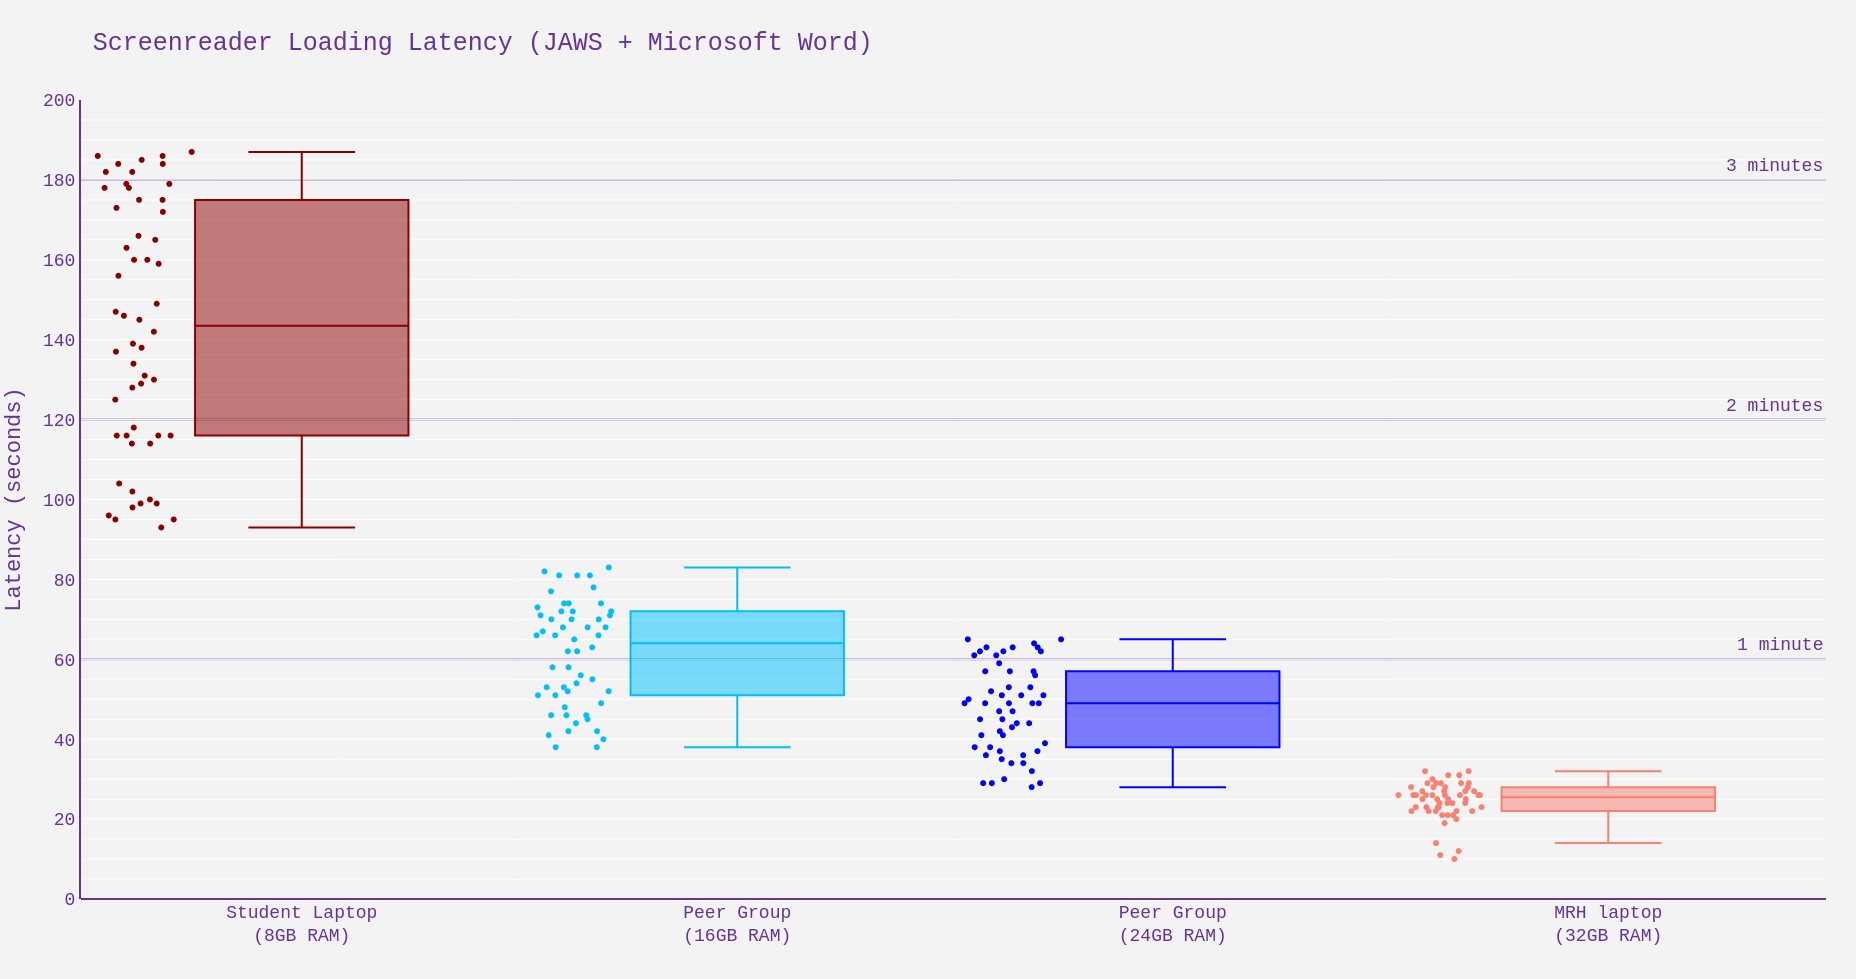
\includegraphics[width=\textwidth]{images/ComputerRBDisplaySpecsTVIFig1.png}

	\caption[Latency to Load JAWS]{Plot showing Latency to Load JAWS while Microsoft Word is open across a typical student laptop (Dell Latitude 3190 with 8GB RAM), a high quality student laptop (Dell Precision 3530 with 16GB RAM), a professional laptop (Lenovo ThinkPad E16 with 24GB RAM), and a high power laptop (Microsoft Surface Laptop 3 with 32GB RAM).}\label{fig:figure 1}
\end{figure}

\pagebreak
\hypertarget{screenreader-response}{}\section{Screenreader Responsiveness}\label{screenreader-response}
Measuring the latency of a screenreader to respond to key presses is important to determine if the laptop has sufficient RAM to run the software properly. If the laptop has insufficient RAM, the screenreader may take longer to respond to key presses, which can lead to delays in the user’s workflow. Measuring the latency of a screenreader can help identify if the laptop has enough RAM to run the software smoothly. This can help users avoid frustration and improve their productivity. Additionally, measuring the latency of a screenreader can help users identify if there are other issues with their laptop that may be causing the software to run slowly. By measuring the latency of a screenreader, users can ensure that their laptop is running optimally and that they are getting the most out of their software. Table \ref{tab:table5} provides these data for the same computers shown in Figure \ref{fig:figure 1}.

\pagebreak 
\large\textbf{Table \ref{tab:table5}}\normalfont 
\begin{longtable}[]{@{}
	>{\raggedright\arraybackslash}m{.5\textwidth}
	>{\raggedright\arraybackslash}m{.25\textwidth}
	>{\raggedright\arraybackslash}b{.25\textwidth}
	@{}
	}

	\toprule

	\textbf{Computer} \break (Color as Labelled in Figure 1)                                                                                                                                        & \textbf{Loading Time}\break (median [Range])                                                                                                               & \textbf{Response Lag}\break (median [Range])
	\\
	\midrule
	\endhead \hline                                                                                                                                                                                                                                                                                                                                                                                                                                                                                                                                                                                                                                                      \\
	\multicolumn{3}{r}{\textbf{Continued on Next Page}} \endfoot
	\endlastfoot
	\fcolorbox{red}{red}{\rule{0pt}{6pt}\rule{6pt}{0pt}}\qquad $\begin{array}{l}\textbf{Students Laptop}\footnote{\raggedright Dell Latitude 3190} \\ \text{8GB RAM}\end{array}$                                 & 143 [93-183] \footnote{\raggedright These are the data plotted in Figure 1 above. The responsiveness data are more clear when presented as a table here than as a plot} & 38 [27-91]\footnote{\raggedright It is further important to note here that any lag in screenreader responsiveness of \textgreater1 sec means the student is behind their peers and their educational opportunity is limited by the technology not being sufficient (\emph{i.e.}, not an adequate accommodation). } \\[1.0em]
	\fcolorbox{cyan}{cyan}{\rule{0pt}{6pt}\rule{6pt}{0pt}}\qquad $\begin{array}{l}\textbf{Student/Professional Laptop}\fnsep\footnote{\raggedright Dell Precision 3530} \\ \text{16GB RAM}\end{array}$           & 64 [38-93]                                                                                                                                                 & 9 [4-15]                                                                                                                                                                                                                                                                                              \\[1.0em]
	\fcolorbox{violet}{violet}{\rule{0pt}{6pt}\rule{6pt}{0pt}}\qquad$\begin{array}{l}\textbf{Professional Laptop}\footnote{\raggedright Lenovo ThinkPad E16 (TVI Personal Laptop)} \\ \text{24GB RAM}\end{array}$ & 49 [26-65]                                                                                                                                                 & 1 [0.05-2.5]                                                                                                                                                                                                                                                                                          \\[1.0em]
	\fcolorbox{orange}{orange}{\rule{0pt}{6pt}\rule{6pt}{0pt}}\qquad$\begin{array}{l}\textbf{Professional Laptop}\footnote{\raggedright Microsoft Surface 3 (My Personal Laptop)} \\ \text{32GB RAM}\end{array}$  & 25 [10-32]                                                                                                                                                 & 0.5 [0.01-1]\footnote{\raggedright 0.01 represents an immediate response that could not be measured}                                                                                                                                                                                                                     \\ [1.0em] \hline \caption{Lag in JAWS Reporting HTML Content}\label{tab:table5} \\
\end{longtable}

\pagebreak \hypertarget{notes-on-future-proofing-laptops}{}\section{Laptop Cost Factors}\label{notes-on-future-proofing-laptops}
Students with visual impairments require laptops that are compatible with assistive technology to receive a free and accessible public education. When selecting a laptop, there are several cost factors that must be taken into account. Firstly, the laptop should have sufficient RAM to run the assistive technology software smoothly. Secondly, the laptop should have a high-quality screen that is large enough to display text and images clearly. Thirdly, the laptop should have a long battery life to ensure that students can use it for extended periods of time without needing to recharge. Fourthly, the laptop should have a durable build quality to withstand daily wear and tear. Finally, the laptop should be lightweight and portable to enable students to carry it around easily. These factors can help ensure that students with visual impairments have access to the technology they need to succeed in their studies.

\hypertarget{future-proofing}{}\subsection{Laptop Durability}\label{future-proofing}

I asked ChatGPT why we should consider future usage needs of a laptop into my purchasing plans and here is its response (emphasis mine):

\begin{leftbar} \begin{quote}
		Buying laptops with high-end RAM and processor specifications can be beneficial for several reasons, especially in terms of longevity and performance. Here are some key considerations:

		\begin{enumerate}[leftmargin=*]
			\def\labelenumi{\arabic{enumi}.}

			\item
			      Future-Proofing:
		\end{enumerate}

		\begin{itemize}

			\item
			      Investing in higher-end components can help future-proof your laptop to some extent. As software and applications become more demanding over time, a laptop with better specifications is likely to remain relevant and capable of handling new software updates and requirements.
		\end{itemize}

		\begin{enumerate}[leftmargin=*]
			\def\labelenumi{\arabic{enumi}.}
			\setcounter{enumi}{1}

			\item
			      Multitasking and Performance:
		\end{enumerate}

		\begin{itemize}

			\item
			      Higher RAM allows for better multitasking capabilities. If you use resource-intensive applications or run multiple programs simultaneously, having ample RAM prevents slowdowns and ensures smooth performance.
			\item
			      A powerful processor can handle complex computations and tasks more efficiently, contributing to faster overall system performance.
		\end{itemize}

		\begin{enumerate}[leftmargin=*]
			\def\labelenumi{\arabic{enumi}.}
			\setcounter{enumi}{2}

			\item
			      Graphics Processing:
		\end{enumerate}

		\begin{itemize}

			\item
			      For tasks such as video editing, gaming, or other graphics-intensive applications, a high-end GPU (Graphics Processing Unit) is crucial. This is separate from RAM and the main processor but is equally important for certain tasks.
		\end{itemize}

		\begin{enumerate}[leftmargin=*]
			\def\labelenumi{\arabic{enumi}.}
			\setcounter{enumi}{3}

			\item
			      Long-Term Usability:
		\end{enumerate}

		\begin{itemize}

			\item
			      Technology advances quickly, and what is considered high-end today might become standard or entry-level in a few years. However, starting with a high-end laptop gives you a more extended period before your system becomes outdated.
		\end{itemize}

		\begin{enumerate}[leftmargin=*]
			\def\labelenumi{\arabic{enumi}.}
			\setcounter{enumi}{4}

			\item
			      Smooth Upgrades:
		\end{enumerate}

		\begin{itemize}

			\item
			      Some laptops allow users to upgrade certain components like RAM and storage. Starting with higher-end specifications provides more headroom for future upgrades, allowing you to extend the useful life of your laptop.
		\end{itemize}

		\begin{enumerate}[leftmargin=*]
			\def\labelenumi{\arabic{enumi}.}
			\setcounter{enumi}{5}

			\item
			      Resource-Intensive Applications:
		\end{enumerate}

		\begin{itemize}

			\item
			      If you use applications that require a lot of processing power, like video editing software, 3D modeling tools, or virtualization software, a high-end laptop can handle these tasks more efficiently, providing a better user experience.
		\end{itemize}

		\begin{enumerate}[leftmargin=*]
			\def\labelenumi{\arabic{enumi}.}
			\setcounter{enumi}{6}

			\item
			      Responsiveness and Speed:
		\end{enumerate}

		\begin{itemize}

			\item
			      A faster processor and more RAM contribute to a more responsive system. Applications load quicker, and the overall user experience is smoother, which can significantly impact productivity.
		\end{itemize}

		\begin{enumerate}[leftmargin=*]
			\def\labelenumi{\arabic{enumi}.}
			\setcounter{enumi}{7}

			\item
			      Enhanced Resale Value:
		\end{enumerate}

		\begin{itemize}

			\item
			      High-end laptops generally retain their value better than lower-end models. If you decide to sell or upgrade your laptop in the future, having top-tier specifications can make it more attractive to potential buyers.
		\end{itemize}

		It's important to note that the specific requirements depend on your usage patterns and needs. Not everyone needs the highest specifications, and sometimes a mid-range laptop can be more than sufficient for everyday tasks. However, \textbf{for users with demanding workloads or those who want a longer usable life from their device, opting for higher-end specifications can be a wise investment}.
	\end{quote}\end{leftbar}

\pagebreak	\hypertarget{optimizing-cost-with-performance}{}\subsection{Laptop Cost Optimization}\label{optimizing-cost-with-performance}

There is an economic theory based on a Terry Pratchett novel that explains this phenomenon better than we can. It is called the \href{http://en.wikipedia.org/wiki/Boots_theory}{Boots Theory}\footnote{\raggedright Full Text (emphasis mine):
	\begin{leftbar}
		\begin{quote}The reason that the rich were so rich, Vimes reasoned, was because they managed to spend less money.

			Take boots, for example. He earned thirty-eight dollars a month plus allowances. A really good pair of leather boots cost fifty dollars. But an affordable pair of boots, which were sort of OK for a season or two and then leaked like hell when the cardboard gave out, cost about ten dollars. Those were the kind of boots Vimes always bought, and wore until the soles were so thin that he could tell where he was in Ankh-Morpork on a foggy night by the feel of the cobbles.

			But the thing was that good boots lasted for years and years. \textbf{A man who could afford fifty dollars had a pair of boots that’d still be keeping his feet dry in ten years’ time, while the poor man who could only afford cheap boots would have spent a hundred dollars on boots in the same time and would still have wet feet.}

			Basically, \textbf{we are destined to be stuck in a cycle of perpetually spending more money for inferior products and will, in the end, spend more money than if we just paid for better product in the first place.} -- \textit{Men At Arms}, page 38
		\end{quote}
	\end{leftbar} 
 }

\hfill \break Table \ref{tab:table6} illustrates this theory in terms of student laptop computers (Assuming student has a laptop using a screenreader through 3rd-12th grade). Table \ref{tab:table6} also illustrates why we choose to err on the side of spending \$2000-3000 on a laptop computer that will last 3-5 years over spending \$1500-2000 on a laptop that will reach end-of-life within 1-2 years before becoming obsolete. By the end of 5 years we will have spent more on Low End and Mid Range Laptops than we would have otherwise spent had we purchased a High End Laptop. Importantly; however, we also would have been using laptops that always performed more poorly than a High End laptop would.

\pagebreak 
\large\textbf{Table \ref{tab:table6}}\normalfont 
\begin{longtable}[]{@{}
	>{\raggedright\arraybackslash}m{.15\textwidth}
	>{\raggedright\arraybackslash}m{.05\textwidth}
	>{\raggedright\arraybackslash}m{.05\textwidth}
	>{\raggedright\arraybackslash}m{.05\textwidth}
	>{\raggedright\arraybackslash}m{.05\textwidth}
	>{\raggedright\arraybackslash}m{.05\textwidth}
	>{\raggedright\arraybackslash}m{.05\textwidth}
	>{\raggedright\arraybackslash}m{.05\textwidth}
	>{\raggedright\arraybackslash}m{.05\textwidth}
	>{\raggedright\arraybackslash}m{.05\textwidth}
	>{\raggedright\arraybackslash}m{.05\textwidth}
	>{\raggedright\arraybackslash}b{.10\textwidth}@{}
	}
	\toprule                                                                                                                                                                                         &
	\multicolumn{10}{c}{\textbf{Does School Have to Purchase a Replacement Laptop by Year}}                                                                                                          &                                                                                                                                                                             \\[1.0em]
	\cline{2-11}                                                                                                                                                                                                                                                                                                                                                                   \\
	\textbf{RAM} \break Cost                                                                                                                                                                         & \textbf{1}   & \textbf{2}   & \textbf{3}   & \textbf{4}   & \textbf{5}   & \textbf{6}   & \textbf{7}   & \textbf{8}   & \textbf{9}   & \textbf{10}  & \textbf{10 year Cost} \\
	\midrule
	\endhead \hline                                                                                                                                                                                                                                                                                                                                                                \\
	\multicolumn{6}{r}{\textbf{Continued on Next Page}} \endfoot
	\endlastfoot
	\textbf{4GB}\footnote{\raggedright Dell Latitude 3190 Education}\fnsep\footnote{\raggedright The 4GB Laptop \textit{cannot} run JAWS and is included to show price comparison to the other options} \break \$525.04                 & $\checkmark$ & $\checkmark$ & $\checkmark$ & $\checkmark$ & $\checkmark$ & $\checkmark$ & $\checkmark$ & $\checkmark$ & $\checkmark$ & $\checkmark$ & \$5,250               \\[1.0em]
	\textbf{8GB}\footnote{\raggedright Dell Latitude 3190 Education}  \break \$1184                                                                                                                               & $\checkmark$ & $\checkmark$ & $\checkmark$ & $\checkmark$ & $\checkmark$ & $\checkmark$ & $\checkmark$ & $\checkmark$ & $\checkmark$ & $\checkmark$ & \$11,840              \\[1.0em]
	\textbf{16GB}\footnote{\raggedright Dell Precision 3530 given to TVIs teaching screenreaders} \break \$1751                                                                                                   & $\checkmark$ & -            & $\checkmark$ & -            & $\checkmark$ & -            & $\checkmark$ & -            & $\checkmark$ & -            & \$8,755               \\[1.0em]
\cdashline{1-12}\\
	\textbf{32GB}\footnote{\raggedright Microsoft Surface Laptop 3}\break \$2824\break \textcolor{red}{Best Case}\footnote{\raggedright This is my personal experience}                                                        & $\checkmark$ & -            & -            & -            & -            & $\checkmark$ & -            & -            & -            & -            & \$5,648               \\[1.0em] \\

	\textbf{32GB}\footnote{\raggedright Microsoft Surface Laptop 3}\break \$2824\break \textcolor{red}{Cautious}\footnote{\raggedright This is a conservative estimate to account for potential rough treatment of a computer} & $\checkmark$ & -            & -            & $\checkmark$ & -            & -            & $\checkmark$ & -            & -            & -            & \$8,472               \\[1.0em] \hline


	\caption[Cost of Laptops over Time]{Cost of Laptops Across Time. Notice that the final cost of the 32GB option is comparable to the 4GB over 10 years. However, the 4GB laptop is not capable of running JAWS reliably in the classroom setting.
	\break\textbullet For the \textcolor{red}{Best Case} Scenario, the 32GB laptop is between \$3,107 and \$6,192 \textit{\textbf{cheaper}} over time compared to the 16GB and 8GB laptops, respectively.
	\break\textbullet For the \textcolor{red}{Cautious} Scenario, the 32GB laptop is between \$283 and \$3,386 \textit{\textbf{cheaper}} over time compared to the 16GB and 8GB laptops, respectively}\label{tab:table6}
\end{longtable}

\pagebreak
\hypertarget{minimum-laptop-recommendations}{}\section{Recommended Laptop Specifications}\label{minimum-laptop-recommendations}
Table \ref{tab:table7} is a list of recommendations for laptop specifications by use case.

\pagebreak 
\large\textbf{Table \ref{tab:table7}}\normalfont 
\begin{longtable}[]{@{}
	>{\raggedright\arraybackslash}m{.7\textwidth}
	>{\raggedright\arraybackslash}b{.3\textwidth}@{}
	}
	\toprule

	\textbf{Use Case}                                                                                                                                                                                                                                                                & \textbf{Recommendation}      \\
	\midrule
	\endhead \hline                                                                                                                                                                                                                                                                                                 \\
	\multicolumn{2}{r}{\textbf{Continued on Next Page}} \endfoot
	\endlastfoot
	\multicolumn{2}{l}{\textbf{Screenreader Only}}                                                                                                                                                                                                                                                \\[1em]
	JAWS Screenreader\footnote{\raggedright Although NVDA, ZDSR, and Dolphin Screenreader have been widely available for \textgreater10 years, JAWS is considered the industry standard and is the one primarily supported by Industry in the United States as well as Vocational Rehabilitation} & \textgreater\textbf{24-32GB} \\[1.0em]
	NVDA Screenreader                                                                                                                                                                                                                                                                & \textgreater\textbf{24-32GB} \\[1.0em]
	Dolphin Screenreader                                                                                                                                                                                                                                                             & \textgreater\textbf{24-32GB} \\[1.0em]
	ZDSR Screenreader                                                                                                                                                                                                                                                                & \textgreater\textbf{24-32GB} \\[1.0em]
	\multicolumn{2}{l}{\textbf{ Screen Magnification Only}}                                                                                                                                                                                                                                       \\[1em]
	ZoomText                                                                                                                                                                                                                                                                         & \textgreater\textbf{24-32GB} \\[1.0em]
	Windows Magnifier                                                                                                                                                                                                                                                                & \textgreater\textbf{16GB}    \\[1.0em]
	Dolphin SuperNova                                                                                                                                                                                                                                                                & \textgreater\textbf{24-32GB} \\[1.0em]
	\multicolumn{2}{l}{\textbf{Screenreader + Magnification}}                                                                                                                                                                                                                                     \\[1em]
	JAWS Screenreader + Windows Magnifier                                                                                                                                                                                                                                            & \textgreater\textbf{24-32GB} \\[1.0em]
	NVDA Screenreader + Windows Magnifier                                                                                                                                                                                                                                            & \textgreater\textbf{24-32GB} \\[1.0em]
	ZDSR Screenreader + Windows Magnifier                                                                                                                                                                                                                                            & \textgreater\textbf{24-32GB} \\[1.0em]
	Dolphin Screenreader + Windows Magnifier                                                                                                                                                                                                                                         & \textgreater\textbf{24-32GB} \\[1.0em]
	SuperNova Screenreader + Magnification                                                                                                                                                                                                                                           & \textgreater\textbf{32-64GB} \\[1.0em]
	Fusion Screenreader + Magnification                                                                                                                                                                                                                                              & \textgreater\textbf{32-64GB} \\[1.0em] \hline
	\caption{Recommended Laptop Specifications}\label{tab:table7}
\end{longtable}

\pagebreak
\hypertarget{laptops-meeting-recommended-specifications}{}\section{Laptops Meeting Specifications}\label{laptops-meeting-recommended-specifications}
Table \ref{tab:table8} is an alphabetical list of laptop computers that meet the recommended specifications defined in Table \ref{tab:table7}.

\pagebreak 
\large\textbf{Table \ref{tab:table8}}\normalfont 
\begin{longtable}[]{@{}
	>{\raggedright\arraybackslash}m{.3\textwidth}
	>{\raggedright\arraybackslash}m{.12\textwidth}
	>{\raggedright\arraybackslash}m{.12\textwidth}
	>{\raggedright\arraybackslash}m{.12\textwidth}
	>{\raggedright\arraybackslash}m{.12\textwidth}
	>{\raggedright\arraybackslash}b{.2\textwidth}@{}
	}
	\toprule

	\textbf{Company / Model}                                                                                    & \textbf{Cost}                                                                                                                                   & \textbf{Keyboard}      & \textbf{RAM} & \textbf{Screen Size} & \textbf{Processor} \\
	\midrule
	\endhead \hline                                                                                                                                                                                                                                                                                                                                   \\
	\multicolumn{6}{r}{\textbf{Continued on Next Page}} \endfoot
	\endlastfoot
	Acer Predator Helios 16                                                                                     & \$2,499                                                                                                                                         & QWERTY                 & 32GB         & 16.0''               & 13th Gen i9        \\[1.0em]
	Acer Predator Triton                                                                                        & \$3,799                                                                                                                                         & QWERTY                 & 64GB         & 17.0''               & 13th Gen i9        \\[1.0em]
	Alienware m16                                                                                               & \$3,499                                                                                                                                         & QWERTY                 & 32GB         & 16.0''               & 13th Gen 19        \\[1.0em]
	Alienware x14                                                                                               & \$1,999                                                                                                                                         & QWERTY                 & 32GB         & 14.0''               & 13th Gen i7        \\[1.0em]
	Asus ProArt Studiobook                                                                                      & \$2,999                                                                                                                                         & QWERTY                 & 32GB         & 16.0''               & 13th Gen i9        \\[1.0em]
	Asus Zenbook Pro 16X                                                                                        & \$2,599                                                                                                                                         & QWERTY                 & 32GB         & 16.0''               & 13th Gen i9        \\[1.0em]
	b.book\footnote{\raggedright This is a Windows Computer without a monitor, substituting a 40 cell braille display}                                                                                        & \$5,765                                                                                                                                        & Perkins                 & 8GB-16GB\footnote{\raggedright This is included despite low RAM values since it is a custom modified product} & none               & 13th Gen i9        \\[1.0em]
 Dell G16 Gaming Laptop                                                                                      & \$1,999                                                                                                                                         & QWERTY                 & 32GB         & 16.0''               & 13th Gen i7        \\[1.0em]
	Dell Inspiron 16 Plus                                                                                       & \$1,499                                                                                                                                         & QWERTY                 & 32GB         & 16.0''               & 13th Gen i7        \\[1.0em]
	Dell Precision 3480                                                                                         & \$3,205                                                                                                                                         & QWERTY                 & 32GB         & 14.0''               & 13th Gen i7        \\[1.0em]
	Dell Precision 3581                                                                                         & \$3,854                                                                                                                                         & QWERTY                 & 32GB         & 15.6''               & 13th Gen i7        \\[1.0em]
	Dell Precision 5480                                                                                         & \$4,354                                                                                                                                         & QWERTY                 & 32GB         & 14.0''               & 13th Gen i7        \\[1.0em]
	Dell Precision 5770                                                                                         & \$2,789                                                                                                                                         & QWERTY                 & 32GB         & 17''                 & 12th Gen i7        \\[1.0em]
	Dell XPS 13 Plus                                                                                            & \$2,009                                                                                                                                         & QWERTY                 & 32GB         & 13.4''               & 13th Gen i7        \\[1.0em]
	Dell XPS 15                                                                                                 & \$2,349                                                                                                                                         & QWERTY                 & 32GB         & 15.6''               & 12th Gen i9        \\[1.0em]
	Dell XPS 15                                                                                                 & \$2,999                                                                                                                                         & QWERTY                 & 32GB         & 15.6''               & 13th Gen i9        \\[1.0em]
	Dell XPS 17                                                                                                 & \$3,349                                                                                                                                         & QWERTY                 & 32GB         & 15.6''               & 13th Gen i7        \\[1.0em]
	Dell XPS 17                                                                                                 & \$3,549                                                                                                                                         & QWERTY                 & 32GB         & 15.6''               & 13th Gen i9        \\[1.0em]
	Dell Latitude 7440                                                                                          & \$3,615                                                                                                                                         & QWERTY                 & 32GB         & 14.0''               & 13th Gen i7        \\[1.0em]
	Dell Precision 5680                                                                                         & \$5,597                                                                                                                                         & QWERTY                 & 32GB         & 16.0''               & 13th Gen i9        \\[1.0em]
	Dell Precision 7680                                                                                         & \$7,225                                                                                                                                         & QWERTY                 & 32GB         & 16.0''               & 13th Gen i9        \\[1.0em]
	Framework 13                                                                                                & \$1,102                                                                                                                                         & QWERTY                 & 32GB         & 13.5''               & 13th Gen i7        \\[1.0em]
	Framework 13                                                                                                & \$1,732                                                                                                                                         & QWERTY                 & 32GB         & 13.5''               & AMD Ryzen 7        \\[1.0em]
	Framework 13                                                                                                & \$1,892                                                                                                                                         & QWERTY                 & 64GB         & 13.5''               & AMD Ryzen 7        \\[1.0em]
	Framework 13                                                                                                & \$2,222                                                                                                                                         & QWERTY                 & 64GB         & 13.5''               & 13th Gen i7        \\[1.0em]
	Framework 16                                                                                                & \$2,239                                                                                                                                         & QWERTY & 32GB         & 16.0''               & AMD Ryzen 9        \\[1.0em]
	Framework 16                                                                                                & \$2,399                                                                                                                                         & QWERTY & 64GB         & 16.0''               & AMD Ryzen 9        \\[1.0em]
	Framework 16\footnote{\raggedright includes a built in AMD Graphics Processing Unit (GPU)}                                                                              & \$2,639                                                                                                                                         & QWERTY & 32GB         & 16.0''               & AMD Ryzen 9        \\[1.0em]
	Framework 16\footnote{\raggedright includes a built in AMD Graphics Processing Unit (GPU)}                                                                              & \$2,799                                                                                                                                         & QWERTY & 64GB         & 16.0''               & AMD Ryzen 9        \\[1.0em]
	HP Dragonfly Pro                                                                                            & \$1,549                                                                                                                                         & QWERTY                 & 32GB         & 14.0''               & AMD Ryzen 7        \\[1.0em]
	HP Envy                                                                                                     & \$1,749                                                                                                                                         & QWERTY                 & 32GB         & 17.3''               & 13th Gen i7        \\[1.0em]
	Legion Pro 7i                                                                                               & \$3,599                                                                                                                                         & QWERTY                 & 32GB         & 16.0''               & 13th Gen i9        \\[1.0em]
	Lenovo ThinkPad P16 Gen 2                                                                                   & \$2,039                                                                                                                                         & QWERTY                 & 32GB         & 16.0''               & AMD Ryzen 7        \\[1.0em]
	Lenovo ThinkPad P16 Gen 2                                                                                   & \$2,829                                                                                                                                         & QWERTY                 & 64GB         & 16.0''               & AMD Ryzen 7        \\[1.0em]
	Lenovo ThinkPad P16 Gen 2                                                                                   & \$3,239                                                                                                                                         & QWERTY                 & 32GB         & 16.0''               & 13th Gen i7        \\[1.0em]
	Lenovo ThinkPad P16 Gen 2                                                                                   & \$4,189                                                                                                                                         & QWERTY                 & 64GB         & 16.0''               & 13th Gen i7        \\[1.0em]
	Lenovo ThinkPad P16v                                                                                        & \$3,339                                                                                                                                         & QWERTY                 & 32GB         & 16.0''               & 13th Gen i7        \\[1.0em]
	Lenovo ThinkPad P16v                                                                                        & \$4,929                                                                                                                                         & QWERTY                 & 64GB         & 16.0''               & 13th Gen i7        \\[1.0em]
	Lenovo Thinkpad P14s                                                                                        & \$2,199                                                                                                                                         & QWERTY                 & 32GB         & 14.0''               & AND Ryzen 7        \\[1.0em]
	Lenovo Thinkpad P14s                                                                                        & \$2,509                                                                                                                                         & QWERTY                 & 64GB         & 14.0''               & AND Ryzen 7        \\[1.0em]
	Lenovo Thinkpad X1 Yoga                                                                                     & \$3,719                                                                                                                                         & QWERTY                 & 32GB         & 14.0''               & 13th Gen i7        \\[1.0em]
MSI Alpha 17  & \$1,849  & QWERTY  & 32GB & 17.3''  & AMD Ryzen9 \\[1.0em]
MSI Bravo 17 & \$1,499  & QWERTY  & 32GB & 17.3''  & AMD Ryzen7 \\[1.0em]
MSI Katana 15 & \$1,899  & QWERTY  & 32GB & 15.6''  & 13th Gen i9 \\[1.0em]
MSI Pulse 15 & \$1,699  & QWERTY  & 32GB & 15.6''  & 13th Gen i7 \\[1.0em]
MSI Pulse 17 & \$1,899  & QWERTY  & 32GB & 17.3''  & 13th Gen i9 \\[1.0em]
MSI Raider 15 & \$1,999  & QWERTY  & 32GB & 15.6''  & 13th Gen i9 \\[1.0em]
MSI Vector & \$1,999  & QWERTY  & 32GB & 17.3''  & 13th Gen i9 \\[1.0em]
	Microsoft Surface Laptop 5                                                                                  & \$2824                                                                                                                                          & QWERTY                 & 32GB         & 15.0''               & 12th Gen i7        \\[1.0em]
	Orbit Optima\footnote{\raggedright This is a Windows Computer without a monitor, substituting a 40 cell braille display} & \$6,500                                                                                                                                         & QWERTY                 & 32GB-64GB    & none                 & 13th Gen i7        \\ [1.0em]
		Razer Blade 15 & \$2,999 & QWERTY & 32GB & 15.6'' & 13th Gen i7  \\[1.0em]
Seika Studio\footnote{\raggedright This is a Windows Computer without a monitor, substituting a 40 cell braille display} & \$6,500                                                                                                                                         & QWERTY                 & 8GB-16GB\footnote{\raggedright This is included despite low RAM values since it is a custom modified product}     & none                 & 12th Gen i7        \\ [1.0em]\hline
	\caption[{Laptop Computers Meeting Specifications}]{Laptop Computers Meeting Recommended Specifications}\label{tab:table8}
\end{longtable}
\cleardoublepage\chapter{Transformative Tablets: Pioneering Success for Visually Impaired Students Through Innovative Apps}\label{ios-devices}

In an era where technology shapes the landscape of education, tablets have emerged as transformative tools, providing visually impaired students with unprecedented access to knowledge and fostering independence in their academic journeys.\footnote{I am omitting iPhone and Android phones from this document as the purchase of student phones is beyond the purview of a school district. However, iOS apps are provided as many of these are available on both Tablets and Phones and training students to use the technology on their personal device is often necessary, particularly within the auspice of Orientation \& Mobility instruction} Both iPad and Android devices offer user-friendly interfaces and a diverse array of applications specifically tailored to bridge the accessibility gap. This chapter explores how tablets, in tandem with purpose-built apps, are not just tools but catalysts for success in the educational journey of visually impaired students.

Tablets serve as dynamic portals for visually impaired learners, offering a multi-sensory approach to engagement. Their unique functionalities, combined with a robust ecosystem of accessibility apps, empower students to navigate the digital realm with confidence and independence.

\section{Tablet Considerations}\label{tablet-considerations}

When selecting a tablet for students with visual impairments, consider the following:

\begin{itemize}
    \item \emph{Accessibility features:} Ensure compatibility with screen readers and magnification tools (e.g., VoiceOver for iOS, TalkBack for Android).\footnote{Traditionally, assistive technology for the blind has focused on the iPad line since the Android line had historically lagged behind the Apple products for accessibility features prior to 2020 so accessibility apps have favored the iOS/iPadOS architecture. However, groups are emerging that specifically instruct users of Android devices how to access and use accessibility settings \emph{cf.}, \href{http://www.youtube.com/channel/UCvEM-SmpwElNALldhp8hG1g}{Blind Android Users}}
    \item \emph{Tactile features, size, and weight:} Choose a device that accommodates the student's specific needs.
    \item \emph{Contrast and color settings:} High contrast and customizable color settings, as well as text-to-speech functionalities, enhance readability.
    \item \emph{Screen size:} Larger screens can help reduce visual fatigue and improve usability, but balance with portability.
    \item \emph{App compatibility:} Ensure the device supports a variety of educational and accessibility apps.
    \item \emph{Visual fatigue:} Avoid prioritizing brightness; instead, focus on resolution and screen area. Adjust luminance for students with photophobia.
\end{itemize}

Contrast ratio is especially important for students with visual impairments. Understanding and prioritizing contrast ratio helps foster an inclusive and enriching educational environment.

\section{Tablet Options}\label{tab:tablet-options}
When choosing an Android Tablet or iPad for a student with visual impairments, several factors must be considered to ensure that the student receives free and appropriate public education. The first factor to consider is the screen contrast ratio. A high contrast ratio is essential for students with visual impairments as it makes it easier for them to read text and view images on the screen. For Android Tablets, the W3C recommends a contrast ratio of at least 4.5:1 for small text and 3.0:1 for large text\footnote{\raggedright \href{https://support.google.com/accessibility/android/answer/7158390?hl=en}{Google. (n.d.). Color contrast - Android Accessibility Help. Retrieved December 19, 2023}}. On the other hand, Apple devices have an “Increase Contrast” feature that can be turned on to make text and other elements more visible\footnote{\raggedright \href{https://www.imore.com/how-increase-contrast-visual-accessibility-iphone-and-ipad}{iMore. (n.d.). How to increase contrast for visual accessibility on iPhone and iPad. Retrieved December 19, 2023}}.

The second factor to consider is the size of the screen. A larger screen is beneficial for students with visual impairments as it allows them to view text and images more clearly. Tablets usually have larger screens than smartphones, making them a better choice for students with visual impairments\footnote{\raggedright \href{https://www.afb.org/blindness-and-low-vision/using-technology/cell-phones-tablets-mobile/smartphone-or-tablet-which}{American Foundation for the Blind. (n.d.). Smartphone or Tablet: Which is Best for You? Retrieved December 19, 2023}}. However, it is important to note that larger screens come at the expense of portability. Therefore, it is essential to find a balance between screen size and portability.

The third factor to consider is the availability of accessible apps. Both Android and iOS devices have built-in accessibility features such as screen readers, magnifiers, and high contrast modes \footnote{\raggedright \href{https://www.aao.org/eye-health/tips-prevention/low-vision-impairment-apps-tech-assistive-devices }{American Academy of Ophthalmology. (n.d.). 30 Apps, Devices and Technologies for People With Vision Impairments. Retrieved December 19, 2023}}\footnote{\raggedright \href{https://www.afb.org/blindness-and-low-vision/using-technology/cell-phones-tablets-mobile/apple-ios-iphone-and-ipad }{American Foundation for the Blind. (n.d.). Apple iOS for iPhone and iPad: Considerations for Users with Visual Impairments. Retrieved December 19, 2023}}. Additionally, there are several apps available that are specifically designed for students with visual impairments. For example, the “Lookout” app for Android provides spoken feedback about things around you, while the “Be My Eyes” app connects visually-impaired people with sighted volunteers through a live video call\footnote{\raggedright \href{https://www.aao.org/eye-health/tips-prevention/technology-apps-devices-children-blind-low-vision}{American Academy of Ophthalmology. (n.d.). Technology Tools for Children with Low Vision. Retrieved December 19, 2023}}. It is important to ensure that the device has access to these apps to ensure that the student can receive free and appropriate public education.
\emph{Table \ref{tab:modern-laptop-specs}} describes current tablet computers that are available for students with visual impairments.

\subsection{AndroidOS 13+ Tablets}
\tagpdfsetup{table/header-rows={1}}
\begin{longtblr}[
  caption = {AndroidOS 13+ tablets suitable for students with visual impairments},
  label = {tab:android-tablets},
  remark{Note} = {Summary: Comprehensive list of Android tablets running OS 13 or higher, showing model name and screen size in inches}
]{
  colspec = {X[l] X[l]},
  rowhead = 1,
  hlines,
  stretch = 1.5
}
Tablet & Screen Size \\
Acer Iconia Tab P10 & 10.4 \\
Alldocube iPlay 50 mini Pro NFE & 8.4 \\
Alldocube iPlay 60 & 10.9 \\
Blackview OSCAL Pad 16 & 10.5 \\
Doogee U10 Pro & 10.1 \\
Galaxy Tab A9 & 8.7 \\
Galaxy Tab A9+ & 11.0 \\
Google Pixel Tablet & 10.9 \\
Honor Tablet Pad 9 & 12.1 \\
Hyundai HyTab 7 & 7.0 \\
Lenovo Tab Extreme & 14.5 \\
Lenovo Tab M10 5G & 10.6 \\
Lenovo Tab M10 Plus (3rd Gen) & 10.6 \\
Lenovo Tab M7 (3rd gen.) & 7.0 \\
Lenovo Tab M8 (4th Gen) & 8.0 \\
Lenovo Tab M9 & 9.0 \\
Lenovo Tab P11 (2nd gen) & 11.5 \\
Lenovo Tab P11 Plus & 11.0 \\
Lenovo Tab P11 Pro (2nd Gen) & 11.2 \\
Lenovo Tab P12 & 12.7 \\
Lenovo Tab P12 Pro & 12.6 \\
Lenovo Xiaoxin Pad 2024 & 11.0 \\
Lenovo Yoga Tab 11 & 11.0 \\
Lenovo Yoga Tab 13 & 13.0 \\
Nokia T10 & 8.0 \\
Nokia T20 & 10.4 \\
Nokia T21 & 10.4 \\
OnePlus Pad & 11.6 \\
Oppo Pad Air 2 & 11.4 \\
Oscal Pad 18 & 11.0 \\
Razer Edge & 6.8 \\
Redmi Pad & 10.61 \\
Redmi Pad SE & 11.0 \\
Samsung Galaxy Tab A7 Lite & 8.7 \\
Samsung Galaxy Tab A8 & 10.5 \\
Samsung Galaxy Tab Active3 & 8.0 \\
Samsung Galaxy Tab S7 FE & 12.4 \\
Samsung Galaxy Tab S9 & 11.0 \\
Samsung Galaxy Tab S9 FE & 10.9 \\
Samsung Galaxy Tab S9 FE+ & 12.4 \\
Samsung Galaxy Tab S9 Ultra & 14.6 \\
Samsung Galaxy Tab S9+ & 12.4 \\
Teclast P30T & 10.1 \\
Teclast T60 & 12.0 \\
UMIDIGI A15 Tab & 11.0 \\
Vivo Pad 2 & 12.1 \\
Xiaomi Pad 6 & 11.0 \\
Xiaomi Pad 6 Pro & 11.0 \\
ZTE Nubia Pad 3D & 12.4 \\
\end{longtblr}

\subsection{iPadOS Tablets}
\tagpdfsetup{table/header-rows={1}}
\begin{longtblr}[
  caption = {iPadOS tablets suitable for students with visual impairments},
  label = {tab:ios-tablets},
  note = {Current Apple iPad models with their costs and screen sizes, arranged by model type}
]{
  colspec = {X[l] X[l] X[l]},
  rowhead = 1,
  row{1} = {font=\bfseries},
  hlines,
  stretch = 1.5
}
Tablet & Cost & Screen Size \\
Apple iPad 10.2 & \$269 & 10.2 \\
Apple iPad 10.9 & \$449 & 10.9 \\
Apple iPad Air 5 & \$599 & 10.9 \\
Apple iPad Pro 11 & \$799 & 11.0 \\
Apple iPad Pro 12.9 & \$1099 & 12.9 \\
Apple iPad mini 6 & \$499 & 8.3 \\
\end{longtblr}

\subsection{Windows OS Tablets}
\tagpdfsetup{table/header-rows={1}}
\centering
\begin{longtblr}[
  caption = {Windows OS tablets suitable for students with visual impairments},
  label = {tab:windows-tablets},
  note = {Windows-based tablets and 2-in-1 devices suitable for visually impaired students, listing model, price, and display size}
]{
  colspec = {X[l] X[l] X[l]},
  rowhead = 1,
  row{1} = {font=\bfseries},
  hlines,
  stretch = 1.5
}
Tablet & Cost & Screen Size \\
 Alldocube & \$669 & 12.6 \\
 Asus ROG Flow Z13 & \$1799 & 13.4 \\
Asus ROG Flow Z13 (2023) & \$1799 & 13.4 \\
Asus Vivobook 13 Slate OLED & \$749 & 13.3 \\
Dell XPS 13 & \$1099 & 13.0 \\
Huawei MateBook E & \$1419 & 12.6 \\
Lenovo Yoga Duet & \$970 & 13.0 \\
Microsoft Surface Book 3 13.5 & \$799 & 13.5 \\
Microsoft Surface Book 3 15 & \$1159 & 15.0 \\
Microsoft Surface Go 3 & \$399 & 10.5 \\
Microsoft Surface Go 3 & \$629 & 10.5 \\
Microsoft Surface Go 4 & \$579 & 10.5 \\
Microsoft Surface Pro 9 & \$979 & 13.0 \\
\end{longtblr}

\subsection{ChromeOS Tablets}
\tagpdfsetup{table/header-rows={1}}
\begin{longtblr}[
  caption = {ChromeOS tablets suitable for students with visual impairments},
  label = {tab:chromeOS-tablets},
  note = {Available ChromeOS tablets and their specifications, focusing on cost-effective options for educational use}
]{
  colspec = {X[l] X[l] X[l]},
  rowhead = 1,
  row{1} = {font=\bfseries},
  hlines,
  stretch = 1.5
}
Tablet & Cost & Screen Size \\
Acer Chromebook Tab 10 & \$299 & 9.7 \\
Asus Chromebook CM3 & \$369 & 10.5 \\
Asus Chromebook Tablet CT100 & \$299 & 9.7 \\
Fydetab Duo & \$630 & 12.4 \\
Google Pixel Slate & \$499 & 12.3 \\
HP Chromebook x2 11 & \$599 & 11.0 \\
Lenovo Chromebook Duet 3 & \$349 & 11.0 \\
Lenovo Chromebook Duet 5 & \$379 & 13.3 \\
\end{longtblr}

\section{Mobile Applications}\label{tab:tablelet-apps}
Mobile apps run on tablets are becoming increasingly important for students with visual impairments to access a free and appropriate public education. These apps can provide students with access to digital content, assistive technology, and other tools that can help them succeed in their studies. High-quality mobile apps can help students with visual impairments access the same educational materials as their sighted peers and participate fully in the curriculum. They can also help improve literacy skills, comprehension, and productivity. In this section, we will explore the importance of high-quality mobile apps for students with visual impairments and discuss some of the best apps available on the market today. \emph{Table \ref{tab:table10}} gives a list of current apps available for use with students with visual impairments.

\subsection{Accessibility Training/Auditory Games}
\begin{longtblr}[
  caption = {Mobile apps for accessibility training and auditory games for students with visual impairments},
  label = {tab:chapter2:accessibility-training-apps},
  note = {Educational apps designed to teach screen reader gestures and provide auditory game experiences, including pricing and platform availability}
]{
  colspec = {X[l] X[l] X[l] X[l]},
  rowhead = 1,
  row{1} = {font=\normalfont},
  hlines,
  stretch = 1.5,
}
App & Cost & Function & OS \\
CosmoBally in Space & free & Train VoiceOver Gestures & iOS/iPadOS \\
Ballyland Magic Plus & \$3.99 & Train VoiceOver Gestures & iOS/iPadOS \\
Ballyland Rotor & \$2.99 & Train VoiceOver rotor & iOS/iPadOS \\
Ballyland Stay Still Squeaky! & \$2.99 & Train VoiceOver Gestures & iOS/iPadOS \\
Blindfold Games Launcher & free\footnote{\raggedright Games purchased separately} & Sonic Games & iOS/iPadOS \\
Blindfold Tap and Swipe & free & Train VoiceOver Gestures & iOS/iPadOS \\
ObjectiveEd Games & free\footnotemark[\value{footnote}] & Sonic Games & iOS/iPadOS \\
VO Lab & \$4.99 & Train VoiceOver Gestures & iOS/iPadOS \\
Screenreader & free & Train Accessibility Gestures & iOS/iPadOS, Android 13+ \\
\end{longtblr}

\subsection{Cortical Vision Impairment}
\begin{longtblr}[
  caption = {Mobile apps for cortical vision impairment (CVI) training for students with visual impairments},
  remark{Note} = {Summary: Specialized apps designed for CVI training and assessment, including pricing and supported platforms},
  label = {tab:chapter2:cvi-training-apps}
]{
  colspec = {X[l] X[l] X[l] X[l]},
  rowhead = 1,
  row{1} = {font=\normalfont},
  hlines,
  stretch = 1.5,
}
App & Cost & Function & OS \\
Art of Glow & free & CVI-based Vision Training & iOS/iPadOS \\
Big Band Patterns & \$34.99 & CVI-based Vision Training & iOS/iPadOS \\
Big Bang Pictures & \$34.99 & CVI-based Vision Training & iOS/iPadOS \\
CVI Connect & \$10/mo & CVI-based Vision Training & iOS/iPadOS \\
CVI Connect Pro & free\footnote{\raggedright Annual Price Per Enrolled Student: 1-5=\$300\quad6-10=\$250\quad11-15=\$200\quad16-19=\$150} & CVI-based Vision Training & iOS/iPadOS \\
CVI Toddler Visual Eye Train & free & CVI-based Vision Training & iOS/iPadOS \\
CVI Training (Color) & free & CVI-based Vision Training & iOS/iPadOS \\
CVI Training (Human face) & free & CVI-based Vision Training & iOS/iPadOS \\
CVI Training (Pattern) & free & CVI-based Vision Training & iOS/iPadOS \\
CVI Training (Recognition) & free & CVI-based Vision Training & iOS/iPadOS \\
CVI Training (Visual Tracking) & free & CVI-based Vision Training & iOS/iPadOS \\
Dexteria VMI & \$5.99 & CVI-based Vision Training & iOS/iPadOS \\
Doodle Kids & free & CVI-based Vision Training & iOS/iPadOS \\
EDA Play & \$4.99 & CVI-based Vision Training & iOS/iPadOS \\
EDA Play ELIS & \$2.99 & CVI-based Vision Training & iOS/iPadOS \\
EDA Play PAULI & \$2.99 & CVI-based Vision Training & iOS/iPadOS \\
EDA Play TOBY & free & CVI-based Vision Training & iOS/iPadOS \\
EDA Play TOM & free & CVI-based Vision Training & iOS/iPadOS \\
EyeMove & free & CVI-based Vision Training & iOS/iPadOS \\
Fludity HD & free & CVI-based Vision Training & iOS/iPadOS \\
Little Bear Sees & \$4.99 & CVI-based Vision Training & iOS/iPadOS \\
P.O.V. Spatial Reasoning & \$3.99 & CVI-based Vision Training & iOS/iPadOS \\
Peekaboo Barn & \$2.99 & CVI-based Vision Training & iOS/iPadOS \\
Sensory Electra & free & CVI-based Vision Training & iOS/iPadOS \\
Sensory Light Box & \$3.99 & CVI-based Vision Training & iOS/iPadOS \\
Tap-n-See Now & \$2.99 & CVI-based Vision Training & iOS/iPadOS \\
VO Lab & free & CVI-based Vision Training & iOS/iPadOS \\
Visual Attention Therapy Lite & free & CVI-based Vision Training & iOS/iPadOS \\
\end{longtblr}

\subsection{Audiobook/Reading}
\begin{longtblr}[
  caption = {Mobile apps for audiobook, e-book, and DAISY reading for students with visual impairments},
  label = {tab:chapter2:audiobook-reading-apps}
]{
  colspec = {X[l] X[l] X[l] X[l]},
  rowhead = 1,
  row{1} = {font=\normalfont},
  hlines,
  stretch = 1.5,
}
App & Cost & Function & OS \\
Audible & free\footnote{\raggedright requires books to be purchased} & Audiobook & iOS/iPadOS, AndroidOS 13+ \\
BARD Mobile & free\footnote{\raggedright requires account with local affiliate State Library for the Blind} & e-Book & iOS/iPadOS, AndroidOS 13+ \\
Bookshare Reader & free & DAISY Reader & iOS/iPadOS \\
Dolphin EasyReader & free & DAISY Reader & iOS/iPadOS, AndroidOS 13+ \\
KNFB Reader (OneStepReader) & \$99.99 & OCR/Reading & iOS/iPadOS, AndroidOS 13+ \\
Kindle & free\footnotemark[12] & e-Book & iOS/iPadOS, AndroidOS 13+ \\
Libby & free\footnotemark[13] & Audiobook & iOS/iPadOS, AndroidOS 13+ \\
VoiceDream Reader & free\footnote{\raggedright requires \$79.99/yr subscription and additional \$4.99 for each premium voice} & DAISY Reader & iOS/iPadOS \\
\end{longtblr}

\subsection{Productivity/Schoolwork/Optical Character Recognition}
\begin{longtblr}[
  caption = {Mobile apps for audiobook, e-book, and DAISY reading for students with visual impairments},
  label = {tab:chapter2:audiobook-reading-apps}
]{
  colspec = {X[l] X[l] X[l] X[l]},
  rowhead = 1,
  row{1} = {font=\normalfont},
  hlines,
  stretch = 1.5,
}
App & Cost & Function & OS \\
Aiko & free & AI Speech to text & iOS/iPadOS \\
Ballyland Code 1: Say Hello & \$2.99 & Auditory Coding & iOS/iPadOS \\
Ballyland Code 2: Give Rotor & \$2.99 & Auditory Codings & iOS/iPadOS \\
Ballyland Code 3: Pick Up & \$2.99 & Auditory Coding & iOS/iPadOS \\
Clusiv & free\footnote{\raggedright Full access provided through Vocational Rehabilitation} & Online learning platform\footnote{\raggedright Clusiv is an online learning platform for the blind and visually impaired that teaches occupational training, technology skills, and educational courses to empower employment} & iOS/iPadOS \\
Clusive & free & Online learning platform\footnote{\raggedright Clusive is an open-source online learning platform for the blind and visually impaired} & iOS/iPadOS \\
Code Quest & free & Auditory Coding & iOS/iPadOS \\
Desmos Graphing Calculator & free & Accessible Graphing & iOS/iPadOS, AndroidOS 13+ \\
Desmos Scientific Calculator & free & Accessible Scientific Calculator & iOS/iPadOS, AndroidOS 13+ \\
Envision AI & free & OCR & iOS/iPadOS, AndroidOS 13+ \\
GoodNotes & free\footnote{\raggedright with in app purchases} & Scan \& Markup Documents & iOS/iPadOS, AndroidOS 13+ \\
KNFB Reader (OneStepReader) & \$99.99 & OCR/Reading & iOS/iPadOS, AndroidOS 13+ \\
My Board Buddy & free & local view of class blackboard & iOS/iPadOS \\
Notability & free\footnote{\raggedright with in app purchases} & Scan \& Markup Documents & iOS/iPadOS, AndroidOS 13+ \\
QuickScanner & free\footnote{\raggedright a paid subscription removes ads and allows saving of documents} & OCR & iOS/iPadOS, AndroidOS 13+ \\
SeeingAI & free & Talking Camera & iOS/iPadOS, AndroidOS 13+ \\
TapTapSee & free & Talking Camera & iOS/iPadOS, AndroidOS 13+ \\
Voice Aloud Reader & free\footnote{\raggedright Premium Voices=\$9.99/mo, Pro Version=\$8.99/mo, OCR 800=\$1.99/mo, OCR 100=\$0.99/mo} & OCR/Reading & iOS/iPadOS, Android 13+ \\
\end{longtblr}

\subsection{Orientation \& Mobility / Navigation}
\begin{longtblr}[
  caption = {Mobile apps for productivity, schoolwork, and optical character recognition (OCR) for students with visual impairments},
  label = {tab:chapter2:productivity-ocr-apps}
]{
  colspec = {X[l] X[l] X[l] X[l]},
  rowhead = 1,
  row{1} = {font=\normalfont},
  hlines,
  stretch = 1.5,
}
App & Cost & Function & OS \\
Apple Maps & free & Turn by Turn Navigation & iOS/iPadOS \\
BlindBat & free & Echolocation for the blind\footnote{\raggedright Echolocation requires specific training} & iOS/iPadOS \\
BlindSquare & \$39.99 & GPS Navigation & iOS/iPadOS \\
Clew & free & Indoor navigation\footnote{\raggedright Augmented Reality is used to identify turns and stairways} & iOS/iPadOS, AndroidOS 13+ \\
Eyedar & free & Echolocation & iOS \\
GoodMaps Explore & free & Turn by Turn Navigation, Indoor navigation & iOS/iPadOS \\
GoodMaps Outdoors & free & Turn by Turn Navigation & iOS/iPadOS \\
Google Maps & free & Turn by Turn Navigation & iOS/iPadOS, AndroidOS 13+ \\
HapticNav & free\footnotemark[16] & Haptic GPS navigation & iOS/iPadOS, AndroidOS 13+ \\
Lazarillo & free & GPS navigation & iOS/iPadOS \\
Moovit & free\footnotemark[16] & Local Public Transit & iOS/iPadOS, AndroidOS 13+ \\
Musical Cane Game & free & White Cane Training & iPadOS \\
Oko & free & Smart Camera, Traffic lights/traffic & iOS/iPadOS, AndroidOS 13+ \\
Seeing Eye GPS & free\footnote{\raggedright Monthly subscription \$6} & Turn by Turn Navigation & iOS/iPadOS, AndroidOS 13+ \\
VoiceVista & free & Auditory Identification of Surroundings & iOS \\
Waymap & free & Turn by Turn Navigation, Indoor navigation & iOS/iPadOS, AndroidOS 13+ \\
WeWalk & free\footnotemark[16] & GPS Navigation & iOS/iPadOS \\
XploreNinja & \$39.99 & GPS Navigation & AndroidOS 13+ \\
\end{longtblr}

\subsection{Independent Living Skills}
\begin{longtblr}[
  caption = {Mobile apps for independent living skills for students with visual impairments},
  label = {tab:chapter2:independent-living-apps}
]{
  colspec = {X[l] X[l] X[l] X[l]},
  rowhead = 1,
  row{1} = {font=\normalfont},
  hlines,
  stretch = 1.5,
}
App & Cost & Function & OS \\
CashReader & free\footnote{\raggedright requires a subscription to remove limited scans/day, \$2/mo, \$12/yr, \&30/lifetime} & Scan and Identify Paper money & iOS/iPadOS, Android13+ \\
Menus4All & free\footnote{\raggedright requires a subscription, \$3/mo or \$30/yr} & Accessible Restaurant Menus & iOS/iPadOS \\
Zuzanka & free\footnote{\raggedright requires a subscription to remove limited scans/day, \$5/mo, \$35/yr, \&80/lifetime} & Expiration Date, Barcode Scanner & iOS/iPadOS \\
\end{longtblr}

\cleardoublepage\hypertarget{braille-first-devices}{}\chapter[\raggedright Bridging Literacy:\hfill\break  The Crucial Role of Refreshable Braille Displays in Empowering\hfill\break  Visually Impaired Students]{Bridging Literacy: The Crucial Role of Refreshable Braille Displays in Empowering Visually Impaired Students}\label{braille-first-devices}
\minitoc \newpage
\extramarks{Vision Department Technology Needs}{Bridging Literacy}
In the intricate tapestry of education, the pursuit of literacy is a fundamental thread, weaving through the academic journey of every student. For visually impaired learners, the path to literacy takes on a unique character, one in which the tactile elegance of braille becomes a vital conduit to knowledge. Within this narrative, refreshable braille displays emerge as indispensable companions, unlocking the doors to literacy, fostering engagement, and propelling students toward academic success. This chapter embarks on a compelling exploration of how refreshable braille displays are not merely tools but keystones in the quest for literacy and educational achievement among visually impaired students.

At the heart of this exploration lies the transformative power of refreshable braille displays—a technological marvel that seamlessly integrates the tactile richness of braille with the dynamic capabilities of digital communication. This chapter delves into the ergonomic design and sophisticated functionalities of these devices, spotlighting their pivotal role in ensuring that visually impaired students not only read but actively participate in the discourse of knowledge acquisition.

Refreshable braille displays play a dual role in the educational narrative of visually impaired students. Firstly, they serve as conduits for accessing textual content, enabling the exploration of literature, textbooks, and diverse educational materials in a format that aligns with the tactile language of braille. Secondly, and perhaps more profoundly, these devices empower students to actively contribute to the discourse, facilitating note-taking, writing, and engaging in classroom discussions with the same spontaneity and fluency as their sighted peers.

By providing visually impaired students with the means to interact with written information independently and dynamically, these devices emerge not just as tools but as instruments of empowerment, fostering a sense of agency and paving the way for academic success in the rich landscape of education.

\pagebreak
\hypertarget{braille-notetakers-and-braille-laptop-computers}{}\section{Braille Notetakers and Laptops}\label{braille-notetakers-and-braille-laptop-computers}

Braille notetakers such as the BrailleSense6 and BrailleNote Touch Plus are essential tools for students with visual impairments to access their schoolwork and receive a free and accessible public education. These devices are small and portable, allowing students to take notes in class using either braille or standard (QWERTY) keyboard, or both. They can also be used to read books, write class assignments, find directions, record lectures, and listen to podcasts. The notes written on these devices can be transferred to a computer for storage or printed in either braille or print formats. Many note-taking devices have word processors, appointment calendars, calculators or clocks, and can do almost everything a computer can do. Some note-taking devices have a speech program with braille input. Many newer models are Bluetooth accessible which allows them to be used with iPads, iPhones and other Bluetooth devices as well as Wi-Fi access Braille notetakers are useful not only for note taking in class, but also for composing and printing essays, writing notes, sending e-mails, or browsing the Internet These devices can give students who are blind or have low vision support in all academic areas as well as in expanded core curriculum. By providing students with visual impairments access to braille notetakers, we can help ensure that they have the tools they need to succeed in their studies and beyond. Table \ref{tab:table11} gives the specs for currently available braille notetakers.

\pagebreak 
\large\textbf{Table \ref{tab:table11}}\normalfont 
\begin{longtable}[]{@{}
	>{\raggedright\arraybackslash}m{.22\textwidth}
	>{\raggedright\arraybackslash}m{.1\textwidth}
	>{\raggedright\arraybackslash}m{.1\textwidth}
	>{\raggedright\arraybackslash}m{.1\textwidth}
	>{\raggedright\arraybackslash}m{.15\textwidth}
	>{\raggedright\arraybackslash}b{.2\textwidth}@{}
	}
	\toprule

	\textbf{Display}                                                                                                                                                                                                                                             & \textbf{Cost}                                                                                                             & \textbf{Battery} & \textbf{Keyboard} & \textbf{Manufacturer} & \textbf{OS}                                                                                                                                                                                                                                                                                                                                                                                       \\
	\midrule
	\endhead \hline                                                                                                                                                                                                                                                                                                                                                                                                                                                                                                                                                                                                                                                                                                                                                                                                                                             \\
	\multicolumn{6}{r}{\textbf{Continued on Next Page}} \endfoot
	\endlastfoot
BrailleNote Touch+\footnote{\raggedright For both the BrailleNote Touch+ and BrailleSense 6, there is an emerging issue with outdated operating systems, WiFi connectivity inconsistencies, and incompatibility with Google applications.\hfill\break\textbullet\hspace{2.5mm}  \href{http://perkins.org/braillenote-touch-outdated-os/}{Link to article from Perkins.org regarding the BrailleNote Touch Plus} \hfill\break\textbullet\hspace{2.5mm} \href{http://endoflife.date/android}{Continually Updated List for End of Life for all flavors of AndroidOS}} & \$5,795                                                                                                                   & 12h              & Perkins           & Humanware             & Android 8\footnote{\raggedright Android 8 `Oreo' Security Support Ended (\emph{i.e.}, End of Life) 2017-12-05} \\[1em]
BrailleSense 6                                                                                                                                                                                                                                               & \$5,795                                                                                                                   & 12h              & Perkins           & HIMS                  & Android 10\footnote{\raggedright Android 10 `Queen Cake' Security Support Ended (\emph{i.e.}, End of Life) 2023-03-06}\fnsep\footnote{\raggedright The Braillesense has a firmware update v2.0 released 2023-11-28 which updates the operating system to Android 12, but this is currently buggy and causing system overheating. (\emph{note:} Android 12 will only receive updates until \textasciitilde October of 2024)} \\[1.0em]

BTSpeak Pro\footnote{\raggedright This is a Linux Computer without a monitor that runs on ORCA, but it has settings to function like a braille notetaker}\fnsep\footnote{This device has only auditory output} & \$1,195 & 15h  & Perkins & Blazie Tech & Linux \\[1em]
Canute Console                                                                                                                                                                                                                                               & \$6,890\footnote{\raggedright \$3,995 for the Canute Console+\$2,895 for the Canute Display}                                           & 15h              & QWERTY            & Bristol Braille       & Rasperian 12\footnote{\raggedright Debian 12 Linux for Raspberry Pi}\fnsep\footnote{\raggedright This is a console/terminal driven operating system that requires knowledge of Linux (or desire to learn) and a certain level of comfort using bash commands as a primary method of controlling the system}                                                                                                                                                                                                               \\[1.0em]
ElBraille 40\footnote{\raggedright This is a Windows Computer without a monitor that runs on JAWS, but it has settings to function like a braille notetaker}\fnsep\footnote{\raggedright This is not included above as a laptop option since it has only 4GB of RAM}                   & \$6,000\footnote{\raggedright This price is for the ElBraille unit itself as well as a Focus 40 that docks into the unit as a display} & TBD              & QWERTY            & Elita                 & Windows 10\footnote{\raggedright Windows 11 is not yet officially supported, but users are updating to Windows 11 without issue}                                                                                                                                                                                                                                                                               \\[1.0em]
InsideONE+                                                                                                                                                                                                                                                    & \$5,499                                                                                                                   & 6h               & Perkins           & InsideVision          & Windows 11                                                                                                                                                                                                                                                                                                                                                                                        \\[1.0em]
Nattiq Note                                                                                                                                                                                                                                                  & \$5,200                                                                                                                   & 12h              & QWERTY            & Nattiq                & Windows 11                                                                                                                                                                                                                                                                                                                                                                                        \\[1.0em]
Notey the Notetaker                                                                                                                                                                                                                                          & \textasciitilde\$750+\footnote{\raggedright Self build \href{http://notey-project.com/2023/03/07/notey-user-manual-v1-0-2/}{Specs for Notey the NoteTaker}}                                                                                                                                                        &                                                                                                                           & QWERTY Perkins   & Miscs             & Windows 11                                                                                                                                                                                                                                                                                                                                                                                                                \\[1.0em]
Orbit Optima\footnote{\raggedright This is a Windows Computer without a monitor that runs on any screenreader, but it has settings to function like a braille notetaker}                                                                                                  & \$6,000\break \$9,000                                                                                                                   & TBD              & QWERTY            & Orbit Research        & Windows 11                                                                                                                                                                                                                                                                                                                                                                                        \\[1.0em]
Seika Studio\footnote{\raggedright This is a Windows Computer without a monitor, but it has settings to function like a braille notetaker}                                                                                                                                & \$6,500                                                                                                                   & TBD              & QWERTY            & Nippon Telesoft       & Windows 10                                                                                                                                                                                                                                                                                                                                                                                        \\[1.0em]
b.note                                                                                                                                                                                                                                                       & \$4,360                                                                                                                   & 15h              & Perkins           & Eurobraille           & Windows 10                                                                                                                                                                                                                                                                                                                                                                                       \\[1.0em]
b.book                                                                                                                                                                                                                                                       & \$5,765                                                                                                                  & 15h              & Perkins           & Eurobraille           & Windows 10\footnote{\raggedright Windows 11 version coming Q1 2024}                                                                                                                                                                                                                                                                                                                                                                                       \\[1.0em]\hline
	\caption{ Braille NoteTakers and Laptops }\label{tab:table11}
\end{longtable}
\pagebreak

\hypertarget{braille-notetakers-and-braille-laptop-computers-recommend}{}\section{Braille Notetaker and Laptop Recommendations}\label{braille-notetakers-and-braille-laptop-computers-recommend}
The BrailleNote Touch Plus runs on Android 8.1 Oreo, while the BrailleSense 6 runs on Android 10. Both operating systems are outdated, with Android 13 being the latest version of the Android operating system.

Using outdated operating systems can pose a security risk, as they no longer receive security updates. This makes it easier for harmful viruses, spyware, and other malicious software to gain access to your device. Hackers will target outdated operating systems because of their vulnerability, allowing them to breach your device and gain personal information.

It is important to keep your operating system up-to-date to ensure that you have access to the latest features and improvements. This can help improve the performance of your device and ensure that it is compatible with the latest software and hardware. Updating your operating system is a simple and effective way to keep your device running smoothly and securely.

However, updating an operating system is not always possible, as it depends on the device’s hardware and software compatibility. It is also important to note that updating to the latest operating system may not always be the best option, as it may cause compatibility issues with older software and hardware.

Table \ref{tab:table111} gives the recommendations for currently available braille notetakers. An important note is that I favor Windows-based system as the current most popular devices are both out-of-date with regards to their operating system as can be seed in table \ref{tab:table11} above.

\pagebreak 
\large\textbf{Table \ref{tab:table111}}\normalfont 
\begin{longtable}[]{@{}
	>{\raggedright\arraybackslash}m{.22\textwidth}
	>{\raggedright\arraybackslash}m{.1\textwidth}
	>{\raggedright\arraybackslash}m{.1\textwidth}
	>{\raggedright\arraybackslash}m{.1\textwidth}
	>{\raggedright\arraybackslash}m{.2\textwidth}
	>{\raggedright\arraybackslash}b{.15\textwidth}@{}
	}
	\toprule

	\textbf{Display}                                                                                                                                                                                                                                             & \textbf{Cost}                                                                                                             & \textbf{Battery} & \textbf{Keyboard} & \textbf{Manufacturer} & \textbf{OS}                                                                                                                                                                                                                                                                                                                                                                                       \\
	\midrule
	\endhead \hline                                                                                                                                                                                                                                                                                                                                                                                                                                                                                                                                                                                                                                                                                                                                                                                                                                             \\
	\multicolumn{6}{r}{\textbf{Continued on Next Page}} \endfoot
	\endlastfoot
\rowcolor{red!10} Orbit Optima                                                                                                & \$6,000\break \$9,000                                                                                                                   & TBD              & QWERTY            & Orbit Research        & Windows 11                                                                                                                                                                                                                                                                                                                                                                                        \\[1.0em]
Seika Studio                                                                                                                              & \$6,500                                                                                                                   & TBD              & QWERTY            & Nippon Telesoft       & Windows 10                                                                                                                                                                                                                                                                                                                                                                                        \\[1.0em]
\rowcolor{red!10} b.book                                                                                                                                                                                                                                                       & \$5,765                                                                                                                  & 15h              & Perkins           & Eurobraille           & Windows 10                                                                                                                                                                                                                                                                                                                                                                                    \\[1.0em]\hline
	\caption[Braille Notetaker and Laptop Recommendations]{Braille Notetaker and Laptop Recommendations. Overall recommendation highlighted in light red. }\label{tab:table111}
\end{longtable}
\pagebreak
\hypertarget{refreshable-braille-displays}{}\section{Refreshable Braille
  Displays}\label{refreshable-braille-displays}

Refreshable braille displays are essential tools for students with visual impairments to access digital content. The number of braille cells in a display is an important factor to consider when selecting a device. Displays with 32-40 cells are generally better than those with 14-20 cells for several reasons. Firstly, they provide more space for displaying text, which can help reduce the need for scrolling and improve reading speed. Secondly, they allow for more complex formatting, such as tables and graphs, which can be important for STEM subjects. Thirdly, they provide more context for the user, which can help improve comprehension and reduce errors. Fourthly, they are more versatile and can be used for a wider range of tasks, such as taking notes, writing essays, and browsing the internet. Finally, they are more future-proof, as they are more likely to be compatible with new technologies and software updates. While 14-20 cell displays may be more affordable, investing in a 32-40 cell display can provide significant benefits for students with visual impairments in the long run.

\pagebreak
\hypertarget{few-cell-refreshable-braille-displays}{}\subsection{14-20 cell Refreshable Braille
	Displays}\label{few-cell-refreshable-braille-displays}
There are some situations where 14-20 cell displays may be more appropriate. For example, if the student only needs to read short messages or simple documents, a smaller display may be sufficient. Additionally, smaller displays are more portable and can be easier to carry around. They may also be more affordable, which can be important for students on a tight budget. Finally, smaller displays may be more appropriate for younger students who are just learning braille and may not need as much space for displaying text. While 14-20 cell displays may not be as versatile as larger displays, they can still provide significant benefits for students with visual impairments in certain situations. Table \ref{tab:table12} lists current available display options.
\pagebreak \begin{flushleft} \pagebreak 
\large\textbf{Table \ref{tab:table12}}\normalfont 
\begin{longtable}[]{@{}
		>{\raggedright\arraybackslash}m{.2\textwidth}
		>{\raggedright\arraybackslash}m{.15\textwidth}
		>{\raggedright\arraybackslash}m{.15\textwidth}
		>{\raggedright\arraybackslash}m{.15\textwidth}
		>{\raggedright\arraybackslash}b{.2\textwidth}@{}
		}
		\toprule

		\textbf{Display}                                                                                             & \textbf{Cost} & \textbf{Battery} & \textbf{Keyboard} & \textbf{Manufacturer} \\
		\midrule
		\endhead \hline                                                                                                                                                                             \\
		\multicolumn{5}{r}{\textbf{Continued on next page}}
		\endfoot	\endlastfoot
Actilino                                                                                                     & \$2,795       & 16               & Perkins           & Help Tech             \\[1.0em]
Basic Braille 20                                                                                             & \$2,295       & 16               & none              & Help Tech             \\[1.0em]
Brailliant BI20x                                                                                             & \$2,199       & 14               & Perkins           & Humanware             \\[1.0em]
Chameleon 20                                                                                                 & \$1,715       & 14               & Perkins           & APH                   \\[1.0em]
Focus 14 Blue                                                                                                & \$1,545       & 18               & Perkins           & Vispero               \\[1.0em]
Orbit Reader 20+                                                                                             & \$799         & 20               & Perkins           & Orbit Research        \\[1.0em]
Orbit Speak\footnote{\raggedright This device has no braille output, but uses braille input and returns auditory output} & TBD           & 20               & Perkins           & Orbit Research        \\[1.0em]
BTSpeak\footnotemark[\value{footnote}] & \$1,195 & 15  & Perkins & Blazie Tech  \\[1em]
Seika 24                                                                                                     & \$2,395       & 20               & none              & Nippon Telesoft       \\[1.0em]
Seika Mini Plus                                                                                              & \$2,795       & 20               & none              & Nippon Telesoft       \\[1.0em]
VarioUltra 20                                                                                                & \$4,340       & 12               & Perkins           & VisioBraille          \\[1.0em]
b.note 20                                                                                                    & \$2,695       & 15               & Perkins           & Eurobraille           \\[1.0em] \hline
		\caption[ 14-20 cell Single Line Refreshable Braille Displays]{14-20 cell Single Line Refreshable Braille Displays}\label{tab:table12}
	\end{longtable}  \end{flushleft}

\pagebreak
\hypertarget{cell-refreshable-braille-displays}{}\subsection{32-40 cell Refreshable Braille
	Displays}\label{cell-refreshable-braille-displays}
Refreshable braille displays are essential tools for students with visual impairments to access digital content. The number of braille cells in a display is an important factor to consider when selecting a device. Displays with 32-40 cells are generally better than those with 14-20 cells for several reasons. Firstly, they provide more space for displaying text, which can help reduce the need for scrolling and improve reading speed. Secondly, they allow for more complex formatting, such as tables and graphs, which can be important for STEM subjects. Thirdly, they provide more context for the user, which can help improve comprehension and reduce errors. Fourthly, they are more versatile and can be used for a wider range of tasks, such as taking notes, writing essays, and browsing the internet. Finally, they are more future-proof, as they are more likely to be compatible with new technologies and software updates. While 14-20 cell displays may be more affordable, investing in a 32-40 cell display can provide significant benefits for students with visual impairments in the long run. Table \ref{tab:table13} lists current available display options.

\pagebreak 
\large\textbf{Table \ref{tab:table13}}\normalfont 
\begin{longtable}[]{@{}
	>{\raggedright\arraybackslash}m{.2\textwidth}
	>{\raggedright\arraybackslash}m{.15\textwidth}
	>{\raggedright\arraybackslash}m{.15\textwidth}
	>{\raggedright\arraybackslash}m{.15\textwidth}
	>{\raggedright\arraybackslash}b{.2\textwidth}@{}
	}
	\toprule

	\textbf{Display}   & \textbf{Cost} & \textbf{Battery} & \textbf{Keyboard} & \textbf{Manufacturer} \\
	\midrule
	\endhead \hline                                                                                   \\
	\multicolumn{5}{r}{\textbf{Continued on Next Page}} \endfoot
	\endlastfoot
Activator          & \$6,495       & 40               & Perkins           & Help Tech             \\[1.0em]
Active Braille     & \$6,495       & 20               & Perkins           & Help Tech             \\[1.0em]
Active Star        & \$6,795       & 40               & Perkins           & Help Tech             \\[1.0em]
Alva 640 Comfort   & \$3,046       & 10               & Perkins           & Optelec               \\[1.0em]
Alva 640 USB       & \$3837        & n/a              & none              & Optelec               \\[1.0em]
Alva BC 640        & \$2,087       & 10               & none              & Alva                  \\[1.0em]
Basic Braille Plus & \$3,295       & 12               & Perkins           & Help Tech             \\[1.0em]
Brailliant BI40x   & \$3,195       & 14               & Perkins           & Humanware             \\[1.0em]
Focus 40 Blue      & \$3,145       & 18               & Perkins           & Vispero               \\[1.0em]
Mantis Q40         & \$2,495       & 14               & QWERTY            & APH                   \\[1.0em]
Orbit Reader 40    & \$1,399       & 20               & Perkins           & Orbit Research        \\[1.0em]
QBraille XL        & \$3,195       & 16               & Perkins           & HIMS                  \\[1.0em]
Seika V5           & \$2,495       & 20               & none              & Nippon Telesoft       \\[1.0em]
Vario 340          & \$5,138       & 20               & none              & VisioBraille          \\[1.0em]
Vario 440          & \$4,550       & 20               & none              & VisioBraille          \\[1.0em]
Vario Ultra 40     & \$7,643       & 12               & Perkins           & VisioBraille          \\[1.0em]
b.note 40           & \$3,565       & 15               & Perkins           & Eurobraille           \\[1.0em] \hline
	\caption{ 32-40 cell Single Line Refreshable Braille Displays }\label{tab:table13}
\end{longtable}

\pagebreak
\hypertarget{multiple-line-refreshable-braille-displaystablets}{}\section{Multiple Line Braille Displays/Tablets}\label{multiple-line-refreshable-braille-displaystablets}
Multiple line braille displays are better than single line refreshable braille displays for students with visual impairments for several reasons. Firstly, they provide more space for displaying text, which can help reduce the need for scrolling and improve reading speed. Secondly, they allow for more complex formatting, such as tables and graphs, which can be important for STEM subjects. Thirdly, they provide more context for the user, which can help improve comprehension and reduce errors. Fourthly, they are more versatile and can be used for a wider range of tasks, such as taking notes, writing essays, and browsing the internet. Finally, they are more future-proof, as they are more likely to be compatible with new technologies and software updates. While single line refreshable braille displays may be more affordable, investing in a multiple line display can provide significant benefits for students with visual impairments in the long run. Table \ref{tab:table14} lists current available display options.


\pagebreak 
\large\textbf{Table \ref{tab:table14}}\normalfont 
\begin{longtable}[]{@{}
	>{\raggedright\arraybackslash}m{.2\textwidth}
	>{\raggedright\arraybackslash}m{.1\textwidth}
	>{\raggedright\arraybackslash}m{.1\textwidth}
	>{\raggedright\arraybackslash}b{.2\textwidth}
	>{\raggedright\arraybackslash}m{.1\textwidth}
	>{\raggedright\arraybackslash}b{.2\textwidth}@{}
	}
	\toprule

	\textbf{Display} & \textbf{Cost}            & \textbf{Battery} & \textbf{Braille Lines}                 & \textbf{Keyboard} & \textbf{Manufacturer}              \\
	\midrule
	\endhead \hline                                                                                                                                                  \\
	\multicolumn{6}{r}{\textbf{Continued on Next Page}} \endfoot
	\endlastfoot
APH Monarch      & \textasciitilde\$15,000  & 11 hr            & 10 row x 32 cell \break+32 cell line                  & Perkins           & Humanware\break APH \\[1.0em]
Blitab           & \$500                    & TBD              & 14 row x 23 cell                       & Touch Interface   & Blitab                             \\[1.0em]
BraillePad       & \$4,390                  & TBD                & 50 row x 40 cells                      & none              & 4Blind                             \\[1.0em]
Cadence          & TBD                      & TBD                & 6 row x 8 cells\break stack to 24 x 16       & Perkins           & Tactile Engineering                \\[1.0em]
Canute 360       & \$2,895                  & Req AC           & 9 row x 40 cell                        & none              & Bristol Braille                    \\[1.0em]
DotPad           & \textasciitilde\$15,000  & 11 hr            & 10 row x 32 cell \break+ 20 cell line        & Touch interface   & Dot Inc.                           \\[1.0em]
Graphiti         & \textasciitilde\$15,000  & 20-22            & 60 row x 40 cell                       & Perkins           & Orbit Research                     \\[1.0em]
Graphiti Plus    & \textasciitilde\$15,000  & 20-22            & 60 row x 40 cell \break+ 40 cell line        & Perkins           & Orbit Research                     \\[1.0em]
Orbit Slate 340  & \$3,995                  & 20-22            & 5 row x 20 cell                        & Perkins           & Orbit Research                     \\[1.0em]
Orbit Slate 520  & \$3,495                  & 20-22            & 5 row x 20 cell                        & Perkins           & Orbit Research                     \\[1.0em]
TACTIS 100       & \textasciitilde\$5,000   & Req AC           & 4 row x 25 cell                        & none              & Tactisplay                         \\[1.0em]
TACTIS Table     & \textasciitilde\$15,,000 & Req AC           & 25 row x 40 cell                       & none              & Tactisplay                         \\[1.0em]
TACTIS Walk      & \textasciitilde\$7,000   & Req AC           & 10 row x 25 cell                       & none              & Tactisplay                         \\[1.0em]
Tactile Pro      & TBD                      & TBD              & TBD                                    & Perkins           & PCT                                \\[1.0em]
Tactonom Pro     & \textasciitilde\$15,000  & Req AC      & 89 row x 119 cell & N/A               & Tactonom                           \\[1.0em]\hline
	\caption{ Multiple Line Refreshable Braille Devices }\label{tab:table14}
\end{longtable}
\pagebreak
\hypertarget{learning-tools}{}\section{Braille Education Devices}\label{learning-tools}
In many cases, students do not learn braille as efficiently as their sighted peers learn print. One potential explanation is that there is limited time that a student has access to a teacher trained in braille. One solution is to provide devices that can be used to reinforce or train a student in braille skills without the need for a braille-fluent adult present. This is analogous to the Lexia, Prodigy, or other academic learning systems that allow for self-paced learning.  In the last 5 years, a number of teaching tools have been developed, primarily by groups in India and South Korea to address these needs.

Specialized tools like Taptilo and Polly/Annie are crucial for teaching Braille to students with visual impairment. These tools provide a more interactive and engaging learning experience for students, which can help them learn Braille more effectively. Taptilo is a Braille learning device that uses a modular design to teach Braille in a fun and interactive way. It has a variety of features such as audio feedback, games, and quizzes that can help students learn Braille more effectively\footnote{\raggedright \href{https://www.taptilo.com/ }{Taptilo. (n.d.). Taptilo. Retrieved December 19, 2023} \url{https://www.taptilo.com/ }} 1. Polly and Annie are two Braille teaching tools that use a combination of hardware and software to teach Braille to students. They use a variety of interactive games and activities to help students learn Braille more effectively\footnote{\raggedright \href{https://www.thinkerbelllabs.com/}{Thinkerbell Labs. (n.d.). Polly. Retrieved December 19, 2023} \url{https://www.thinkerbelllabs.com/}}.

In addition to providing a more engaging learning experience, specialized tools like Taptilo and Polly/Annie can also help students learn Braille more quickly. These tools are designed to be intuitive and easy to use, which can help students learn Braille more quickly than traditional methods. Additionally, these tools can provide students with immediate feedback on their progress, which can help them identify areas where they need to improve.

Finally, specialized tools like Taptilo and Polly/Annie can help students with visual impairment become more independent. By learning Braille more effectively and quickly, students can become more independent in their daily lives. They can read books, take notes, and communicate with others more easily, which can help them lead more fulfilling lives.
Table \ref{tab:table15} lists current available options for braille instructional devices.

\pagebreak\begin{flushleft} \pagebreak 
\large\textbf{Table \ref{tab:table15}}\normalfont 
\begin{longtable}[]{@{}
		>{\raggedright\arraybackslash}m{.3\textwidth}
		>{\raggedright\arraybackslash}m{.1\textwidth}
		>{\raggedright\arraybackslash}b{.6\textwidth}@{}
		}
		\toprule

		\textbf{Equipment}                                        & \textbf{Cost}                                                         & \textbf{Manufacturer}       \\
		\midrule
		\endhead \hline                                                                                                                                                 \\
		\multicolumn{3}{r}{\textbf{Continued on next page}}
		\endfoot	\endlastfoot
Braille Doodle                                            & \$85                                                                  & Touchpad Pro Foundation      \\[1.0em]
Braille Teach                                             & \$150                                                                 & Braille Teach               \\[1.0em]
BrailleBlox                                               & \$85 \footnote{\raggedright Requires purchase of a LeapFrog Fridge Phonics base, \textasciitilde\$20} & BrailleBot                  \\[1.0em]
BrailleBuzz                                               & \$99                                                                  & APH                         \\[1.0em]
BrailleCoach                                              & \$1,095                                                               & Logan Tech                  \\[1.0em]
Feelif Creator                                            & \$2,200                                                               & Feelif Technology           \\[1.0em]
Feelif Pro                                                & \$3,595                                                               & Feelif Technology           \\[1.0em]
Mountbatten Braille Tutor                                 & \$5,495                                                               & Harpo                       \\[1.0em]
Polly\footnote{\raggedright Called ``Annie" outside the Unites States} & \$999                                                                 & APH \break Thinkerbell Labs \\[1.0em]
Read Read                                                 & \$645                                                                 & EdVar Tech            \\[1.0em]
SMART Brailler                                            & \$2,195                                                               & Perkins                     \\[1.0em]
Taptilo                                                   & \$1,349                                                               & HIMS\break OHFA Tech        \\[1.0em]\hline
		\caption[Braille Education Device]{Braille Education Device}\label{tab:table15}
	\end{longtable}  \end{flushleft}

\cleardoublepage\chapter{Empowering Minds: The Crucial Role of High-Quality Braille Embossers in Unlocking STEM Literacy for Visually Impaired Students}\label{generation}

In the ever-evolving realms of Science, Technology, Engineering, and Mathematics (STEM), the pursuit of literacy takes on a particularly intricate form. For visually impaired students, the challenges are multifaceted, but with the advent of high-quality braille embossers, a transformative bridge has been constructed. This chapter explores the indispensable role that high-quality braille embossers play in shaping the educational narrative of visually impaired students, especially in the critical domains of Math and STEM. These devices, with their ability to translate complex symbols and notations into tangible braille and tactile graphics, foster literacy, comprehension, and success in STEM fields.

The crux of this exploration lies in recognizing the nuanced requirements of visually impaired students pursuing education in Math and STEM disciplines. Traditional print materials, laden with intricate diagrams, mathematical symbols, and graphs, pose formidable challenges for learners with visual impairments. High-quality braille embossers bridge this gap, converting abstract mathematical concepts and scientific data into tangible formats, empowering students to actively engage with and comprehend the intricacies of STEM subjects.

Embossed tactile graphics break down the barriers to understanding complex mathematical equations, graphical representations, and scientific concepts, ultimately fostering a sense of autonomy and empowerment among visually impaired students. By providing access to the visual nuances inherent in STEM fields, these devices pave the way for literacy, comprehension, and active participation, ensuring that visually impaired students can unlock the full spectrum of opportunities in Math and STEM disciplines.

\section{Braille Embossers}\label{embossers}
Having access to a high-quality braille embosser is essential for students with visual impairments to receive a free and appropriate public education. Braille embossers are printers that produce braille text and tactile graphics on paper. They are used to create braille copies of textbooks, worksheets, and other educational materials. High-quality embossers produce sharp, clear braille that is easy to read and tactile graphics that are easy to interpret. This is important because it allows students with visual impairments to access the same educational materials as their sighted peers. Braille embossers also allow students to create their own braille notes and written work, which can help improve their literacy skills and independence. By providing students with visual impairments access to high-quality braille embossers, we can help ensure that they have the tools they need to succeed in their studies and beyond. \emph{Table \ref{tab:chapter4:braille-embossers}} lists current available embossers\footnote{I am only focusing on 11x11.5'' braille paper size as US Letter size is impractical for braille}.

\tagpdfsetup{table/header-rows={1}}
\centering
\begin{longtblr}[
  caption = {Braille embosser comparison: machine, capability, and company (Updated 2024-2025)},
  label = {tab:chapter4:braille-embossers},
  note = {Comprehensive comparison of current braille embossers, highlighting their graphics capabilities and interpoint braille features for educational use. Updated with latest models and specifications.}
]{
  colspec = {X[l] X[l] X[l]},
  rowhead = 1,
  rowhead = 1,
  hlines,
  stretch = 1.5,
}
Machine & Capability & Company \\
APH PageBlaster (Index-D V4) & Simple Graphics, Interpoint Braille & APH, Index Braille \\
Basic-D V5 & Simple Graphics, Interpoint Braille, 16.7 lbs portable & Index Braille \\
Braille Box V5 & Production Braille, Advanced Technology & Index Braille \\
BrailleTrac 120 & Simple Graphics, Interpoint Braille & Irie-AT \\
Juliet 120 & Simple Graphics, Interpoint Braille & ETS, Humanware \\
ViewPlus Columbia & Complex Graphics, Interpoint Braille & ViewPlus \\
ViewPlus Max (formerly Rogue) & Complex Graphics, Interpoint Braille, 8 dot heights & ViewPlus \\
ViewPlus Premier & Complex Graphics, High-speed (100 CPS), Production & ViewPlus \\
ViewPlus Delta 2 & Complex Graphics, Power-Dot Braille, 120 CPS & ViewPlus \\
Marathon Brailler & High-speed single-sided, 200 CPS & HumanWare \\
Mountbatten Brailler & Electronic braille embosser & HumanWare \\
\end{longtblr}

\section{High Resolution Tactile Graphics}\label{tactile-graphics-high-resolution-complex-graphics}
There are some historical challenges that have befallen blind students that rely on tactile graphics and braille.
\begin{itemize}
 \item Historically, by the time students with visual impairments enter school, they have not received enough instruction in the development and use of their tactile skills or had enough opportunities to touch and explore their world.\footnote{\href{http://www.tsbvi.edu/tx-senseabilities/issues/fall-winter-2016/the-development-of-tactile-skills}{Adkins, A., Sewell, D., \& Cleveland, J. (2016). The Development of Tactile Skills. TX \emph{SenseAbilities, Fall/Winter}.}}
 \item Tactile Graphicacy requires the ability to access, comprehend, and produce tactile graphics or raised line drawings. This requires:
   \begin{itemize}
     \item Fine motor sensitivity and dexterity
     \item Efficient use of carefully constructed knowledge
     \item Variety of tactile-cognitive strategies
   \end{itemize}
 \item Students have to develop a perception that there are different kinds of symbolic information on a page with different kinds of meaning
 \item Students have to develop an ability to discriminate between different tactile surfaces and to draw meaning from them
 \item These are \emph{not} inherent or natural for braille readers as they require:
   \begin{itemize}
     \item Explicit attention
     \item Education
     \item Careful, systematic building of tactile exploratory and interpretive skills
   \end{itemize}
\end{itemize}

Recent advances in tactile graphics technology have introduced AI-generated tactile graphics systems that can automatically convert visual information into tactile formats while adhering to Braille Authority of North America (BANA) guidelines. These developments promise to address the traditional labor-intensive production methods that have limited scalability of tactile graphics creation.

There are a number of benefits to having access to accessible tactile graphics in the classroom. These include:
\begin{itemize}
 \item Provides a focus for attention and perception
 \item Builds pathways to retain and memorize information
 \item Natural destination for conversation and social interaction
 \item Pictures invite and motivate a learner's curiosity and engagement
 \item Modern embossers with multiple dot heights (up to 8 different levels) allow for more sophisticated tactile representations
\end{itemize}
\emph{Table \ref{tab:table17}} lists current available embossers and other devices for creation of high resolution tactile graphics.

\tagpdfsetup{table/header-rows={1}}
\centering
\begin{longtblr}[
  caption = {High resolution tactile graphics embossers: machine and company (Updated 2024-2025).},
  label = {tab:table17},
  note{} = {Specialized embossers for high-resolution tactile graphics production, listing available models with enhanced capabilities and specifications.}
]{
  colspec = {X[l] X[l] X[l]},
  rowhead = 1,
  hlines,
  stretch = 1.5,
}
Machine & Company & Special Features \\
APH PixBlaster (ViewPlus Columbia) & APH, ViewPlus & High-resolution tactile graphics \\
Basic-D V5 & Index Braille & Portable, simple graphics \\
Braille Box V5 & Index Braille & Production-level, advanced technology \\
EZ-Form Brailon Duplicator & American Thermoform & Thermoform duplication \\
PIAF tactile embosser & Humanware & Capsule paper technology \\
Swell Form Machine & American Thermoform & Swell touch paper \\
ViewPlus Columbia & ViewPlus & Complex graphics, desktop model \\
ViewPlus Delta 2 & ViewPlus & Power-Dot Braille, 120 CPS \\
ViewPlus Elite & ViewPlus & High-end production model \\
ViewPlus Max & ViewPlus & 8 dot heights, desktop tactile graphics \\
ViewPlus Premier & ViewPlus & 100 CPS, production strength \\
\end{longtblr}

\section{Tactile Graphic Supplies}\label{tactile-paper}
The advancement in tactile graphics technology has also led to improvements in specialized media and supplies. Modern production environments benefit from enhanced paper feeding systems, with tractor-feed technology providing the most reliable sheet handling for continuous production. \emph{Table \ref{tab:table18}} lists materials needed to use with the graphics devices shown in \emph{Table \ref{tab:table17}}.

\tagpdfsetup{table/header-rows={1}}
\centering
\begin{longtblr}[
  caption = {Paper supplies for Tactile Graphics Generation (Updated 2024-2025)},
  label = {tab:table18},
  note = {Available paper supplies and media for different tactile graphics devices, including modern production materials.}
]{
  colspec = {X[l] X[l] X[l]},
  rowhead = 1,
  hlines,
  stretch = 1.5,
}
Paper / Medium & Company & Compatible Devices \\
Brailon Thermoform Paper & American Thermoform & EZ-Form Duplicator \\
Swell Touch Paper & American Thermoform & Swell Form Machine \\
Tangible Magic Capsule Paper & Humanware & PIAF tactile embosser \\
Tractor-Feed Braille Paper & APH & Production embossers \\
High-Resolution Tactile Paper & ViewPlus & ViewPlus embosser series \\
11x17 Tactile Graphics Paper & Various & Large format tactile graphics \\
\end{longtblr}

\section{Market Trends and Future Developments}\label{market-trends}
The braille embosser market has experienced significant growth, with major players including A11yTech, Tobii Dynavox, Perkins Solutions, Freedom Scientific, and HumanWare. Recent market analysis indicates sustained demand for both educational and institutional applications, with government institutions representing a significant market segment.

Current technological developments focus on improving production speeds, with some industrial models capable of output rates exceeding 200 characters per second. The integration of advanced software suites, such as the TIGER software suite included with ViewPlus systems, has streamlined the process of creating tactile graphics from standard documents.

The emergence of AI-powered tactile graphics generation represents a paradigm shift in the field, potentially addressing the scalability challenges that have historically limited access to tactile materials. These systems can automatically convert visual content while maintaining adherence to established accessibility standards, promising to democratize access to tactile graphics across educational institutions.

Educational institutions continue to recognize the critical importance of these technologies in providing equitable access to STEM education. The combination of high-speed braille production capabilities with sophisticated tactile graphics generation ensures that visually impaired students can engage with complex mathematical and scientific concepts at the same pace as their sighted peers.

\cleardoublepage\hypertarget{d-printers}{}\chapter[\raggedright Shaping Knowledge:\hfill\break  The Imperative Role of 3D Printed Materials in Fostering Hands-On\hfill\break  Literacy for Visually Impaired Students]{Shaping Knowledge: The Imperative Role of 3D Printed Materials in Fostering Hands On Literacy for Visually Impaired Students}\label{d-printers}
\extramarks{Vision Department Technology Needs}{Shaping Knowledge}
{\let\clearpage\relax\localtableofcontents\let\clearpage\relax\locallistoftables}\newpage
In the realm of education, the power of hands-on experience is unparalleled. For visually impaired students, the journey toward literacy and comprehension takes on a unique dimension—one that is enriched and transformed through the tactile exploration of 3D printed materials. This chapter embarks on a captivating exploration of the indispensable role that 3D printed materials play in providing a tangible, tactile bridge to knowledge. These innovative creations not only facilitate hands-on engagement with concepts but stand as catalysts for literacy, fostering success for visually impaired students across a diverse spectrum of subjects.

The need for tangible exploration is paramount, especially when conceptualizing abstract ideas or interacting with physical entities is integral to the learning process. Traditional educational materials often rely on visual cues that pose challenges for students with visual impairments. Enter 3D printed materials—a technological marvel that transcends the limitations of traditional teaching tools. This chapter delves into the transformative impact of these creations, spotlighting their role in enhancing literacy by providing a multisensory gateway to understanding.

From intricate historical artifacts to complex mathematical models, 3D printed materials have the power to transform abstract concepts into tangible, touchable entities. Through this chapter, we will explore how these creations transcend the boundaries of traditional education, offering visually impaired students the opportunity to feel, explore, and internalize knowledge in a manner that aligns with their unique learning styles.

The immersive nature of hands-on learning with 3D printed materials not only fosters comprehension but also instills a sense of empowerment and curiosity. Given the diverse applications of these innovative tools, it is clear that they are not merely educational aids but agents of transformation, democratizing access to knowledge and enhancing the educational journey for visually impaired students. This chapter seeks to underscore the necessity of 3D printed materials in shaping the hands-on literacy experience, ensuring that visually impaired students can grasp the intricacies of the world around them with confidence, curiosity, and a sense of empowerment. 

\pagebreak \hypertarget{d-print-equipment}{}\section{3D Printers}\label{d-print-equipment}
When selecting a 3D printer for students with visual impairments, it is important to consider the following features:

Tactile printing: The printer should be capable of producing 3D models that are tactile and can be easily understood by students with visual impairments. The models should have a clear texture and be easy to touch and feel.

High resolution: The printer should be able to produce high-resolution models with fine details. This is important for creating models that are accurate and easy to understand.

Ease of use: The printer should be easy to use and operate. It should have a simple interface and be easy to set up and maintain.

Compatibility: The printer should be compatible with a wide range of software and file formats. This is important for creating and printing models from a variety of sources.

Cost: The printer should be affordable and within the budget of the school or institution. This is important for ensuring that all students have access to the technology they need to access a free and appropriate public education.

According to a study by Kietzmann et al., 3D printing can help visually impaired students learn a variety of disciplines such as engineering, manufacturing, food, art, and health. Additionally, 3D printed models can be beneficial for students who are blind and sighted, which allows for students of various levels of vision to use the same tactile learning tools\footnote{\raggedright \href{http://files.eric.ed.gov/fulltext/EJ1247154.pdf}{Karbowski, C. F. (2020). See3D: 3D Printing for People Who Are Blind. Journal of Science Education for Students with Disabilities, 23(1), n1.} \url{http://files.eric.ed.gov/fulltext/EJ1247154.pdf}}. Neal McKenzie, an Assistive Technology Specialist for the Visually Impaired Department at the Sonoma County Office of Education, uses 3D printing technology to make education more accessible and comfortable for his students. He recommends using 3D printing to create tactile math graphing systems, Braille learning tactile games, and other functional tools that help visually impaired students be more independent and access specific concepts or assignments\footnote{\raggedright \raggedright\href{http://www.matterhackers.com/articles/3d-printed-educational-models-for-the-visually-impaired}{MatterHackers. (2017). 3D printed educational models for the visually impaired. MatterHackers} \hfill\break\url{http://www.matterhackers.com/articles/3d-printed-educational-models-for-the-visually-impaired}}. 

Table \ref{tab:table19} lists current available 3D printers.

\pagebreak 
\large\textbf{Table \ref{tab:table19}}\normalfont 
\begin{longtable}[]{@{}
	>{\raggedright\arraybackslash}m{.2\textwidth}
	>{\raggedright\arraybackslash}m{.08\textwidth}
	>{\raggedright\arraybackslash}m{.2\textwidth}
	>{\raggedright\arraybackslash}m{.2\textwidth}
	>{\raggedright\arraybackslash}b{.2\textwidth}@{}
	}
	\toprule

	\textbf{Model}  & \textbf{Cost} & P\textbf{Print Bed Size} & \textbf{Filament Size} & \textbf{Manufacturer} \\
	\midrule
	\endhead \hline                                                                                             \\
	\multicolumn{5}{r}{\textbf{Continued on Next Page}} \endfoot
	\endlastfoot
Ender 3 Max Neo & \$359         & 300x300x320mm            & 1.75mm                 & Creality              \\ \cdashline{1-5}
Ender 5 Plus    & \$579         & 350x350x400mm            & 1.75mm                 & Creality              \\ \cdashline{1-5}
Kobra Max       & \$569         & 450x400x400mm            & 1.75mm                 & Anycubic              \\ \cdashline{1-5}
Kobra Plus      & \$499         & 300x300x350mm            & 1.75mm                 & Anycubic              \\ \cdashline{1-5}
M5C             & \$399         & 220x220x250mm            & 1.75mm                 & AnkerMake             \\ \cdashline{1-5}
Mini+           & \$459         & 180x180x180mm            & 1.75mm                 & Prusa                 \\ \cdashline{1-5}
Neptune 3 Max   & \$470         & 420x420x500mm            & 1.75mm                 & Elegoo                \\ \cdashline{1-5}
Neptune 4 Pro   & \$330         & 225x225x265mm            & 1.75mm                 & Elegoo                \\ \cdashline{1-5}
P1P 3D Printer  & \$699         & 256×256×256mm            & 1.75mm                 & Bambu                 \\ \cdashline{1-5}
P1S 3D Printer  & \$949         & 256×256×256mm            & 1.75mm                 & Bambu                 \\ \cdashline{1-5}
Sidewinder X2   & \$399         & 300x300x396mm            & 1.75mm                 & Artillery             \\[1.0em]\hline
	\caption{ 3D Printers }\label{tab:table19}
\end{longtable}

\pagebreak
\hypertarget{d-printer-materials}{}\section{3D Printer Materials}\label{d-printer-materials}
3D printing is a production technique that creates a three-dimensional object from a computer-aided design (CAD) file. The process involves depositing one or more materials, typically plastic, metal, wax or composite, layer by layer to build a shape\footnote{\raggedright \href{http://www.3ds.com/make/solutions/industries/3d-printing-education}{Dassault Systèmes. (n.d.). 3D printing in education. Retrieved December 19, 2023} \url{http://www.3ds.com/make/solutions/industries/3d-printing-education}}. To use a 3D printer in an educational environment, you would need the following materials:

\begin{itemize}[leftmargin=*]
\item \textbf{3D printer}: 3D printers come in various sizes, from small enough to fit on a benchtop to large-format industrial machines. Large printers can produce bigger objects, but the machines take up more space and cost significantly more than benchtop printers\footnotemark[\value{footnote}].
\item \textbf{Filament}: Filament is the material used to create the 3D object. The most common filament materials are PLA, TPU, ABS, CPE, PETG, nGen, INOVA-1800, HIPS, HT, t-glase, Alloy 910, Polyamide, Nylon 645, Polycarbonate, PC-Max, PC+PBT, PC-ABS Alloy, PCTPE, and more\footnote{\raggedright \href{http://www.techlearning.com/buying-guides/best-3d-printers-for-schools}{Tech \& Learning. (2023). Best 3D printers for schools. Retrieved December 19, 2023} \url{http://www.techlearning.com/buying-guides/best-3d-printers-for-schools}}.
\item \textbf{Computer}: A computer is required to create the 3D model using CAD software. The computer sends the model to the 3D printer to create the object.
\item \textbf{CAD software}: CAD software is used to create the 3D model. There are many free and paid CAD software options available.
\item \textbf{Slicing software}: Slicing software is used to convert the 3D model into a format that the 3D printer can understand. The software slices the model into layers and generates the G-code that the printer uses to create the object\footnote{\raggedright \href{http://www.teachthought.com/technology/ways-3d-printing-can-be-used-in-education/}{TeachThought. (2021). 10 ways 3D printing can be used in education. Retrieved December 19, 2023} \url{http://www.teachthought.com/technology/ways-3d-printing-can-be-used-in-education/}}.
\end{itemize}
Table \ref{tab:table20} lists materials needed in order to use the 3d printers shown in Table \ref{tab:table19}.

\pagebreak 
\large\textbf{Table \ref{tab:table20}}\normalfont 
\begin{longtable}[]{@{}
	>{\raggedright\arraybackslash}m{.5\textwidth}
	>{\raggedright\arraybackslash}m{.2\textwidth}
	>{\raggedright\arraybackslash}b{.3\textwidth}@{}
	}
	\toprule
	\textbf{Item}                     & \textbf{Cost}             & \textbf{Vendor} \\
	\midrule
	\endhead \hline                                                                 \\
	\multicolumn{3}{r}{\textbf{Continued on Next Page}} \endfoot
	\endlastfoot
1.75mm filament                   & \$12.00/kg & Elegoo          \\ \cdashline{1-3}
3D Print Tool Kit                 & \$58.00                   & HIJIRH          \\ \cdashline{1-3}
Assorted Sandpaper (48 pcs)       & \$7.00                    & Vicien          \\ \cdashline{1-3}
Glue Sticks (30 pack)             & \$10.00                   & Amazon Basics   \\ \cdashline{1-3}
Painter's Tape (2" width 12 Pack) & \$43.00                   & Amazon          \\[1.0em]\hline
	\caption{ 3D Printer Materials }\label{tab:table20}
\end{longtable}

\cleardoublepage\hypertarget{low-vision}{}\chapter[\raggedright Amplifying Vision:\hfill\break The Vital Role of Video Magnification Products in Fostering Literacy\hfill\break and Success for Visually Impaired Students]{Amplifying Vision: The Vital Role of Video Magnification Products in Fostering Literacy and Success for Visually Impaired Students}\label{low-vision}
\noindent\makebox[\linewidth]{\rule{\linewidth}{0.4pt}}
{\let\clearpage\relax\localtableofcontents\let\clearpage\relax\locallistoftables}\newpage
\extramarks{Vision Department Technology Needs}{Chapter 6: Amplifying Vision}
In the realm of visual impairment, the quest for literacy and academic success is a journey characterized by innovation and adaptability. For visually impaired students, the challenge of accessing printed materials, charts, and visual content is met with a powerful solution—video magnification products. The indispensable role that video magnification plays in providing enhanced visual access, breaking down barriers to literacy, and empowering students to navigate the educational landscape with confidence cannot be overstated.

The significance of video magnification products lies in their ability to transform the visual experience for students with visual impairments. As we navigate this chapter, we will unravel the sophisticated functionalities of these devices, showcasing how they go beyond traditional magnification methods to provide an immersive and dynamic visual experience. Whether exploring the pages of a textbook, deciphering intricate diagrams, or engaging with digital content, video magnification stands as a technological ally, ensuring that every student can access and interpret visual information with ease.

In the pursuit of literacy, the role of video magnification becomes increasingly pivotal, particularly in subjects where visual content is integral to comprehension. This chapter will delve into how these products facilitate not only enhanced readability but also active participation in classroom discussions, visual learning activities, and the overall educational experience. By providing visually impaired students with a clear and magnified view of the visual world, video magnification products serve as gateways to knowledge, fostering a sense of inclusion and leveling the playing field in academic settings.

It is evident that these tools are not mere aids; they are essential components in the arsenal of resources necessary for the success of visually impaired students. Video magnification imperatively contributes to shaping a learning environment where visual content is accessible to all, ensuring that literacy and success are attainable goals for every student, regardless of their visual abilities.


\pagebreak\hypertarget{video-magnification-devices}{}\section{Video Magnification
 Devices}\label{video-magnification-devices}
When purchasing electronic portable magnifiers for students with visual impairments, it is important to consider the following factors to ensure that they can access a free and appropriate public education\footnote{\raggedright \textit{cf}., \href{http://www.perkins.org/resource/choosing-appropriate-video-magnifier/}{Perkins School for the Blind. (n.d.). Choosing an appropriate video magnifier. Retrieved December 19, 2023}}:
\begin{itemize}[leftmargin=*]
 \item \textbf{Magnification power}: The magnification power of the magnifier should be appropriate for the student’s needs. Some magnifiers have a fixed magnification, while others have adjustable magnification.
 \item \textbf{Portability}: Portable magnifiers are ideal for students who need to move around the classroom or school. They should be lightweight and easy to carry.
 Battery life: Battery life is an important consideration for portable magnifiers. The battery should last long enough to get through a school day without needing to be recharged.
 \item \textbf{Ease of use}: The magnifier should be easy to use and adjust. It should have large buttons and controls that are easy to locate and operate.
 Compatibility: The magnifier should be compatible with the student’s other assistive technology devices, such as screen readers and braille displays.
 \item \textbf{Cost}: The cost of the magnifier should be reasonable and within the school’s budget.
\end{itemize}
These considerations will help ensure that students with visual impairments have access to the tools they need to succeed in school. \textit{Table \ref{tab:table21}} lists current available video magnification devices for students with visual impairments.
 
\begin{longtable}[]{@{}
 >{\raggedright\arraybackslash}m{.30\textwidth}
 >{\raggedright\arraybackslash}m{.15\textwidth}
 >{\raggedright\arraybackslash}m{.3\textwidth}
 >{\raggedright\arraybackslash}b{.25\textwidth}@{}
 }
 \toprule
 
 \textbf{Model} & \textbf{Cost} & \textbf{Deployment} & \textbf{Company} \\
 \midrule
 \endhead \hline \\
 \multicolumn{4}{r}{\textbf{Continued on Next Page}} \endfoot
 \endlastfoot
 AceSight VR & \$2,695 & VR Headset & Zoomax \\ \cdashline{1-4}
 Acesight & \$4,295 & E-Glasses & Zoomax \\ \cdashline{1-4}
 Acesight 8 & \$2,995 & E-Glasses & Zoomax \\ \cdashline{1-4}
 Acuity 22 & \$2,695 & Desktop & Irie AT \\ \cdashline{1-4}
 Acuity 22 Speech & \$3,695 & Desktop & Irie AT \\ \cdashline{1-4}
 Amigo & \$1,400 & Portable & Enhanced Vision \\ \cdashline{1-4}
 Cloverbook Plus & \$2,295 & Mobile & Irie-AT \\ \cdashline{1-4}
 Cloverbook Pro & \$2,995 & Mobile & Irie-AT \\ \cdashline{1-4}
 Connect 12 & \$2,695 & Desktop\break Mobile & Humanware \\ \cdashline{1-4}
 Connect 12 (10x) & \$2,845 & Desktop\break Mobile & Humanware \\ \cdashline{1-4}
 Connect 12 (25x) & \$2,895 & Desktop\break Mobile & Humanware \\ \cdashline{1-4}
 Distance Camera & TBD & Hand-Held & Zoomax \\ \cdashline{1-4}
 explore 12 & \$1,895 & Desktop & Humanware \\ \cdashline{1-4}
 explore 5 & \$845 & Hand-Held (5'' screen) & Humanware \\ \cdashline{1-4}
 explore 8 & \$1,275 & Hand-Held (8'' screen) & Humanware \\ \cdashline{1-4}
 I-See 22'' & \$2,095 & Desktop & Irie AT \\ \cdashline{1-4}
 Juno & \$1,392 & Hand-Held (7'' screen) & APH \\ \cdashline{1-4}
 Jupiter Portable Magnifier & \$3,599.00 & Desktop\break Mobile, but heavy & APH \\ \cdashline{1-4}
 Luna 6 & \$795 & Hand-Held (6'' screen) & Zoomax \\ \cdashline{1-4}
 Luna 8 & \$895 & Hand-Held (8'' screen) & Zoomax \\ \cdashline{1-4}
 Luna Eye & TBD & Hand-Held & Zoomax \\ \cdashline{1-4}
 Luna HD Pro & \$2,995 & Desktop & Zoomax \\ \cdashline{1-4}
 Luna S & \$385 & Hand-Held (4.3'' screen) & Zoomax \\ \cdashline{1-4}
 MAGNA 3 & \$149 & Hand-Held (3.5'' screen) & Orbit Research \\ \cdashline{1-4}
 MAGNA 4 & \$199 & Hand-Held (4.3'' screen) & Orbit Research \\ \cdashline{1-4}
 MAGNA 5 & \$249 & Hand-Held (5'' screen) & Orbit Research \\ \cdashline{1-4}
 MATT Connect v2 & \$3,895 & Desktop\break Mobile, but heavy & APH \\ \cdashline{1-4}
 Magnibot & \$2,995 & Desktop\break Mobile & Trysight \\ \cdashline{1-4}
 Magnilink Air & \$5,995 & Desktop & Low Vision International \\ \cdashline{1-4}
 MagniLink Tab & \$5,895 & Desktop & Low Vision International \\ \cdashline{1-4}
 MagniLink One & \$2,395 & Desktop & Low Vision International \\ \cdashline{1-4}
 MagniLink S Premium & \$4,295 & Mobile & Low Vision International \\ \cdashline{1-4}
 MagniLink Vision & \$3,190 - \$4,250 & Desktop & Low Vision International \\ \cdashline{1-4}
 MagniLink WifiCam & \$3,695 & Mobile & Low Vision International \\ \cdashline{1-4}
 MagniLink Zip & \$3,625 & Desktop & Low Vision International \\ \cdashline{1-4}
 Merlin Mini & \$3,570 & Mobile & Enhanced Vision \\ \cdashline{1-4}
 ONYX Desk set HD & \$3,330 & Desktop & Freedom Scientific \\ \cdashline{1-4}
 ONYX OCR & \$4,520 & Desktop & Freedom Scientific \\ \cdashline{1-4}
 Panda HD & \$2,098 & Desktop & Zoomax \\ \cdashline{1-4}
 Pebble HD & \$656 & Handheld & Enhanced Vision \\ \cdashline{1-4}
 RUBY & \$600.60 & Hand-Held (4.3'' screen) & Freedom Scientific \\ \cdashline{1-4}
 RUBY 10 & \$1,640 & Hand-Held (10'' Screen) & Freedom Scientific \\ \cdashline{1-4}
 RUBY 7 HD & \$1,317.75 & Hand-Held (7'' Screen) & Freedom Scientific \\ \cdashline{1-4}
 RUBY HD & \$710.85 & Hand-Held (4.3'' screen) & Freedom Scientific \\ \cdashline{1-4}
 RUBY XL HD & \$987.00 & Hand-Held (5'' screen) & Freedom Scientific \\ \cdashline{1-4}
 Reveal 16 & \$3,295 & Desktop & Humanware \\ \cdashline{1-4}
 Reveal 16 (XY table) & \$3,995 & Desktop & Humanware \\ \cdashline{1-4}
 Reveal 16i & \$4,295 & Desktop & Humanware \\ \cdashline{1-4}
 Reveal 16i (XY table) & \$4,995 & Desktop & Humanware \\ \cdashline{1-4}
 Snow 12 & \$1,395 & Desktop\break Mobile & Zoomax \\ \cdashline{1-4}
 Snow Pad & TBD & Hand-Held & Zoomax \\ \cdashline{1-4}
 TOPAZ EZ HD & \$3,081.75 & Desktop & Freedom Scientific \\ \cdashline{1-4}
 TOPAZ OCR & \$4,640.00 & Desktop & Freedom Scientific \\ \cdashline{1-4}
 TOPAZ XL HD & \$4,045.00 & Desktop & Freedom Scientific \\ \cdashline{1-4}
 Tactonum Pro & £10,000 & Desktop\break Not Readily Mobile & Tactonum \\ \cdashline{1-4}
 Taxtonum Reader & £3,795.00 & Desktop\break Not Readily Mobile & Tactonum \\ \cdashline{1-4}
 Transformer HD & \$3,565 & Mobile & Enhanced Vision \\ \cdashline{1-4}
 Traveller HD & \$656 & Mobile & Optelec \\ \cdashline{1-4}
 \hline
 \caption{ Video Magnification Devices}\label{tab:table21}
\end{longtable}
\cleardoublepage\hypertarget{audio}{}\chapter[\raggedright Beyond Boundaries:\hfill\break Text-to-Speech and DAISY as Catalysts for Literacy and Success\hfill\break in Visual Impairment Education]{Beyond Boundaries: Text-to-Speech and DAISY as Catalysts for Literacy and Success in Visual Impairment Education}\label{audio}
\extramarks{Vision Department Technology Needs}{Chapter 7: Beyond Boundaries}
\noindent\makebox[\linewidth]{\rule{\linewidth}{0.4pt}}
{\let\clearpage\relax\localtableofcontents\let\clearpage\relax\locallistoftables}\newpage
The National Instructional Materials Accessibility Standard (NIMAS) and Digital Accessible Information System (DAISY) are two important tools for the education of students with visual impairments. NIMAS is a technical standard used by publishers to prepare “electronic files” that are used to convert instructional materials into accessible formats. The purpose of NIMAS is to help increase the availability and timely delivery of instructional materials in accessible formats for qualifying students in elementary and secondary schools\footnote{\raggedright \href{https://aem.cast.org/nimas-nimac/nimas-nimac}{AEM Center. (n.d.). NIMAS \& NIMAC. Retrieved December 19, 2023}}. DAISY is a digital format for audio books that is designed to be more accessible to people with visual impairments. DAISY books can be read using specialized software that allows users to navigate through the book using headings, bookmarks, and other features\footnote{\raggedright \href{https://daisy.org/about_us/what-is-daisy/}{DAISY Consortium. (n.d.). What is DAISY? Retrieved December 19, 2023}}.

NIMAS and DAISY are important because they help make educational materials more accessible to students with visual impairments. By providing instructional materials in accessible formats, students with visual impairments can participate more fully in the general education curriculum. This can help improve their academic performance and increase their chances of success in school.

Finally, NIMAS and DAISY can help students with visual impairments become more independent. By providing instructional materials in accessible formats, students can read books, take notes, and communicate with others more easily. This can help them lead more fulfilling lives and become more active members of their communities.

In the evolving landscape of education, the pursuit of literacy is a journey marked by innovation and inclusivity. For visually impaired students, the traditional pathways to literacy take on a distinctive form, guided by the transformative power of audiobook and DAISY (Digital Accessible Information System) readers. This chapter embarks on a profound exploration of the indispensable role that these tools play in breaking down barriers to literacy, ensuring access to a rich tapestry of knowledge, and propelling visually impaired students towards academic success.

The quest for literacy is deeply entwined with the ability to access and engage with textual content. Audiobook and DAISY readers emerge as champions in this narrative, providing a dynamic bridge that transcends the limitations posed by traditional print materials. As we delve into this chapter, we will unravel the nuanced functionalities of these tools, showcasing how they offer not just access to literature but a pathway to immersive and engaging learning experiences.

In subjects ranging from literature to science, where the written word is the gateway to understanding, Audiobook and DAISY readers become indispensable companions for visually impaired students. This chapter will explore how these technologies facilitate not only independent reading but also active participation in classroom discussions and assignments. By providing a platform that transforms written content into spoken words or navigable digital formats, these tools empower students to explore the vast realms of knowledge with autonomy and confidence.

The significance of Audiobook and DAISY readers extends beyond mere accessibility; they are key enablers of success. It is evident that these tools are not just aids for the visually impaired; they are essential components of an inclusive education landscape. Audiobook and DAISY readers ensure that every student, regardless of their visual abilities, can embark on a literary journey that is both enriching and empowering.

\pagebreak \hypertarget{text-to-speech-music-podcast}{}\section{DAISY Readers}\label{text-to-speech-music-podcast}

Assistive technology is a crucial tool for students with visual impairments or blindness to receive a free and appropriate public education. One such technology is the Digital Accessible Information System (DAISY) format, which is designed to provide an accessible and navigable format for digital books and other publications. DAISY books can be read using specialized software that provides text-to-speech functionality, allowing students to listen to the content of the book in a digitized voice. This technology can be a game-changer for students who struggle with reading text in written form, as it allows them to access the same materials as their peers.

DAISY (Digital Accessible Information System) is a standard format for digital audio books, magazines, and computerized text. DAISY-encoded educational content is an essential tool for students with visual impairments to receive a free and appropriate public education. DAISY books can be read with specialized software that allows the user to navigate through the book using bookmarks, headings, and other navigational aids. This allows students with visual impairments to access the same educational materials as their sighted peers. DAISY books can also be read aloud using text-to-speech software, which can help improve literacy skills and comprehension. Additionally, DAISY books can include tactile graphics, which can help students with visual impairments better understand complex concepts. By providing students with visual impairments access to DAISY-encoded educational content, we can help ensure that they have the tools they need to succeed in their studies and beyond. Table \ref{tab:table22} lists current available DAISY readers.

\pagebreak 
 
\begin{longtable}[]{@{}
	>{\raggedright\arraybackslash}m{.35\textwidth}
	>{\raggedright\arraybackslash}m{.15\textwidth}
	>{\raggedright\arraybackslash}m{.25\textwidth}
	>{\raggedright\arraybackslash}b{.2\textwidth}@{}
	}
	\toprule
	
	\textbf{Model}                & \textbf{Cost} & \textbf{Function}                                               & \textbf{Company} \\
	\midrule
	\endhead \hline                                                                                                                      \\
	\multicolumn{4}{r}{\textbf{Continued on Next Page}} \endfoot
	\endlastfoot
	Milestone 212 Ace Book Reader & \$380         & DAISY Reader\break Digital Audio Player                         & Bones            \\ \cdashline{1-4}
	PlexTalk PTN2                 & \$375         & DAISY Reader\break CD Player                                    & PlexTalk         \\ \cdashline{1-4}
	PlexTalk Pocket               & \$275         & DAISY Reader\break Digital Audio Player                         & PlexTalk         \\ \cdashline{1-4}
	Reizen DAISY Digital Recorder & \$219         & DAISY Reader\break Digital Audio Player                         & Reizen           \\ \cdashline{1-4}
	Victor Reader Stratus         & \$495         & DAISY Reader\break Digital Audio Player\break Not very portable & Humanware        \\ \cdashline{1-4}
	Victor Reader Stream          & \$550         & Digital Audio Player                                            & Humanware        \\ \cdashline{1-4}
	Victor Reader Trek            & \$975         & GPS\break Digital Audio Player                                  & Humanware        \\[1.0em]\hline
	\caption{ DAISY/Audiobook/Podcast Devices }\label{tab:table22}
\end{longtable}\clearpage

\pagebreak \hypertarget{text-to-speech}{}\section{Text-to-Speech}\label{text-to-speech}
The use of assistive technology, including Text-to-Speech, is required for all students with disabilities that show a need under the Individuals with Disabilities Education Act (IDEIA)\footnote{\raggedright \href{http://sites.ed.gov/idea/statuteregulations/}{20 U.S.C. § 1400, et.}}. It is important to note that the use of assistive technology helps prepare students for independent living, vocational pursuits, or higher education following graduation from high school. 

Text-to-Speech technology is a powerful tool that can help students with visual impairments or blindness receive a free and appropriate public education. These students face unique challenges in the educational environment, as they must be able to access text information across all curricular areas and participate fully in instruction that is often rich with visual content. Assistive technology is one way of supporting them in that process. Text-to-Speech software allows the computer to “read” digital text to the student in a digitized voice, which can be a game-changer for students who struggle with text in written form. Some programs will highlight words as they are read, allowing students to follow along. Refreshable braille displays can be connected to the digital text source, providing students with the option to read the text tactually Text-to-speech technology offers an alternative way for students of all ages and learning abilities to access a variety of texts with ease. Using it correctly, the text-to-speech benefits students who struggle with text in written form By providing students with visual impairments access to text-to-speech software, we can help ensure that they have the tools they need to succeed in their studies and beyond. Table \ref{tab:table23} lists current available text-to-speech devices.

\pagebreak 
 
\begin{longtable}[]{@{}
	>{\raggedright\arraybackslash}m{.25\textwidth}
	>{\raggedright\arraybackslash}m{.15\textwidth}
	>{\raggedright\arraybackslash}m{.25\textwidth}
	>{\raggedright\arraybackslash}b{.2\textwidth}@{}
	}
	\toprule
	
	\textbf{Model}  & \textbf{Cost} & \textbf{Function}                       & \textbf{Company} \\
	\midrule
	\endhead \hline                                                                                              \\
	\multicolumn{4}{r}{\textbf{Continued on Next Page}} \endfoot
	\endlastfoot
	c-Pen2          & \$399         & Pen Scanner\break Text-to-Speech Reader & c-Pen            \\ \cdashline{1-4}
	MyEye Pro       & \$4,250       & Glasses Mounted\break Text to Speech    & OrCam            \\ \cdashline{1-4}
	LyriQ           & \$1,960       & Text to Speech                          & Zyrlo            \\ \cdashline{1-4}
	Read 3          & \$2,490       & Hand-held Text to Speech                & OrCam            \\ \cdashline{1-4}
	Scanmarker Air  & \$150         & Hand-held Text to Speech                & Scanmarker       \\ \cdashline{1-4}
	Smart Reader HD & \$2,495       & Portable Text to Speech                 & Enhanced Vision  \\[1.0em]\hline
	\caption{ Text-to-Speech Devices}\label{tab:table23}
\end{longtable}\clearpage

\cleardoublepage\hypertarget{accessible-gps-mapping}{}\chapter[\raggedright Navigating Independence:\hfill\break The Essential Role of Accessible Daily Living Technology in\hfill\break Empowering Visually Impaired Students for Success and Safety]{Navigating Independence: The Essential Role of Accessible Daily Living Technology in Empowering Visually Impaired Students for Success and SafetySafety}\label{accessible-gps-mapping}
\minitoc \newpage
\extramarks{Vision Department Technology Needs}{Navigating Independence}
In the pursuit of independence and safety, orientation and mobility training holds a pivotal place in the educational journey of visually impaired students. In this dynamic landscape, accessible GPS equipment emerges as a technological beacon, offering a transformative bridge to mobility, autonomy, and enhanced safety. This chapter embarks on a compelling exploration of the indispensable role that accessible GPS tools play in empowering visually impaired students for success, ensuring safe navigation through the world, and fostering a sense of confidence in their daily lives.

The quest for independence is intricately tied to the ability to navigate and explore the surrounding environment. For visually impaired students, this journey is often met with challenges that extend beyond the typical obstacles encountered in education. Accessible GPS equipment becomes a critical ally, providing not only the means to explore the world independently but also enhancing safety through reliable navigational assistance.

As we delve into this chapter, we will unravel the functionalities of accessible GPS devices tailored to the unique needs of visually impaired users. From real-time audible directions to haptic feedback systems, these tools extend beyond standard navigation, creating a multi-sensory experience that empowers students to traverse their surroundings confidently. The importance of this technology is accentuated during orientation and mobility training, where students learn not only to navigate physical spaces but also to develop crucial skills for safety and situational awareness.

Beyond the practicalities of navigation, the impact of accessible GPS equipment on student success cannot be overstated. This chapter will explore how these tools contribute to broader educational goals by fostering a sense of independence, reducing reliance on external assistance, and instilling a foundational skill set for safe and self-assured mobility.

Through this exploration, it becomes clear that accessible GPS equipment is not merely a tool for navigation; it is a catalyst for empowerment and safety. Through orientation and mobility training, we ensure that visually impaired students can embark on their educational journeys with a sense of autonomy, confidence, and, above all, safety.


\pagebreak \hypertarget{accessible-gps-mapping-hardware}{}\section{Accessible GPS Hardware}\label{accessible-gps-mapping-hardware}
When purchasing an accessible GPS unit for the blind, it is important to consider the following factors to ensure safe navigation and crossing of streets:
\begin{itemize}[leftmargin=*]
\item \textbf{Audible signals}: The GPS unit should provide audible signals to indicate when it is safe to cross the street. This feature allows blind pedestrians to cross the road at the right time, more quickly and safely while maintaining their orientation throughout the crossing\footnote{\raggedright \href{http://www.inclusivecitymaker.com/pedestrian-safety-visually-impaired-blind-people/}{Inclusive City Maker. (n.d.). Pedestrian safety: Are your crossings safe for the visually impaired? Retrieved December 19, 2023} \url{http://www.inclusivecitymaker.com/pedestrian-safety-visually-impaired-blind-people/}}.
\item \textbf{Compatibility}: The GPS unit should be compatible with other assistive technology devices, such as screen readers and braille displays\footnote{\raggedright \href{http://www.afb.org/blindness-and-low-vision/using-technology/smartphone-gps-navigation-people-visual-impairments}{American Foundation for the Blind. (n.d.). Smartphone GPS navigation. Retrieved December 19, 2023} \url{http://www.afb.org/blindness-and-low-vision/using-technology/smartphone-gps-navigation-people-visual-impairments}}.
\item \textbf{Portability}: Portable GPS units are ideal for blind pedestrians who need to move around the city. They should be lightweight and easy to carry.
\item \textbf{Battery life}: Battery life is an important consideration for portable GPS units. The battery should last long enough to get through a day without needing to be recharged.
\item \textbf{Ease of use}: The GPS unit should be easy to use and adjust. It should have large buttons and controls that are easy to locate and operate.
\item \textbf{Cost}: The cost of the GPS unit should be reasonable and within the user’s budget.
\end{itemize}
These considerations will help ensure that blind pedestrians have access to the tools they need to navigate and cross streets safely. Table \ref{tab:table24} lists current available accessible GPS hardware devices.

\pagebreak 
\large\textbf{Table \ref{tab:table24}}\normalfont 
\begin{longtable}[]{@{}
	>{\raggedright\arraybackslash}m{.25\textwidth}
	>{\raggedright\arraybackslash}m{.15\textwidth}
	>{\raggedright\arraybackslash}m{.25\textwidth}
	>{\raggedright\arraybackslash}b{.2\textwidth}@{}
	}
	\toprule

	\textbf{Model}     & \textbf{Cost} & \textbf{Function}          & \textbf{Company} \\
	\midrule
	\endhead \hline                                                                    \\
	\multicolumn{4}{r}{\textbf{Continued on Next Page}} \endfoot
	\endlastfoot
Stellar Trek       & \$1,595       & GPS                        & Humanware        \\[1.0em]
Victor Reader Trek & \$975         & GPS + Digital Audio Player & Humanware        \\[1.0em]
Wayband            & \$250         & GPS (Haptic Output)        & WearWorks        \\[1.0em]\hline
	\caption{Accessible GPS Mapping / Navigation}\label{tab:table24}
\end{longtable}

\pagebreak \hypertarget{ind-living}{}\section[Accessible Technology for Daily Living]{Accessible Technology for Daily Living}\label{ind-living}
\extramarks{Vision Department Technology Needs}{Independent Living}
Auditory feedback technology is essential for blind people to live independently and complete daily tasks. It provides a way for the visually impaired to interact with their environment and receive information that they would otherwise miss. For example, an auditory-based tool can be used to support totally blind people to check the lights in an autonomous and relatively simple way\footnote{\raggedright \href{http://link.springer.com/article/10.1007/s12652-020-01944-w}{Leporini, B., Rosellini, M., \& Forgione, N. (2020). Designing assistive technology for getting more independence for blind people when performing everyday tasks: an auditory-based tool as a case study. Journal of Ambient Intelligence and Humanized Computing, 11(6), 6107-6123.} \url{http://link.springer.com/article/10.1007/s12652-020-01944-w}}. This is just one example of how technology can be used to help the blind. Other examples include haptic feedback, which can be used to provide tactile feedback to the user, and voice recognition software, which can be used to control devices and appliances. These technologies can help the visually impaired to navigate their environment, communicate with others, and perform tasks that would otherwise be difficult or impossible.

By providing auditory feedback, technology can help the blind to live more independently and improve their quality of life. For instance, auditory-based tools can be used to support totally blind people to check the lights in an autonomous and relatively simple way\footnote{\raggedright \href{http://link.springer.com/article/10.1007/s12652-020-01944-w}{ibid}}. This tool can be used to detect the presence of light and provide feedback to the user through sound. The study also proposed an idea that can be exploited in other application cases that use light feedback\footnote{\raggedright \href{http://https://www.acb.org/content/accessible-pedestrian-signals-aps/}{American Council of the Blind. (n.d.). Accessible pedestrian signals (APS). Retrieved December 19, 2023} \url{http://https://www.acb.org/content/accessible-pedestrian-signals-aps/}}. This is just one example of how technology can be used to help the blind. Other examples include haptic feedback, which can be used to provide tactile feedback to the user, and voice recognition software, which can be used to control devices and appliances. These technologies can help the visually impaired to navigate their environment, communicate with others, and perform tasks that would otherwise be difficult or impossible.

In addition to the benefits mentioned above, auditory feedback technology can also help the blind to learn new skills and improve their education. For example, a study published in Frontiers in Neuroscience showed how haptic feedback can be used to help blind people learn Braille\footnote{\raggedright \href{http://www.frontiersin.org/articles/10.3389/fnins.2020.00528/full}{Fleury, M., Lioi, G., Barillot, C., \& Lécuyer, A. (2020). A Survey on the Use of Haptic Feedback for Brain-Computer Interfaces and Neurofeedback. Frontiers in Neuroscience, 14. doi.org/10.3389/fnins.2020.00528}}. The study found that haptic feedback can help the user to learn Braille faster and more accurately than traditional methods. This is just one example of how technology can be used to help the blind to learn new skills and improve their education. By providing auditory feedback, haptic feedback, and voice recognition software, technology can help the visually impaired to live more independently, improve their quality of life, and learn new skills.

\hypertarget{ind-living-tools}{}\subsection{Accessible Home Technology}\label{ind-living-tools}
When purchasing household items modified to give audio feedback for the blind, it is important to consider the following factors to ensure that they can access activities of daily living\footnote{\raggedright \href{http://www.allaboutvision.com/resources/adapting-the-home-better-blindness-accessibility/}{All About Vision. (n.d.). Adapting your home for better blindness accessibility. Retrieved December 19, 2023} \url{http://www.allaboutvision.com/resources/adapting-the-home-better-blindness-accessibility/}}:
\begin{itemize}[leftmargin=*]
\item \textbf{Audible feedback}: Household items should provide audible feedback to the user to ensure that they are being used correctly and safely.
\item \textbf{Compatibility}: The item should be compatible with other assistive technology devices, such as screen readers and braille displays.
\item \textbf{Ease of use}: The item should be easy to use and adjust. It should have large buttons and controls that are easy to locate and operate.
\item \textbf{Portability}: Portable items are ideal for blind users who need to move around the house. They should be lightweight and easy to carry.
\item \textbf{Cost}: The cost of the item should be reasonable and within the user’s budget.
\end{itemize}
These considerations will help ensure that blind users have access to the tools they need to perform activities of daily living safely and independently.

Table \ref{tab:table25} shows a range of technology available for blind/visually impaired people designed to facilitate independent living\footnote{\raggedright Prices from either \href{http://www.braillebookstore.com/}{The Braille Bookstore} or \href{http://www.maxiaids.com/}{Maxi-Aids}, two major vendors of products intended to facilitate independent living skills}.

\pagebreak 
\large\textbf{Table \ref{tab:table25}}\normalfont 
\begin{longtable}[]{@{}
	>{\raggedright\arraybackslash}m{.6\textwidth}
	>{\raggedright\arraybackslash}b{.4\textwidth}
	}
	\toprule

	\textbf{Model}     & \textbf{Cost}  \\
	\midrule
	\endhead \hline                                                                    \\
	\multicolumn{2}{r}{\textbf{Continued on Next Page}} \endfoot
	\endlastfoot
Infrared Talking thermometer       & \$45       \\[1.0em]
Liquid Level Indicator       & \$10       \\[1.0em]
PenFriend Voice Labelling System & \$170\footnote{\raggedright An extra 418 labels are available for \$30}             \\[1.0em]
Talking First Aid Guide & \$35             \\[1.0em]
Talking Indoor/Outdoor Thermometer & \$15             \\[1.0em]
Talking Kitchen Scale & \$35             \\[1.0em]
Talking Measuring Tape     & \$145       \\[1.0em]
Talking Meat Thermometer & \$40             \\[1.0em]
Talking Meat Thermometer & \$40             \\[1.0em]
Talking Timer Clock       & \$15       \\[1.0em]
Talking Timer Clock       & \$15       \\[1.0em]
Talking Pulse Oximeter & \$32 \\[1.0em]
Talking Scale (Body Weight) & \$70 \\[1.0em]
Talking Blood Pressure Monitor & \$135 \\[1.0em]
Talking Pill System & \$70 \\[1.0em]
Talking Blood Glucose Meter & \$38 \\[1.0em]
WayLink Scanner     & \$125\footnote{\raggedright An extra 25 magnets are available for \$40}       \\[1.0em]\hline
	\caption{Accessible Independent Living Technology}\label{tab:table25}
\end{longtable}

\cleardoublepage\chapter{Conclusion}\label{main-conclusion}

\section{Technology as the Cornerstone of Educational Equity}
\label{sec:conclusion-technology-equity}

This document has demonstrated that technology\index{technology} is not merely an accommodation for students with visual impairments\index{visual impairment}—it is the cornerstone of educational equity\index{educational equity}. Achieving true equity requires more than compliance\index{accessibility!legal accessibility} with legal\index{accessibility!legal} mandates; it demands a proactive, evidence-based approach to selecting, implementing, and supporting technology that enables visually impaired students to access, participate in, and excel within the educational environment. \supercite{IntroductionChapter1, Burgstahler2015, Kelly2011}

\section{Key Findings and Imperatives}
\label{sec:conclusion-key-findings}

\begin{itemize}
	\item \emph{Hardware\index{hardware} and Performance\index{troubleshooting!performance}:} The responsiveness of assistive technologies\index{assistive technology} such as screen readers is fundamentally dependent on robust\index{accessibility!principles} hardware. Underpowered devices create unacceptable barriers to learning, while high-performance systems empower students to engage with digital content on equal footing with their sighted peers.\footnote{See Chapter 1: Impact of Hardware Limitations on Screen Reader Response Latency\index{latency}.}
	\item \emph{Accessible Devices and Materials:} The integration of tablets, braille notetakers\index{notetaker!braille notetaker}, refreshable braille displays\index{braille}, video magnifiers\index{video magnifier}, and high-quality embossers expands access to literacy, STEM\index{STEM}, and the broader curriculum. Tactile graphics\index{tactile graphics} and 3D printed models transform abstract concepts into tangible learning experiences.\footnote{See Chapters 2–5}
	      Tools\index{sonification!tools} such as text-to-speech\index{text-to-speech} engines, DAISY\index{DAISY} readers, accessible GPS\index{GPS}, and daily living technologies foster not only academic achievement but also independence\index{independence}, self-advocacy, and community participation. \cite{Chapters6to8}
	\item \emph{Assessment\index{assistive technology!assessment} and Individualization:} There is no one-size-fits-all solution. Individualized assessment frameworks, such as the SETT model, and ongoing collaboration among students, families, and educators are essential to matching technology\index{technology} to each learner's unique needs.\footnote{See Appendix 3}
	      Effective technology use is sustained by high-quality training, troubleshooting\index{troubleshooting} resources\index{3D printing!resources}, and a commitment to continuous improvement. The appendices provide practical guidance for educators and families to ensure ongoing success. \cite{Appendices1to4}
	      Attention to accessible fonts, formatting, and instructional materials\index{instructional materials} ensures that all students—regardless of their degree of vision—can engage with content in a way that maximizes comprehension and comfort. \cite{Appendix5}
\end{itemize}

\section{A Call to Action}
\label{sec:conclusion-call-to-action}

Educational equity\index{educational equity} for students with visual impairments\index{visual impairment} is not achieved by chance, but by design. It is the result of intentional decisions to prioritize accessibility\index{accessibility}, invest in appropriate technology, and foster a culture of inclusion and high expectations. As technology continues to evolve, so too must our commitment to leveraging it as a force for justice and opportunity.

By embracing technology as a driver of equity, we empower visually impaired students to pursue academic excellence, independence\index{independence}, and full participation in school and society. The tools\index{sonification!tools}, strategies, and frameworkspresented in this document are not merely recommendations—they are a roadmap for transforming educational outcomes and realizing the promise of equity for all learners.

Let us move forward with resolve, ensuring that every student—regardless of vision—has the technology\index{technology}, support\index{troubleshooting!support}, and opportunity to thrive.

\addtocontents{toc}{\protect\clearpage}
\renewcommand{\mtctitle}{Appendix Contents}
\addstarredchapter{\raggedright APPENDICES\hfill\break}
\begin{appendices}
\titleformat{\chapter}[block]
{\normalfont\LARGE\bfseries\raggedright}{Appendix \thechapter\newline}{1em}{}
\titlespacing*{\chapter}{-10pt}{0pt}{0pt}
\cleardoublepage\hypertarget{troubleshooting}{}\chapter[\hfill\break\raggedright Troubleshooting Screenreader \& Magnifier Performance]{Troubleshooting Screenreader \& Magnifier Performance}\label{troubleshooting}
{\let\clearpage\relax\localtableofcontents\let\clearpage\relax\locallistoftables}\newpage
\hypertarget{cache}{}\section{Clearing System Cache}\label{cache}
One thing that it often recommended to users of screenreaders is that they maintain a habit of clearing the browser and system cache(s) in order to optimize performance of their laptop. Clearing the computer and browser cache is a common practice to free up space on the hard drive and improve the performance of the computer. However, this practice does not speed up the response of a computer if it has a Solid State Drive (SSD) rather than a spinning hard drive. This is because SSDs work differently than spinning hard drives. When data is written to an SSD, it is written to a block of memory called a page. When the page is full, the data is moved to another block of memory called a block. The block must be erased before new data can be written to it. This process is called garbage collection and it happens automatically in the background. Clearing the cache does not speed up the garbage collection process.

In addition, SSDs have a limited number of write cycles. Every time data is written to an SSD, it uses up one of these write cycles. Clearing the cache causes more data to be written to the SSD, which can reduce the lifespan of the drive. This is because when the cache is cleared, the computer must download the data again, which requires writing the data to the SSD. This can cause unnecessary wear and tear on the drive and reduce its lifespan.

Finally, clearing the cache can actually slow down the response of a computer with an SSD. This is because the cache stores frequently accessed data, such as images and scripts, so that they can be loaded quickly. When the cache is cleared, the computer must download this data again, which can slow down the response time. In contrast, spinning hard drives are slower than SSDs and can benefit from clearing the cache. This is because spinning hard drives have to physically move a read/write head to access data, which can take longer than reading data from an SSD.

\pagebreak \hypertarget{response}{}\section{Slow Responsiveness}\label{response}
When a screen reader like JAWS or NVDA is not responding to input or is taking a long time to report changes on the screen, there are several things you can try to resolve the issue. First, try restarting the screen reader and the computer. This can help clear any temporary issues that may be causing the problem. If this does not work, try updating the screen reader to the latest version. Screen readers are updated regularly to fix bugs and improve performance. Updating to the latest version may help resolve the issue.

If the problem persists, try adjusting the settings of the screen reader. Some screen readers have settings that can be adjusted to improve performance. For example, you can adjust the verbosity level to reduce the amount of information that is read out loud. You can also adjust the speed of the screen reader to make it faster or slower. Experimenting with these settings may help improve the performance of the screen reader.

Finally, if none of these steps work, you may need to contact the manufacturer of the screen reader for further assistance. They may be able to provide additional troubleshooting steps or help you diagnose the problem. It’s important to remember that screen readers are complex pieces of software and may require specialized knowledge to troubleshoot. By following these steps, you can help ensure that your screen reader is working properly and providing you with the accessibility you need.

\pagebreak \hypertarget{report}{}\section{Official Support Contact}\label{report}
\begin{itemize}[leftmargin=*]
\item JAWS/Fusion: You can submit a technical support request, call 727-803-8600 weekdays between 8:30 AM and 7:00 PM ET, or send an email to \href{mailto:support@freedomscientific.com}{Freedom Scientific Support} \url{mailto:support@freedomscientific.com}.
\item Dolphin Products: You can contact Dolphin’s technical support team by emailing \href{mailto:support@yourdolphin.com}{Dolphin Support} \url{mailto:support@yourdolphin.com}.
\item NVDA: You can submit a bug report or request support by emailing \href{mailto:info@nvaccess.org}{NVDA Support Desk} \url{mailto:info@nvaccess.org}.
\item Windows: You can contact Microsoft’s technical support team by visiting the following link: \href{http://support.microsoft.com/en-us/contactus/}{Microsoft Support} \url{http://support.microsoft.com/en-us/contactus/}.
\end{itemize}
\hypertarget{listserv}{}\section{Community Support via ListServ}\label{listserv}
Sometimes asking a listserv that talks about screen readers may give faster responses than contacting official customer support. This is because listservs are online communities where people with similar interests can share information and help each other out. Members of these communities are often experts in their field and can provide quick and accurate answers to questions. In contrast, customer support teams may have to follow a set of procedures and protocols before they can provide assistance. This can take time and may not always result in a satisfactory resolution. Additionally, customer support teams may not be available 24/7, whereas listservs are often active around the clock. However, it’s important to remember that listservs are not official sources of information and the advice given may not always be accurate or up-to-date. It’s always a good idea to verify information before acting on it.

Here are links to relevant listserv for visual impairment accessibility needs.
\begin{itemize}[leftmargin=*]
\item JAWS / Fusion
\begin{itemize}[leftmargin=2em]
\item \href{http://www.groups.io/g/jfw/}{The JAWS for Windows Support List}  \break\url{http://www.groups.io/g/jfw/} 
\item \href{http://groups.io/g/jfw-users/}{JFW Users List}  \break\url{http://groups.io/g/jfw-users/}
\item \href{http://groups.io/g/jawsdiscussion/}{Jaws Discussion}  \break\url{http://groups.io/g/jawsdiscussion/}
\item \href{http://groups.io/g/jawslite/}{Jaws Lite}  \break\url{http://groups.io/g/jawslite/}
\item \href{http://groups.io/g/jawsscripting/}{JAWS Scripting}  \break\url{http://groups.io/g/jawsscripting/}
\end{itemize}
\item NVDA
\begin{itemize}[leftmargin=2em]
\item \href{http://nvda.groups.io/g/nvda/ }{NVDA Group}  \break\url{http://nvda.groups.io/g/nvda/ }
\item \href{http://nvda-addons.groups.io/g/nvda-addons}{NVDA Addons Group}  \break\url{http://nvda-addons.groups.io/g/nvda-addons}
\item \href{http://nvda.groups.io/g/chat/ }{Chat Subgroup of the NVDA Group}  \break\url{http:// nvda.groups.io/g/chat/ }
\item \href{http://groups.io/g/nvda-devel/messages}{NVDA Development}  \break\url{http://groups.io/g/nvda-devel/messages}
\item \href{http://groups.io/g/nvdadiscussion/messages}{NVDA Discussion}  \break\url{http://groups.io/g/nvdadiscussion/messages}
\item \href{http://groups.io/g/NVDAhelp/messages}{NVDA Help}  \break\url{http://groups.io/g/NVDAhelp/messages}
\end{itemize}
\item Windows / General Accessibility
\begin{itemize}[leftmargin=2em]
\item \href{http://winaccess.groups.io/g/winaccess}{Windows Access with Screen Readers}  \break\url{http://winaccess.groups.io/g/winaccess}
\end{itemize}
\item General Technology (Screenreaders Discussed Frequently)
\begin{itemize}[leftmargin=2em]
\item \href{http://groups.io/g/blindtechdiscuss/messages}{Blind tech Discuss}  \break\url{http://groups.io/g/blindtechdiscuss/messages}
\item \href{http://groups.io/g/tech-for-blind}{Tech For Blind}  \break\url{http://groups.io/g/tech-for-blind}
\item \href{http://groups.io/g/blindadtech}{BlindADTech}  \break\url{http://groups.io/g/blindadtech}
\item \href{http://groups.io/g/blind-techies/messages}{Blind Techies}  \break\url{http://groups.io/g/blind-techies/messages}
\end{itemize}
\end{itemize}
\cleardoublepage\hypertarget{trouble2}{}\chapter[\hfill\break\raggedright Troubleshooting Braille Notebooks and Displays]{Troubleshooting Braille Notebooks and Displays}\label{trouble2}
{\let\clearpage\relax\localtableofcontents\let\clearpage\relax\locallistoftables}\newpage
\hypertarget{notebook2}{}\section{Braille Notetakers}\label{notebook}
If your Braille notetaker is not responding to user input, there are several things you can try to troubleshoot the issue. First, ensure that the device is properly charged and turned on. If the device is still not working, try restarting it by holding down the power button for a few seconds. If the problem persists, check the settings of the device to ensure that it is configured to work with your specific screen reader software. If none of these steps work, consult the user manual for your specific Braille notetaker or contact the manufacturer for further assistance.

If you are using a BrailleNote Touch Plus, you can also try resetting the device to its original settings by starting it in recovery mode\footnote{\raggedright \href{http://www.humanware.com/microsite/bntouch/faq.php}{Humanware. (n.d.). BrailleNote Touch - Frequently Asked Questions. Retrieved December 18, 2023} \url{http://www.humanware.com/microsite/bntouch/faq.php}}. This will restore the device to its factory settings and may help to resolve any issues with the device. If you are still having trouble, you can try restoring the device to its default settings or adjusting the settings to be optimized for testing. If you are using a BrailleSense 6, you can try updating the firmware to the latest version and re-initialize factory defaults\footnote{\raggedright \href{http://hims-inc.com/wp-content/uploads/2023/11/BrailleSense-6-User-Manual-V2-1.pdf}{BrailleSense 6 User Manual, Chapter3.9, page 68} \url{http://hims-inc.com/wp-content/uploads/2023/11/BrailleSense-6-User-Manual-V2-1.pdf}}. This may help to resolve any issues with the device and improve its performance.

In summary, if your Braille notetaker is not responding to user input, there are several steps you can take to troubleshoot the issue. These include checking the battery and power settings, restarting the device, checking the software settings, and consulting the user manual or contacting the manufacturer for further assistance. By following these steps, you can help ensure that your Braille notetaker is working properly and that you can continue to use it to access information and complete tasks.  
\pagebreak \hypertarget{display2}{}\section{Braille Displays}\label{display2}
If your refreshable braille display is not responding with the computer screen reader, there are several things you can try to troubleshoot the issue. First, ensure that the braille display is properly connected to the computer and that the drivers are installed correctly. If the display is still not working, try restarting the computer and the screen reader software. If the problem persists, check the settings of the screen reader software to ensure that it is configured to work with the braille display. If none of these steps work, consult the user manual for your specific braille display or contact the manufacturer for further assistance.
\pagebreak \hypertarget{report2}{}\section{Official Support Contact}\label{report2}
\begin{itemize}[leftmargin=*]
\item HIMS: You can submit a technical support request, call 512-837-2000 weekdays between 8:30 AM and 5:30 PM CST, or send an email to \href{mailto:support@hims-inc.com}{HIMS Technical Support}  \break\url{mailto:support@hims-inc.com}
\item Humanware: You can submit a technical support request, call 1-800-722-3393 weekdays between 8:30 Am and 7:00 PM ET, or fill out the \href{http://store.humanware.com/hus/contact/}{Customer Support Contact Form} and select ``Technical Support'' as the subject \break\url{http://store.humanware.com/hus/contact/}. 
\item Orbit Research: You can submit a technical support request, call 1-888-606-7248 from 9:00 AM - 5:00 PM ET, or send an email to \href{mailto:techsupport@orbitresearch.com}{Orbit Research Technical Support}  \break\url{mailto:techsupport@orbitresearch.com}
\item Eurobraille: You can submit a technical support request, call 331 55 26 91 00 (company is located in Madrid, France. Customer service speaks French, Spanish, and English) from 2:30AM - 6:00AM/7:30-11:30 AM ET or send an email to \href{mailto:econtact@eurobraille.fr}{Technical Support}  \break\url{mailto:contact@eurobraille.fr}
\item Nippon Telesoft: You can email \href{mailto:ts-email@telesoft.co.jp}{Nippon Telesoft Technical Service}  \break\url{mailto:ts-email@telesoft.co.jp}
\item Nattiq Technologies: You can email \href{mailto:info@nattiq.com}{Nattiq Technologies Technical Support}  \break\url{mailto:info@nattiq.com}
\item Notey the NoteTaker: You can search for technical support at \href{http://notey-project.com/2023/03/31/notey-forum-tech-support/}{The Notey the Notetaker Support Forum}. The individual components are subject to the support provided by the various companies\break\url{http://notey-project.com/2023/03/31/notey-forum-tech-support/}. 
\item Bristol Braille: You can email \href{mailto:support@bristolbraille.org}{Bristol Braille Technical Support}  \break\url{mailto:support@bristolbraille.org}
\item Freedom Scientific: You can submit a technical support request, call 727-803-8600 weekdays 8:30Am-7:00PM ET, or fill out the \href{http://support.freedomscientific.com/Forms/TechSupport}{Freedom Scientific Technical Support Contact Page}  \break\url{http://support.freedomscientific.com/Forms/TechSupport}
\item APH: You can submit a technical support request, call 800-223-1839 weekdays from 8:00AM - 8:00PM ET or send an email to \href{mailto:cs@aph.org}{APH Customer Service Support}  \break\url{mailto:cs@aph.org}
\item VisioBraille: You can submit a technical support request by emailing \href{mailto:service@visiobraille.de}{VisioBraille GmbH Service Department}  \break\url{mailto:service@visiobraille.de}
\item Help Tech: You can submit a technical support request by filling out the \href{http://www.helptech.eu/contact}{Help Tech Service Request Form}  \break\url{http://www.helptech.eu/contact}
\item Optelec: You can submit a technical support request by filling out the \href{http://in.optelec.com/dealers/contactform}{Optelec Customer Service Contact Form}  \break\url{http://in.optelec.com/dealers/contactform}
\end{itemize}

\pagebreak \hypertarget{listserv2}{}\section{Community Support via ListServ}\label{listserv2}
Sometimes asking a listserv that talks about refreshable braille displays may give faster responses than contacting official customer support. This is because listservs are online communities where people with similar interests can share information and help each other out. Members of these communities are often experts in their field and can provide quick and accurate answers to questions. In contrast, customer support teams may have to follow a set of procedures and protocols before they can provide assistance. This can take time and may not always result in a satisfactory resolution. Additionally, customer support teams may not be available 24/7, whereas listservs are often active around the clock. However, it’s important to remember that listservs are not official sources of information and the advice given may not always be accurate or up-to-date. It’s always a good idea to verify information before acting on it.
\begin{itemize}[leftmargin=*]
\item Braille Displays
\begin{itemize}[leftmargin=2em]
\item \href{http://groups.io/g/Brailliant-BI-X-USERS/}{Brailliant-BI-X Users Support List}  \break\url{http://groups.io/g/Brailliant-BI-X-USERS/} 
\item \href{http://groups.io/g/braille-display-users}{Braille Display Users}  \break\url{http://groups.io/g/braille-display-users}
\item \href{http://groups.io/g/braillenote}{BrailleNote Users}  \break\url{http://groups.io/g/braillenote}
\item \href{http://groups.io/g/nlsEReader/messages}{NLS e-Reader}  \break\url{http://groups.io/g/nlsEReader/messages}
\item \href{http://groups.io/g/orbit-reader}{Orbit Reader Discussion group}  \break\url{http://groups.io/g/orbit-reader}
\item \href{http://www.freelists.org/list/braillecell}{Refreshable Braille \& tactile Graphics Devices}  \break\url{http://www.freelists.org/list/braillecell}
\item \href{http://www.freelists.org/list/braille-sense}{Braille Sense Discussion}  \break\url{http://www.freelists.org/list/braille-sense}
\item \href{http://www.freelists.org/list/aphmantischameleonuser}{APH Mantis \& Chameleon User}  \break\url{http://www.freelists.org/list/aphmantischameleonuser}
\item \href{http://www.freelists.org/list/aph_dynamictactiledisplay_announce}{Dynamic Tactile Display Announcements (APH Monarch)}  \break\url{http://www.freelists.org/list/aph_dynamictactiledisplay_announce}
\item \href{http://groups.io/g/hims-notetakers-chat}{HIMS Notetakers}  \break\url{http://groups.io/g/hims-notetakers-chat}
\end{itemize}
\item General Technology (Braille Displays Discussed Frequently)
\begin{itemize}[leftmargin=2em]
\item \href{http://groups.io/g/blindtechdiscuss/messages}{Blind tech Discuss}  \break\url{http://groups.io/g/blindtechdiscuss/messages}
\item \href{http://groups.io/g/tech-for-blind}{Tech For Blind}  \break\url{http://groups.io/g/tech-for-blind}
\item \href{http://groups.io/g/blindadtech}{BlindADTech}  \break\url{http://groups.io/g/blindadtech}
\item \href{http://groups.io/g/blind-techies/messages}{Blind Techies}  \break\url{http://groups.io/g/blind-techies/messages}
\end{itemize}
\end{itemize}

\cleardoublepage\hypertarget{trouble3}{}\chapter[\raggedright Assistive Technology Considerations\hfill\break ]{Assistive Technology Considerations}\label{trouble3}
\minitoc \newpage
\hypertarget{trouble5}{}\section[Assistive Technology Considerations]{Assistive Technology Considerations}\label{trouble5}
Assistive technology is an essential component of ensuring that students with visual impairments receive a free and appropriate public education. However, it is important to use a valid assistive technology assessment before providing assistive technology to a student. A valid assessment can help identify the specific needs of the student and determine the most appropriate assistive technology solutions. This can help ensure that the student receives the right tools to succeed in their studies\footnote{\raggedright \href{https://aem.cast.org/nimas-nimac/nimas-nimac}{AEM Center. (n.d.). NIMAS \& NIMAC. Retrieved December 19, 2023} \url{https://aem.cast.org/nimas-nimac/nimas-nimac}}. Additionally, a valid assessment can help ensure that the student receives the appropriate accommodations and modifications to their educational program\footnote{\raggedright \href{https://daisy.org/about_us/what-is-daisy/ }{DAISY Consortium. (n.d.). What is DAISY? Retrieved December 19, 2023} \url{https://daisy.org/about_us/what-is-daisy/ }}.

It is also essential to use all the data available to guide decision making when providing assistive technology to a student. This includes data from the student, their family, and their educators. By using all the data available, educators can make informed decisions about the most appropriate assistive technology solutions for each student. This can help ensure that the student receives the right tools to succeed in their studies\footnote{\raggedright \href{https://aem.cast.org/learn/assistive-technology}{AEM Center. (n.d.). Assistive Technology. Retrieved December 19, 2023} \url{https://aem.cast.org/learn/assistive-technology}}. It is important to note that convenience should not be a factor when making decisions about assistive technology. The focus should always be on what is best for the student.

Using a valid assistive technology assessment and all available data to guide decision making can help ensure that students with visual impairments receive the appropriate assistive technology solutions to succeed in their studies. This can help improve their academic performance and increase their chances of success in school. Additionally, it can help students with visual impairments become more independent in their daily lives. By providing students with the tools they need to access information and communicate with others, assistive technology can help them become more self-sufficient and less reliant on others\footnote{\raggedright \href{https://www.wati.org/free-publications/assistive-technology-consideration-to-assessment/}{Wisconsin Assistive Technology Initiative. (2010). Assistive technology consideration to assessment. Retrieved December 19, 2023} \url{https://www.wati.org/free-publications/assistive-technology-consideration-to-assessment/}}.

Finally, it is important to note that the use of assistive technology is not a one-size-fits-all solution. The technology needs of students with visual impairments can vary widely depending on their individual needs and abilities. Therefore, it is important to work with students, families, and educators to identify the most appropriate assistive technology solutions for each student. By doing so, we can help ensure that students with visual impairments have the tools they need to succeed in school and beyond.

\hypertarget{trouble4}{}\section[Assistive Technology Assessments]{Assistive Technology Assessments}\label{trouble4}
There are several assistive technology assessments available for use with blind or visually impaired people. Here are some of the available assessments:
\begin{itemize}[leftmargin=*]
\item \href{https://www.teachingvisuallyimpaired.com/assistive-technology-assessment.html}{Snow, A. (n.d.). Assistive Technology Checklist for Assessment. Retrieved December 19, 2023} \break\url{https://www.teachingvisuallyimpaired.com/assistive-technology-assessment.html}
\item \href{http://www.teachingvisuallyimpaired.com/uploads/1/4/1/2/14122361/at_assessment_revised.pdf}{Teaching Students with Visual Impairments. (n.d.). Assistive Technology Assessment for Students Who Are Blind or Visually Impaired. Retrieved December 19, 2023} \break\url{http://www.teachingvisuallyimpaired.com/uploads/1/4/1/2/14122361/at_assessment_revised.pdf}
\item \href{https://www.perkins.org/sites/elearning.perkinsdev1.org/files/Basic\%20Technology\%20Assessment\%20Template_0_0.docx}{Perkins School for the Blind. (n.d.). Basic Technology Assessment Template. Retrieved December 19, 2023} \break\url{https://www.perkins.org/sites/elearning.perkinsdev1.org/files/Basic\%20Technology\%20Assessment\%20Template_0_0.docx}
\item Presley, I., \& Siu, T. (2012). Assistive Technology for Students Who Are Blind or Visually Impaired: A Guide to Assessment. American Foundation for the Blind.
\item \href{https://www.wati.org/free-publications/assessing-students-needs-for-assistive-technology/}{Wisconsin Assistive Technology Initiative} \break\url{https://www.wati.org/free-publications/assessing-students-needs-for-assistive-technology/}
\item \href{https://mdelio.org/blind-visually-impaired/educator-support/assistive-technology-guidelines}{MDE-LIO Assistive Technology Guidelines} \break\url{https://mdelio.org/blind-visually-impaired/educator-support/assistive-technology-guidelines}


\end{itemize}
%\cleardoublepage\hypertarget{appx4}{}\chapter[\hfill\break\raggedright Instructional Programs \& Materials Materials]{Instructional Programs \& Materials}\label{appx4}
\extramarks{Vision Department Technology Needs}{Appendix D: Instructional Programs \& Materials}
\noindent\makebox[\linewidth]{\rule{\linewidth}{0.4pt}}
{\let\clearpage\relax\localtableofcontents}\newpage

The Individuals with Disabilities Education Improvement Act (IDEIA) 2004 mandates that students with disabilities receive a free and appropriate public education (FAPE) in the least restrictive environment possible\footnote{\raggedright \href{http://sites.ed.gov/idea/statuteregulations/}{20 U.S.C. § 1400, et.}}. To ensure that blind and low vision students have access to FAPE, there is a need for evidence-based specialized curriculum to teach screenreader usage, magnification usage, accessible typing programs, and accessible coding curricula to teach tech skills to blind/low vision students.

Screen readers are software programs that allow blind and visually impaired users to read the text that is displayed on a computer screen with a speech synthesizer or braille display\footnote{\raggedright \href{https://www.pathstoliteracy.org/resource/introduction-screen-reader-instruction/}{Paths to Literacy. (n.d.). Introduction to Screen Reader Instruction. Retrieved January 8, 2024}}. Magnification software enlarges the text and images on the screen for low vision users\footnote{\raggedright \href{https://www.afb.org/blindness-and-low-vision/using-technology/assistive-technology-videos/magnification-software}{American Foundation for the Blind. (n.d.). Magnification Software. Retrieved January 8, 2024}}. Accessible typing programs help students with disabilities learn to type using adaptive technology. Accessible coding curricula teach blind and low vision students how to code using specialized software that is designed to be accessible to them\footnote{\raggedright \href{https://www.freecodecamp.org/news/helping-blind-people-learn-to-code-c47c68d4a237/}{FreeCodeCamp.org (2018). Helping blind people learn to code. Retrieved January 8, 2024}}.

Evidence-based specialized curriculum for teaching these skills is important because it ensures that students with disabilities have access to the same educational opportunities as their peers. It also helps to ensure that students with disabilities are able to develop the skills they need to succeed in the workforce. By providing students with disabilities with the tools they need to succeed, we can help to create a more inclusive society where everyone has the opportunity to reach their full potential.

\pagebreak\hypertarget{appx5}{}\section[Accessible Touch Typing Instruction]{Accessible Touch Typing Instruction}\label{appx5}

Learning to touch type is an essential skill for anyone who spends a significant amount of time typing. Touch typing can help you type more efficiently and accurately, which can save you time and reduce the risk of repetitive strain injuries. By using all ten fingers to type without looking at the keyboard, you can significantly increase your typing speed and reduce the number of errors you make. This can help you complete your typing tasks faster and with greater accuracy. Additionally, touch typing can help you use keystroke shortcuts more smoothly, which can help you navigate your computer more quickly and efficiently. Screen readers can also be used more effectively when you are able to touch type, as you can focus on the content being read rather than the keyboard. In summary, learning to touch type can help you become a more efficient and fluent typist, as well as improve your ability to navigate your computer and screen readers. 

\begin{leftbar}
 \begin{quote}
 You may be thinking: My blind child has a Braille device. Why does she need to learn to type?
 
 Even if your child has a Braille device such as the Braillenote Touch, typing is essential. The computer is the mainstream device that your child will need in order to be productive in school and in the workplace. When I meet a new blind student, parents often tell me, ``My child needs to learn to use a screen reader.'' The first question I ask is, ``Does your child know how to type?'' In order to use a screen reader such as JAWS effectively, you have to be able to type accurately. Braille is important, too, and it definitely has its uses in technology. But I believe that typing is as important as Braille.
 
 Typing allows blind students to use mainstream devices. They can use a laptop or desktop computer, or they can connect a keyboard to a tablet. When I use my iPhone and type in text messages, my keyboarding skills help me use the screen, even without a Braille display.
 \break -- Treva Olivero \break\href{https://nfb.org/images/nfb/publications/fr/fr40/1/fr400103.htm}{National Federation of the Blind. (2019). The Braille Monitor, January 1997. Retrieved January 8, 2024}
 \end{quote}
\end{leftbar}

There are a number of options available for teaching touch typing skills to students with visual impairments. 
\begin{itemize}[leftmargin=*]
 \item \href{https://www.accessibyte.com/typio-online-page/}{Typio}\footnote{\raggedright This product was specifically developed for use with the blind}
 \item \href{https://www.sonokids.org/ballyland-early-learning/ballyland-keyboarding/}{Ballyland Keyboarding}\footnotemark[\value{footnote}] 
 \item \href{https://www.yesaccessible.com/}{TypeAbility}\footnotemark[\value{footnote}]
 \item \href{https://saomaicenter.org/en/smsoft/smtt}{Sao Mai Typing Tutor}\footnotemark[\value{footnote}]
 \item \href{https://www.cfb.state.nm.us/apps/}{Keystroke}\footnotemark[\value{footnote}]
 \item \href{https://typer.aphtech.org/}{APH Typer Online}\footnotemark[\value{footnote}]\fnsep\footnote{\raggedright Formerly known as Talking Typer}
 \item \href{https://www.typingclub.com/}{Typing Club}
 \item \href{https://www.readandspell.com/us/typing-for-the-blind}{Touch-Type Read and Spell (TTRS)}\footnote{\raggedright This resource has been specifically shown to be effective for blind students through \href{https://www.readandspell.com/sites/default/files/Research/greenrich\_report\_-ttrs\_for\_visually\_imparied.pdf}{independent research}} 
\end{itemize}

\pagebreak\hypertarget{appx6}{}\section[AndroidOS/iOS/iPadOS Gesture Training]{AndroidOS/iOS/iPadOS Gesture Training}\label{appx6}

Learning VoiceOver and TalkBack gestures on tablets and phones is essential for users with visual impairments. VoiceOver is a screen reader that comes pre-installed on Apple devices, while TalkBack is a screen reader that comes pre-installed on Android devices\footnote{\raggedright \href{https://www.boia.org/blog/understanding-how-people-with-disabilities-use-mobile-devices}{Bureau of Internet Accessibility. (n.d.). Understanding How People With Disabilities Use Mobile Devices. Bureau of Internet Accessibility. }}\fnsep\footnote{\raggedright \href{https://www.boia.org/blog/google-talkback-an-overview-of-androids-free-screen-reader}{Bureau of Internet Accessibility. (n.d.). Google TalkBack: An Overview of Android’s Free Screen Reader. Bureau of Internet Accessibility.}}. Both screen readers include gesture-based controls and braille keyboard support. While these screen readers are useful tools, they depend on accurate text alternatives for non-text content. Learning VoiceOver and TalkBack gestures can help users navigate their devices more efficiently and effectively\footnote{\raggedright \href{https://support.apple.com/guide/iphone/turn-on-and-practice-voiceover-iph3e2e415f/ios}{Apple. (2022, December 20). Turn on and Practice VoiceOver. Apple Support.}}. For instance, TalkBack gestures can help users navigate and perform frequent actions on their Android devices, such as moving to the next item on the screen, selecting an item, and activating screen search.\footnote{\raggedright \href{https://support.google.com/accessibility/android/answer/6151827?hl=en}{Google. (n.d.). Use TalkBack on your Android device. Google.}} Similarly, VoiceOver gestures can help users navigate and perform frequent actions on their Apple devices, such as opening the app switcher, accessing the control center, and activating Siri Competency with VoiceOver and TalkBack gestures can enable users to access the same activities as their peers, manage eye fatigue, and use good posture and a good viewing distance.

\begin{itemize}[leftmargin=*]
 \item \href{https://screenreader.app/}{ScreenReader App}\footnote{\raggedright Users are invited to add any missing information to either \href{https://github.com/appt-org/screenreader-android}{screenreader-android} for Android TalkBack or \href{https://github.com/appt-org/screenreader-ios}{screenreader-ios} for VoiceOver}
 \item \href{https://www.sonokids.org/ballyland-early-learning/ballyland-game-apps/}{Ballyland Apps}
 \item \href{https://srt.csb-cde.ca.gov/}{The Screen Reader Training Website}\footnote{\raggedright This targets VoiceOver, but can be used for TalkBack with assistance}
 \item \href{https://hadley.edu/workshops/listen-with-talkback-series}{Listen with TalkBack Series from Hadley}
 \item \href{https://hadley.edu/workshops/listen-with-voiceover-series}{Listen with VoiceOver Series from Hadley}
\end{itemize}

\pagebreak\hypertarget{appx7}{}\section[Screenreader Training]{Screenreader Training}\label{appx7}
Learning advanced methods of navigating the computer with a screen reader such as JAWS, Windows Narrator, or NVDA is essential for users with visual impairments. While arrow keys and Tab can be useful for basic navigation, advanced methods can provide more efficient and comprehensive navigation. For instance, JAWS provides a feature called “Virtual Cursor” that allows users to navigate web pages and documents by line, word, character, or even by paragraph\footnote{\raggedright \href{https://www.freedomscientific.com/products/software/jaws}{Freedom Scientific. (n.d.). JAWS Screen Reader. Freedom Scientific.}}. Similarly, Windows Narrator provides a feature called “Scan Mode” that allows users to navigate web pages and documents by headings, links, tables, and landmarks.\footnote{\raggedright \href{https://support.microsoft.com/en-us/windows/narrator-user-guide-4b2e6b3f-1d6d-8a5c-4f6d2a3b3d6f}{Microsoft. (2022, December 31). Narrator User Guide. Microsoft. }}\fnsep\footnote{\raggedright \href{https://support.microsoft.com/en-us/windows/use-a-screen-reader-to-navigate-windows-11-5f8a9e7c-7d3e-2d5a-0f5c-5f9b5b8a7a3d}{Microsoft. (2022, December 31) Use a screen reader to navigate Windows 11. Microsoft.}}. NVDA provides a feature called “Object Navigation” that allows users to navigate web pages and documents by objects such as buttons, checkboxes, and text fields\footnote{\raggedright \href{https://www.nvaccess.org/files/nvda/documentation/userGuide.html\#toc3.1}{NV Access. (2022, December 31). NVDA User Guide. NV Access.}} . Learning advanced methods of navigation can help users save time and effort, and increase productivity. It is important to note that while screen readers can be helpful, they should not replace other assistive technologies such as screen magnifiers. Therefore, it is important to learn advanced methods of navigating the computer with a screen reader to take full advantage of its benefits.
\begin{itemize}[leftmargin=*]
 \item \href{https://www.freedomscientific.com/SurfsUp/}{Surf's Up}\footnote{\raggedright Offline version available for download as a zipped file \href{https://support.freedomscientific.com/SurfsUp/ZIP\_Surfs\_Up.zip}{at this link}}
 \item \href{https://srt.csb-cde.ca.gov/}{The Screen Reader Training Website}\footnote{\raggedright This site is an update to the Surf's Up curriculum undertaken by the California School for the Blind that has been expanded to cover NVDA, JAWS, and VoiceOver}
 \item \href{https://hadley.edu/workshops/windows-narrator-series}{Windows Narrator Series from Hadley}
 \item \href{https://hadley.edu/workshops/nvda-screen-reader-series}{NVDA Series from Hadley}
 \item \href{https://carroll.org/the-windows-screen-reader-primer-all-the-basics-and-more-second-edition/}{Windows Screen Reader Primer}\footnote{\raggedright in 2nd Ed. as of \today}\fnsep\footnote{\raggedright This primer covers use of Windows Narrator, NVDA, and JAWS}
 \item \href{https://www.blind.training/}{Access Technology Institute, LLC. Courses}\footnote{\raggedright Sells training, textbooks, and subscription-based content about JAWS and NVDA} 
 \item \href{https://www.nvaccess.org/product/nvda-productivity-bundle/}{NVDA Training Materials}\footnote{\raggedright Includes Basic Screenreader Training and Specific Training for Outlook, Word, Excel, and PowerPoint use with NVDA}
 \item \href{https://support.freedomscientific.com/Training/JAWS-Basic-Training.zip}{JAWS Basic Training}
 \item \href{https://eyetvision.org/screen-reader-curriculum-landing-page/\#wwt2}{Working with Text from eyeTvision}\footnote{\raggedright Covers NVDA, JAWS, and ChromeVox Screenreaders} 
 \item \href{https://eyetvision.org/screen-reader-curriculum-landing-page/\#bin2}{Basic Internet Navigation from eyeTvision}\footnotemark[\value{footnote}]
\end{itemize}

\pagebreak\hypertarget{appx11}{}\section[Screen Magnifier Training]{Screen Magnifier Training}\label{appx11}
Specialized screen magnification software like ZoomText, Fusion, Windows Magnifier, and Dolphin SuperNova are designed to provide a more comprehensive and customizable experience than the built-in magnification tools. While the built-in magnification tools can be useful for basic tasks, they may not be sufficient for users with more complex needs\footnote{\raggedright \href{https://www.boia.org/blog/screen-magnifiers-who-and-how-they-help}{Bureau of Internet Accessibility. (n.d.). Screen Magnifiers: Who and How They Help. Bureau of Internet Accessibility. }}. Specialized software can provide features such as color filtering, cursor enhancements, and text-to-speech capabilities\footnote{\raggedright \href{https://www.perkins.org/resource/getting-started-screen-magnification/}{Perkins School for the Blind. (2022, August 17). Getting started with screen magnification. Retrieved January 8, 2024}}. Additionally, specialized software can help users manage eye fatigue, use good posture and a good viewing distance, and access the same activities as their peers. Competency with specialized screen magnification software can enable students to succeed in postsecondary education and jobs\footnote{\raggedright \href{https://www.afb.org/blindness-and-low-vision/using-technology/screen-magnification}{American Foundation for the Blind. (2022, August 17). Screen Magnification. American Foundation for the Blind.}}. It is important to note that while specialized screen magnification software can be helpful, it should not replace other assistive technologies such as screen readers. Therefore, it is important to learn how to use specialized screen magnification software to take full advantage of its benefits\footnotemark[\value{footnote}]\fnsep\footnote{\raggedright \href{https://nelowvision.com/introduction-to-screen-reading-and-magnification-software-a-comprehensive-guide-to-assistive-technology-assessment/}{Low Vision Center. (n.d.). Introduction to Screen Reading and Magnification Software: A Comprehensive Guide to Assistive Technology Assessment. Low Vision Center. }}.
\begin{itemize}[leftmargin=*]
 \item \href{https://support.freedomscientific.com/teachers/resources/ZoomText\_resources.zip}{ZoomText Resources from Freedom Scientific} 
 \item \href{https://support.freedomscientific.com/teachers/resources/Fusion\_resources.zip}{Fusion Resources from Freedom Scientific} 
 \item \href{https://yourdolphin.com/support/tutorials}{Dolphin Supernova Training Materials} 
\end{itemize}

\pagebreak\hypertarget{appx10}{}\section[Braille Display Use]{Braille Display Use}\label{appx10}
Learning how to use a refreshable braille display is essential for emerging braille readers. Refreshable Braille Displays are peripheral devices that display braille characters, usually by raising and lowering dots through holes in a flat surface. Users can input braille using either the 6 or 8 key Perkins-style braille keyboard or, more recently, a QWERTY keyboard. While it may be tempting to use only the minimum functions of an braille display, being explicitly taught how to use it can provide many benefits. For instance, it can help improve finger strength and isolated finger control, which are crucial for writing\footnote{\raggedright \href{https://www.perkins.org/resource/benefits-using-braille-display-emerging-readers/}{Perkins School for the Blind. (n.d.). Benefits of Using a Braille Display with Emerging Readers. Retrieved January 8, 2024}}. Additionally, using an braille display can help emerging readers with tactile discrimination and make it easier to read. Furthermore, pairing an braille display with a computer, tablet, or smartphone can provide instant auditory feedback as the student types, which can help with motivation.
\begin{itemize}[leftmargin=*]
\item \href{https://view.officeapps.live.com/op/view.aspx?src=https\%3A\%2F\%2Fwww.wssb.wa.gov\%2Fsites\%2Fdefault\%2Ffiles\%2F2021-10\%2FUsing\%2520APH\%2520Mantis\%2520Q40.docx&wdOrigin=BROWSELINK}{APH Mantis Q40 Braille Display \& Notetaker from Washington School for the Blind}
\item \href{https://view.officeapps.live.com/op/view.aspx?src=https\%3A\%2F\%2Fwww.wssb.wa.gov\%2Fsites\%2Fdefault\%2Ffiles\%2F2023-07\%2FUsing\%2520APH\%2520Chameleon\%252020.docx&wdOrigin=BROWSELINK}{APH Chameleon 20 Braille Display \& Notetaker from Washington School for the Blind}
\item \href{https://drive.google.com/drive/folders/1V\_hXjrsDeKUbNImA6Q77joADQbqMKKKl}{BrailleSense 6 Training from WCBVI AT} 
\item \href{https://drive.google.com/drive/folders/10HeixUb4E21nPLCStmnrsxLVehKThPP}{BrailleSense 6 Training from California School of the Blind} 
\item \href{https://drive.google.com/drive/folders/1OKBBdjbbD6asrE4dYyP7do9EWvY--5wf}{BrailleNote Touch Plus Training from California School of the Blind} 
\item \href{https://eyetvision.org/}{Diving Into Braille Displays from eyeTvision}
\end{itemize}

\pagebreak\hypertarget{appx8}{}\section[Accessible Coding Curricula]{Accessible Coding Curricula}\label{appx8}
It possible for blind students to learn computer programming. In fact, there are many resources available to help them learn. For instance, the Perkins School for the Blind provides information on Quorum, an accessible programming language, as well as other resources and information related to blind programmers and coders\footnote{\raggedright \href{https://www.perkins.org/stories/blind-programmers-and-coders}{Perkins School for the Blind. (n.d.). Blind programmers and coders. Perkins School for the Blind.}}. Additionally, EarSketch, a platform designed to teach students to code in Python or JavaScript through music and creative discovery, is being adapted by a research team led by Brian Magerko, professor of Digital Media at Georgia Tech, for blind and visually impaired youth\footnote{\raggedright \href{https://earsketch.gatech.edu/}{Georgia Tech. (2022, August 24). EarSketch. Georgia Tech}}. Microsoft has also developed Code Jumper, a coding language for children who are blind or visually impaired, which is comprised of modular, physical pieces that students can string together to create code\footnote{\raggedright \href{https://www.microsoft.com/en-us/research/project/code-jumper/}{Microsoft. (n.d.). Code Jumper. Microsoft.} }. It’s worth noting that blind people can be successful software developers, with 1 out of every 200 software developers being blind\footnote{\raggedright \href{https://www.freecodecamp.org/news/how-blind-people-code-fdb64e3bf5c/}{FreeCodeCamp. (2017, November 14). How blind people code. FreeCodeCamp. }}. With the right resources and support, blind students can learn computer programming and pursue a career in software development.\footnote{\raggedright \textit{cf}., \href{https://files.eric.ed.gov/fulltext/EJ1207407.pdf}{Hadwen-Bennett, Alex \& Sentance, Sue \& Morrison, Cecily. (2018). Making Programming Accessible to Learners with Visual Impairments: A Literature Review. International Journal of Computer Science Education in Schools. 2. 10.21585/ijcses.v2i2.25.}}\fnsep\footnote{\raggedright \href{https://www.mdpi.com/2071-1050/12/13/5320}{Alotaibi, Hind \& Al-Khalifa, Hend \& AlSaeed, Duaa. (2020). Teaching Programming to Students with Vision Impairment: Impact of Tactile Teaching Strategies on Student’s Achievements and Perceptions. Sustainability. 12. 10.3390/su12135320.}}

\pagebreak The following list contains the current list of accessible coding options available for students with visual impairment/blindness. 
\begin{itemize}[leftmargin=*]
 \item \href{https://zersiax.github.io/}{APH Connect Center Coding Course taught by Florian Beijers}\footnote{\raggedright Florian Beijers is a blind computer programmer who ran this course for APH. This link goes to the archived site that contains links to the lectures and archives all the course materials.}
 \item \href{https://codehs.com/}{CodeHS}
 \item \href{https://www.codecademy.com/}{Code Academy}
 \item \href{https://codejumper.com/}{APH CodeJumper}\footnote{\raggedright A Microsoft \href{https://docs.microsoft.com/en-us/learn/modules/code-jumper-inclusive-physical-coding-language/}{Training Module} if available to teach CodeJumper to teachers}\fnsep\footnote{\raggedright Specifically Designed by Microsoft and APH for use by the blind}
 \item \href{https://www.aph.org/product/code-quest-for-ipad-iphone/}{Code Quest}\footnotemark[\value{footnote}]
 \item \href{https://www.aph.org/product/accessible-code-and-go-mouse/}{APH Code \& Go Mouse}\footnotemark[\value{footnote}]
  \item \href{https://earsketch.gatech.edu/landing/}{EarSketch}\footnote{\raggedright \href{https://www.teachers.earsketch.org/learn}{Freely available Teaching Resources for Teachers}}
\end{itemize}
\end{appendices}
\pagebreak
\end{document}
